%%%%%%%%%%%%%%%%%%%%%%%%%%%%%%%%%%%%%%%%%
% Masters/Doctoral Thesis 
% LaTeX Template
% Version 1.43 (17/5/14)
%
% This template has been downloaded from:
% http://www.LaTeXTemplates.com
%
% Original authors:
% Steven Gunn 
% http://users.ecs.soton.ac.uk/srg/softwaretools/document/templates/
% and
% Sunil Patel
% http://www.sunilpatel.co.uk/thesis-template/
%
% License:
% CC BY-NC-SA 3.0 (http://creativecommons.org/licenses/by-nc-sa/3.0/)
%
% Note:
% Make sure to edit document variables in the Thesis.cls file
%
%%%%%%%%%%%%%%%%%%%%%%%%%%%%%%%%%%%%%%%%%

%----------------------------------------------------------------------------------------
%	PACKAGES AND OTHER DOCUMENT CONFIGURATIONS
%----------------------------------------------------------------------------------------

\documentclass[11pt, oneside]{Thesis} % The default font size and one-sided printing (no margin offsets)

\graphicspath{{Pictures/}} % Specifies the directory where pictures are stored

\usepackage[square, numbers, comma, sort&compress]{natbib} % Use the natbib reference package - read up on this to edit the reference style; if you want text (e.g. Smith et al., 2012) for the in-text references (instead of numbers), remove 'numbers' 
\hypersetup{urlcolor=blue, colorlinks=true} % Colors hyperlinks in blue - change to black if annoying
\title{\ttitle} % Defines the thesis title - don't touch this

\begin{document}

\frontmatter % Use roman page numbering style (i, ii, iii, iv...) for the pre-content pages

\setstretch{1.3} % Line spacing of 1.3

% Define the page headers using the FancyHdr package and set up for one-sided printing
\fancyhead{} % Clears all page headers and footers
\rhead{\thepage} % Sets the right side header to show the page number
\lhead{} % Clears the left side page header

\pagestyle{fancy} % Finally, use the "fancy" page style to implement the FancyHdr headers

\newcommand{\HRule}{\rule{\linewidth}{0.5mm}} % New command to make the lines in the title page

% PDF meta-data
\hypersetup{pdftitle={\ttitle}}
\hypersetup{pdfsubject=\subjectname}
\hypersetup{pdfauthor=\authornames}
\hypersetup{pdfkeywords=\keywordnames}

%----------------------------------------------------------------------------------------
%	TITLE PAGE
%----------------------------------------------------------------------------------------

\begin{titlepage}
\begin{center}

\textsc{\LARGE University of Arkansas at Little Rock}\\[1.5cm] % University name
\textsc{\Large Doctoral Thesis}\\[0.5cm] % Thesis type

\HRule \\[0.4cm] % Horizontal line
{\huge \bfseries A Framework for Collecting, Extracting and Managing Event Identity Information from Short Social Media Text}\\[0.4cm] % Thesis title
\HRule \\[1.5cm] % Horizontal line
 
\begin{minipage}{0.4\textwidth}
\begin{flushleft} \large
\emph{Author:}\\
\href{https://sites.google.com/a/ualr.edu/debanjan-mahata/home}{Debanjan Mahata} % Author name - remove the \href bracket to remove the link
\end{flushleft}
\end{minipage}
\begin{minipage}{0.4\textwidth}
\begin{flushright} \large
\emph{Supervisor:} \\
\href{http://ualr.edu/technologyinnovation/faculty/john-talburt/}{Dr. John R. Talburt} % Supervisor name - remove the \href bracket to remove the link  
\end{flushright}
\end{minipage}\\[3cm]
 
\large \textit{A thesis submitted in fulfilment of the requirements\\ for the degree of \degreename}\\[0.3cm] % University requirement text
\textit{in}\\[0.4cm]
Integrated Computing \\ Information Quality Track \\ Department of Information Science \\[2cm] % Research group name and department name
 
{\large \today}\\[4cm] % Date
%\includegraphics{Logo} % University/department logo - uncomment to place it
 
\vfill
\end{center}

\end{titlepage}

%----------------------------------------------------------------------------------------
%	DECLARATION PAGE
%	Your institution may give you a different text to place here
%----------------------------------------------------------------------------------------

\Declaration{

\addtocontents{toc}{\vspace{1em}} % Add a gap in the Contents, for aesthetics

I, Debanjan Mahata, declare that this thesis titled, '\ttitle' and the work presented in it are my own. I confirm that:

\begin{itemize} 
\item[\tiny{$\blacksquare$}] This work was done wholly or mainly while in candidature for a research degree at this University.
\item[\tiny{$\blacksquare$}] Where any part of this thesis has previously been submitted for a degree or any other qualification at this University or any other institution, this has been clearly stated.
\item[\tiny{$\blacksquare$}] Where I have consulted the published work of others, this is always clearly attributed.
\item[\tiny{$\blacksquare$}] Where I have quoted from the work of others, the source is always given. With the exception of such quotations, this thesis is entirely my own work.
\item[\tiny{$\blacksquare$}] I have acknowledged all main sources of help.
\item[\tiny{$\blacksquare$}] Where the thesis is based on work done by myself jointly with others, I have made clear exactly what was done by others and what I have contributed myself.\\
\end{itemize}
 
Signed:\\
\rule[1em]{25em}{0.5pt} % This prints a line for the signature
 
Date:\\
\rule[1em]{25em}{0.5pt} % This prints a line to write the date
}

\clearpage % Start a new page

%----------------------------------------------------------------------------------------
%	QUOTATION PAGE
%----------------------------------------------------------------------------------------

\pagestyle{empty} % No headers or footers for the following pages

\null\vfill % Add some space to move the quote down the page a bit

\textit{``The work presented in this thesis is dedicated to my parents, wife and my entire family for their endless love, support and encouragement."}

%\begin{flushright}
%Dave Barry
%\end{flushright}

\vfill\vfill\vfill\vfill\vfill\vfill\null % Add some space at the bottom to position the quote just right

\clearpage % Start a new page

%----------------------------------------------------------------------------------------
%	ABSTRACT PAGE
%----------------------------------------------------------------------------------------

\addtotoc{Abstract} % Add the "Abstract" page entry to the Contents

\abstract{\addtocontents{toc}{\vspace{1em}} % Add a gap in the Contents, for aesthetics

The Thesis Abstract is written here (and usually kept to just this page). The page is kept centered vertically so can expand into the blank space above the title too\ldots
}

\clearpage % Start a new page

%----------------------------------------------------------------------------------------
%	ACKNOWLEDGEMENTS
%----------------------------------------------------------------------------------------

\setstretch{1.3} % Reset the line-spacing to 1.3 for body text (if it has changed)

\acknowledgements{\addtocontents{toc}{\vspace{1em}} % Add a gap in the Contents, for aesthetics

The acknowledgements and the people to thank go here, don't forget to include your project advisor\ldots
}
\clearpage % Start a new page

%----------------------------------------------------------------------------------------
%	LIST OF CONTENTS/FIGURES/TABLES PAGES
%----------------------------------------------------------------------------------------

\pagestyle{fancy} % The page style headers have been "empty" all this time, now use the "fancy" headers as defined before to bring them back

\lhead{\emph{Contents}} % Set the left side page header to "Contents"
\tableofcontents % Write out the Table of Contents

\lhead{\emph{List of Figures}} % Set the left side page header to "List of Figures"
\listoffigures % Write out the List of Figures

\lhead{\emph{List of Tables}} % Set the left side page header to "List of Tables"
\listoftables % Write out the List of Tables

%----------------------------------------------------------------------------------------
%	ABBREVIATIONS
%----------------------------------------------------------------------------------------

\clearpage % Start a new page

\setstretch{1.5} % Set the line spacing to 1.5, this makes the following tables easier to read

\lhead{\emph{Abbreviations}} % Set the left side page header to "Abbreviations"
\listofsymbols{ll} % Include a list of Abbreviations (a table of two columns)
{
\textbf{LAH} & \textbf{L}ist \textbf{A}bbreviations \textbf{H}ere \\
%\textbf{Acronym} & \textbf{W}hat (it) \textbf{S}tands \textbf{F}or \\
}

%----------------------------------------------------------------------------------------
%	PHYSICAL CONSTANTS/OTHER DEFINITIONS
%----------------------------------------------------------------------------------------

\clearpage % Start a new page

\lhead{\emph{Physical Constants}} % Set the left side page header to "Physical Constants"

\listofconstants{lrcl} % Include a list of Physical Constants (a four column table)
{
Speed of Light & $c$ & $=$ & $2.997\ 924\ 58\times10^{8}\ \mbox{ms}^{-\mbox{s}}$ (exact)\\
% Constant Name & Symbol & = & Constant Value (with units) \\
}

%----------------------------------------------------------------------------------------
%	SYMBOLS
%----------------------------------------------------------------------------------------

\clearpage % Start a new page

\lhead{\emph{Symbols}} % Set the left side page header to "Symbols"

\listofnomenclature{lll} % Include a list of Symbols (a three column table)
{
$a$ & distance & m \\
$P$ & power & W (Js$^{-1}$) \\
% Symbol & Name & Unit \\

& & \\ % Gap to separate the Roman symbols from the Greek

$\omega$ & angular frequency & rads$^{-1}$ \\
% Symbol & Name & Unit \\
}

%----------------------------------------------------------------------------------------
%	DEDICATION
%----------------------------------------------------------------------------------------

\setstretch{1.3} % Return the line spacing back to 1.3

\pagestyle{empty} % Page style needs to be empty for this page

\dedicatory{For/Dedicated to/To my\ldots} % Dedication text

\addtocontents{toc}{\vspace{2em}} % Add a gap in the Contents, for aesthetics

%----------------------------------------------------------------------------------------
%	THESIS CONTENT - CHAPTERS
%----------------------------------------------------------------------------------------

\mainmatter % Begin numeric (1,2,3...) page numbering

\pagestyle{fancy} % Return the page headers back to the "fancy" style

% Include the chapters of the thesis as separate files from the Chapters folder
% Uncomment the lines as you write the chapters

% Chapter 1

\chapter{Dissertation Overview} % Main chapter title

\label{overview} % For referencing the chapter elsewhere, use \ref{Chapter1} 

\lhead{Chapter 1. \emph{Dissertation Overview}} % This is for the header on each page - perhaps a shortened title

%\section{Social Media and Real-life Events}
% It has provided a communication platform to the masses enabling them to post short real-time messages in the form of micro-blogs, status updates, photographs and videos, to write full length articles expressing their views in blogs. This has turned the information consumers to original information producers and curators. According to a recent survey reported by Pew Research about 46\% of adult Internet users post original photos or videos online that they themselves have created \cite{pewresearch}. The humungous volumes of dynamic user-generated real-time data from social media provide great opportunities to businesses, governments, and researchers to tap valuable meaningful information for further analysis.

Social media has brought a paradigm shift in the way people communicate with each other. It has gone from being just a medium to a global medium of communication between people. Different types of social media platforms provide multiple venues to people for sharing first-hand experiences and exchange information about real-life events. It has become an indispensable source for disseminating news and real-time information about current events, images and videos using websites like Twitter, Facebook, Instagram, Flickr, Youtube, Vine, etc. At the same time users also share their detailed experiences in the form of journalistic diaries through different blogging platforms like Blogger, Wordpress, Medium, etc. Studies have shown the importance of different social media platforms as a news circulation service \cite{phelan2009using}, and a source for gauging public interest and opinions \cite{o2010tweets,singh2010clustering,singh2010mining,agarwal2012online}. It's efficacy as a real-time citizen-journalistic source of information has been recently harnessed in detection, extraction and analysis of real-life events \cite{sakaki2013tweet,popescu2011extracting,purohit2013twitris}. The activities of users producing content in social media has also been studied for gaining deep insights about how they group together to form communities around topics related to real-life events \cite{agarwal2013grouping,agarwal2014time,sen2012identifying}, and lead to collective action \cite{agarwal2014online,agarwal2012raising}.

With the popularity of social media there has been proliferation of unstructured textual information about different real-life events, in the Internet.
The information gained by identifying and tracking social media content expressing live reporting of an event, recent updates related to the event, insightful opinion about the different named entities (people, place, organization, etc) directly or indirectly involved with the event, summarization of content, among others, could prove to be extremely valuable for monitoring and gaining deeper actionable insights. There are tremendous applications in the areas of real-life event analysis, event management, opinion mining, reference tracking, online targeted marketing, recommendation engines, cyber security, enterprise data integration, among others. Thus, there is a need of a generic framework that has the following capabilities:
\begin{itemize}
\item can collect different types of textual content produced in social media related to an event
\item extract information that acts as an identity of the event used for characterizing it
\item maintain the extracted event identity information persistently for resolving constantly produced new content and discovering important event-specific information. 
\end{itemize}


The problem of collecting and extracting event identity information from social media is very similar to the task of event detection and tracking from newswires \cite{allan1998line,kumaran2004text}. However, in this thesis, we add new components of creating identity structures of an event and managing the tracked information persistently over time. In order to make our task well defined we avoid the task of detecting unidentified events, and instead track a pre-specified set of events. Also, the domain of social media poses additional challenges. News articles most often adhere to grammatical, syntactical and formal structures of writing, that are not common in the realm of social media. The user generated content in social media is most often colloquial, short, noisy and lack proper grammatical structures. This makes it a challenging task for the state-of-the-art natural language processing techniques to extract useful information and perform tasks like entity extraction and parts-of-speech tagging that lies at the core of the previous research on event detection and tracking.

The work presented in this thesis establishes the conceptual design and implementation of a framework capable of collecting, extracting and persistently managing event identity information from the perspective of Entity Identity Information Management (EIIM) \cite{zhou2011entity} and information quality in the domain of social media. The thesis introduces the problem of Event Identity Information Management in social media, discusses the prevalent challenges and presents the implementation design of a framework capable of managing persistent identity information of pre-specified set of real-life events. It further explores the applications of the research and concludes by pointing to different future directions of the work. 

\begin{figure}[htbp]
\label{eiim}
  \caption{Event Identity Information Management (EIIM) Life Cycle for user generated textual content in social media}
  \centering
    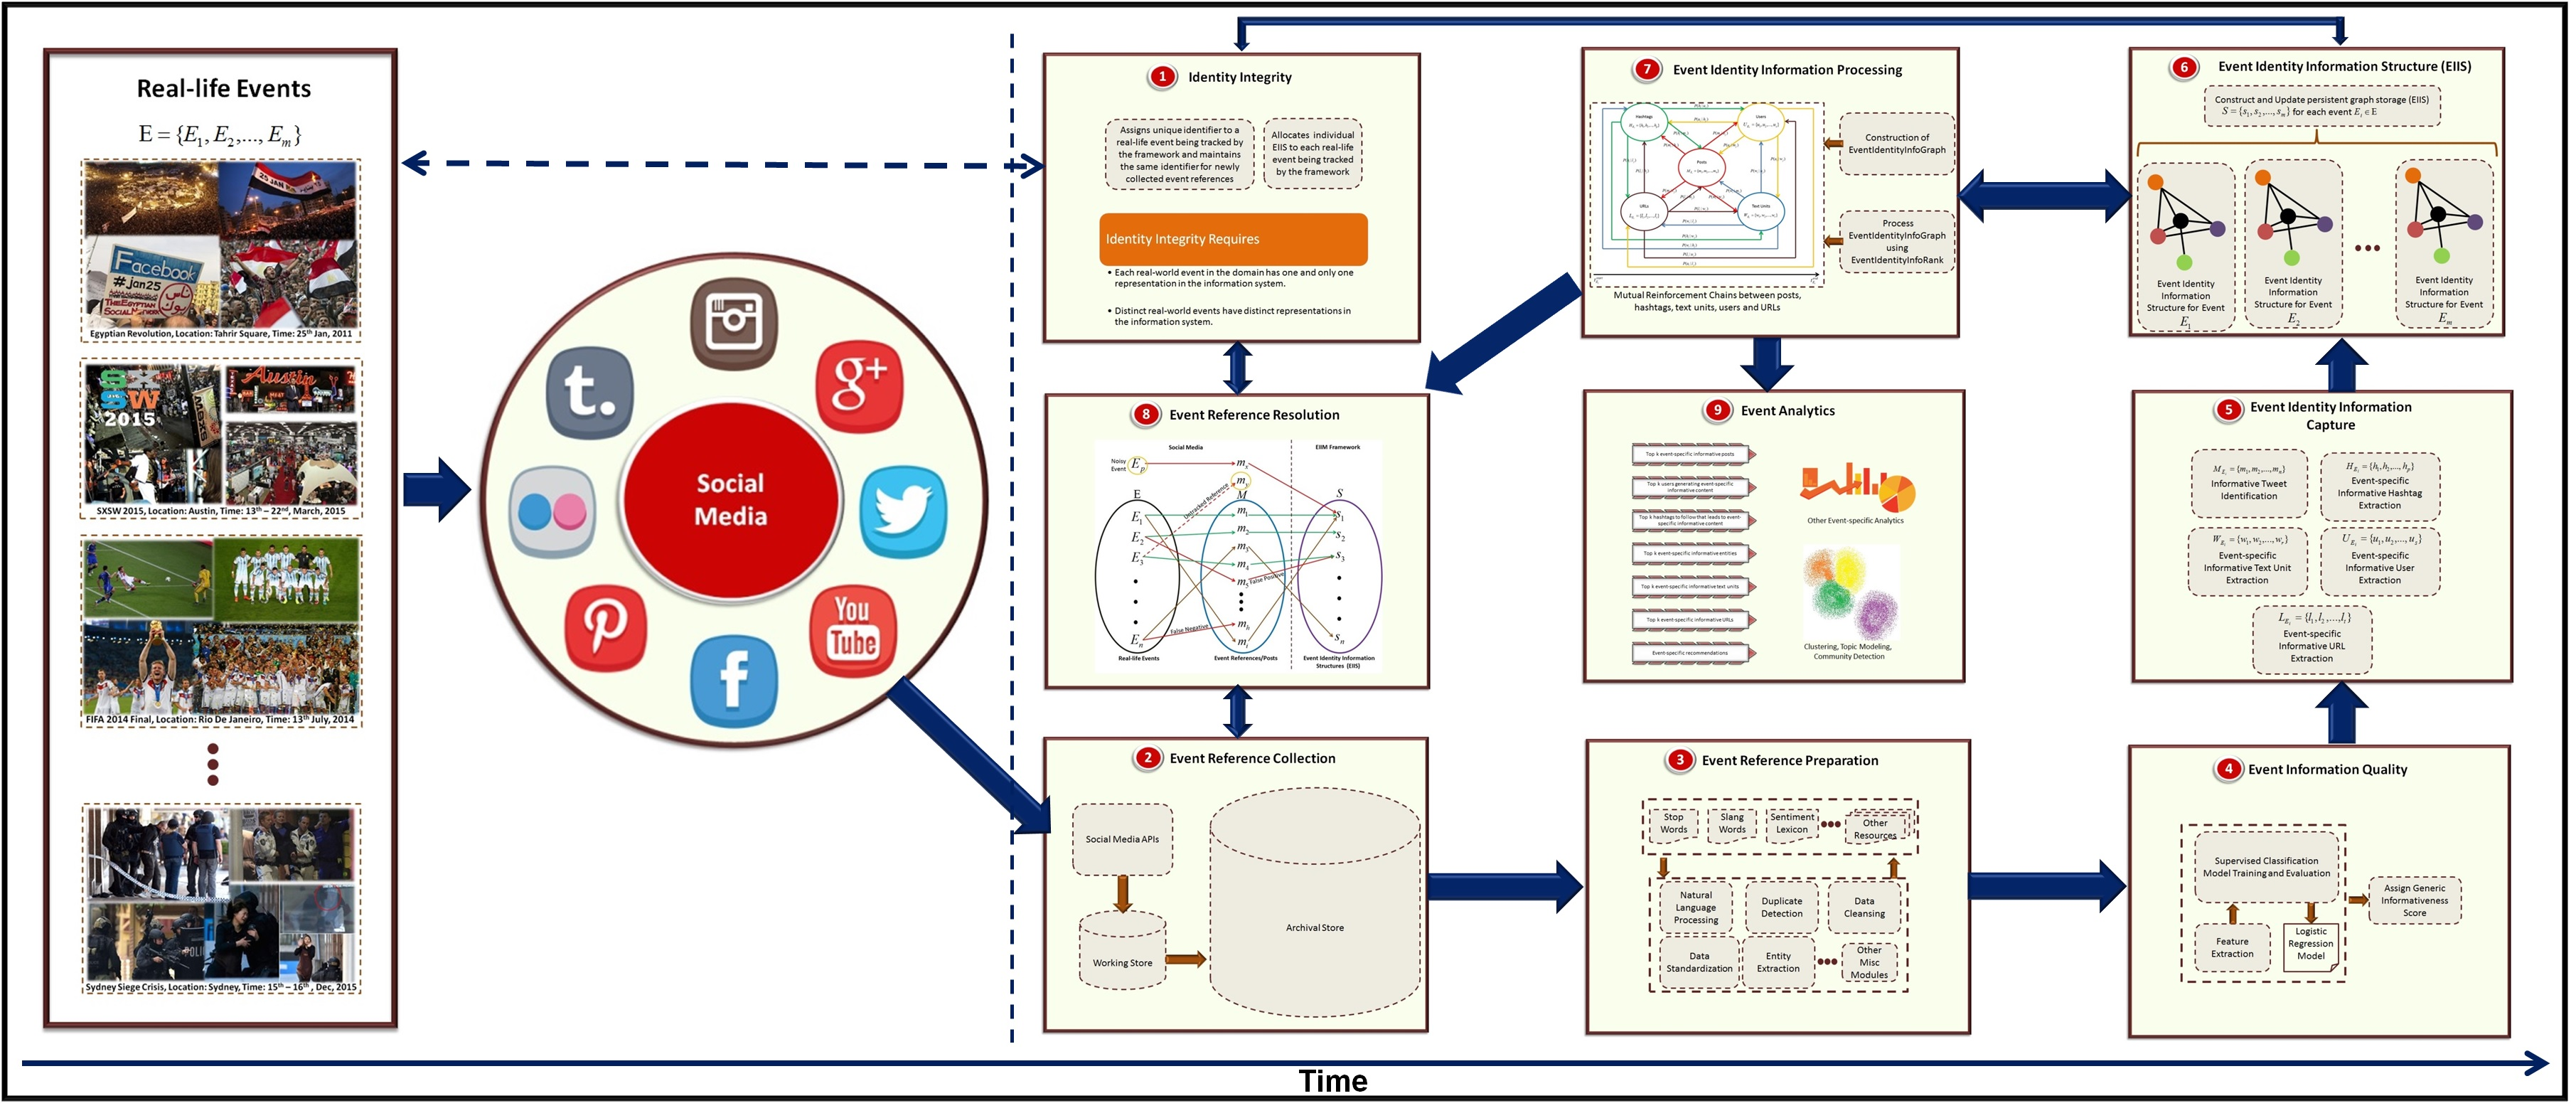
\includegraphics[width=15.5cm,height=7cm]{Figures/EIIM.jpg}
\end{figure}

Some of the main contributions of the work are:

\begin{itemize}
\item Extending the Entity Identity Information Management model  \cite{zhou2011entity} from the closed world domain of Master Data Management (MDM) to the open and unstructured domain of social media.

\item Design and implementation of an \textit{Event Identity Information Management} framework that is capable of tracking and identifying event-specific information from long as well as short user generated textual content in social media. Towards this objective a data processing pipeline named \textit{Event Identity Information Management Life Cycle} is developed (Figure \ref{eiim}), which is capable of :
\begin{itemize}
\item collecting event related real-time content generated in social media
\item pre-processing them using natural language processing techniques
\item identifying high quality informative sources of information
\item extracting event-specific information in order to create \textit{Event Identity Information Structures} (EIIS) for persistently storing and characterizing the salient and high quality event related information 
\item identifying event-specific informative content produced in social media
\end{itemize}


\item Implementation of a supervised classifier in the domain of short and informal social media textual content, for segregating high quality informative messages having higher chances of containing event related information from the low quality non-informative ones. 

\item Analysis of informative and non-informative event related content from 3.8 million short textual social media messages.

\item A novel model that leverages mutually reinforcing relationships between blog posts and named entities mentioned in them, and simultaneously ranks blogs as well as the named entities, allowing identification of event-specific content and further analysis of event-specific information.

\item A novel model based on principle of mutual reinforcement that takes into account the semantics of relationships between short textual \textit{social media messages}, \textit{hashtags}, \textit{text units}, \textit{URLs} and \textit{users}, and represent them in a graph structure - \textit{EvenIdentitytInfoGraph}. A scalable graph processing iterative algorithm -\textit{EventIdentityInfoRank}, is implemented for ranking the nodes of the \textit{EventIdentityInfoGraph}. The algorithm is capable of simultaneously ranking \textit{social media messages}, \textit{hashtags}, \textit{text units}, \textit{URLs} and \textit{users} in terms of event-specific informativeness providing deeper insights into the identity of an event.

\item Evaluate the proposed techniques against popularly used baseline techniques using large scale datasets.

\end{itemize}

Our research publications as well as upcoming publications that represents our contributions related to specific areas covered by the broad area of research as presented in this thesis are given below.

\textbf{\LARGE Related Filed Patent}
\begin{itemize}
\item A System for Collecting, Ranking and Managing Entity Identity Information from Social Media (US 62135258). Inventors: \textbf{Debanjan Mahata} and John R. Talburt, Assignee: The Board Of Trustees Of The University Of Arkansas.
\end{itemize}

\textbf{\LARGE Related Award}
\begin{itemize}
\item \textbf{Debanjan Mahata} and John R. Talburt. \textit{Chatter that Matter : A Framework for Collecting, Extracting, and Managing Event Identity Information from Short Social Media Text}. Student Research and Creative Works Expo, Graduate Competition, University of Arkansas at Little Rock, April, 2015. (Awarded First Place in Engineering and Information Technology).  
\end{itemize}

\textbf{\LARGE Related Publications}
\begin{itemize}
\item \textbf{Debanjan Mahata}, John R. Talburt and Vivek Kumar Singh; \textit{Identifying and Ranking of Event-specific Entity-centric Informative Content from Twitter}. $20^{th}$ International Conference On Applications Of Natural Language To Information Systems (NLDB 2015), Passau, Germany. $17^{th}-19^{th}$ June, 2015.

\item \textbf{Debanjan Mahata} and John R. Talburt; \textit{A Framework for Collecting and Managing Entity Identity Information from Social Media}. $19^{th}$ International Conference on Information Quality, Xi'An, China.

\item \textbf{Debanjan Mahata} and Nitin Agarwal; \textit{Identifying Event-specific Sources from Social Media}. Online Social Media Analysis and Visualization. Lecture Notes in Social Networks, Springer, Kawash, Jalal (Ed). January, 2015.

\item Nitin Agarwal, \textbf{Debanjan Mahata}, and Huan Liu. \textit{Time-and Event-Driven Modeling of Blogger Influence}. Encyclopedia of Social Network Analysis and Mining. Springer New York, 2014. 2154-2165.


\item \textbf{Debanjan Mahata} and Nitin Agarwal. \textit{Learning from the crowd: An Evolutionary Mutual Reinforcement Model for Analyzing Events}. Advances in Social Networks Analysis and Mining (ASONAM), 2013 IEEE/ACM International Conference on. IEEE, 2013.

\item Nitin Agarwal, and \textbf{Debanjan Mahata}. \textit{Grouping the Similar among the Disconnected Bloggers}. Social Media Mining and Social Network Analysis: Emerging Research (2013), 54.

\item \textbf{Debanjan Mahata}, and Nitin Agarwal. \textit{What does everybody know? identifying event-specific sources from social media}. IEEE Fourth International Conference on Computational Aspects of Social Networks (CASoN), 2012.

\item \textbf{Debanjan Mahata} and Nitin Agarwal. \textit{Analyzing Event-specific Socio-Technical Behaviors Through the Lens of Social Media}. The International Sunbelt Social Network Conference (Sunbelt XXXII) organized by the International Network for Social Network Analysis (INSNA), March 12-18, 2012, Redondo Beach, California.

\item Vivek Kumar Singh, \textbf{Debanjan Mahata}, and Rakesh Adhikari. \textit{Mining the blogosphere from a socio-political perspective}. IEEE International Conference on Computer Information Systems and Industrial Management Applications (CISIM), 2010.

\item Vivek Kumar Singh, Rakesh Adhikari, and \textbf{Debanjan Mahata}. \textit{A clustering and opinion mining approach to socio-political analysis of the blogosphere}. IEEE International Conference on Computational Intelligence and Computing Research (ICCIC), 2010.

\end{itemize}

\textbf{\LARGE Related Submitted Publications}

\begin{itemize}
\item \textbf{Debanjan Mahata}, John R. Talburt, Vivek Kumar Singh and Rajesh Piryani; \textit{Chatter that Matter: A Framework for Identifying and Ranking Event-specific Informative Tweets}. $18^{th}$ International Conference on Text, Speech and Dialogue, Plzen, Czech Republic (Notification Due: May 10, 2015)

\item \textbf{Debanjan Mahata}, John R. Talburt and Vivek Kumar Singh; \textit{A Framework for Collecting, Extracting and Managing Event Identity Information from Twitter}. $20^{th}$ International Conference on Information Quality, M.I.T, Boston (Notification Due: April 30, 2015)

\item \textbf{Debanjan Mahata}, John R. Talburt and Vivek Kumar Singh; \textit{From Chirps to Whistles : Discovering Event-specific Informative Content from Twitter}. Proceedings of the $7^{th}$ Annual ACM Web Science Conference. ACM, 2015, Oxford, England (Notification Due: April 30, 2015)

\end{itemize}
  





 

%Twitter alone has 284 million monthly users,  posting 500 million tweets per day produces a variety of content\footnote{\tiny http://about.twitter.com/company}. A significant proportion of it are related to different real-life events (e.g, football matches, conferences, music shows, etc). Majority of this content are personal updates (e.g.  \textit{Thanks for the memories Sochi! I've had the time of my life \#Sochi2014 \#sochiselfie http://t.co/DqkLEaAMpo}), pointless babbles (e.g. \textit{Ted Cruz is a dangerous man. Crazy and gaining support. Megalomaniac leaders are bad, mkay. \#CPAC \#politics \#joke}) and spams (e.g \textit{New post: Sochi Was For Suckers - Laugh Studios/ http://t.co/cWQJCBp3Ow \#lol \#funny \#rofl \#funnypic \#wtf.}). Personal views and conversations might be of interest to a specific group of people. However, they are meaningless and provides no information to the general audience. On the other hand there are tweets that presents newsworthy content, recent updates and real-time coverage of on-going events (e.g. \textit{In \#Sochi, the Dutch are dominating the overall Olympic medal count http://t.co/jMR1WUqEK4 (Reuters) http://t.co/dAfDhEgTGA}). These tweets provide event-specific informative content and are more useful for general audience interested to know about the event. We call them as event-specific informative references. Table \ref{tweetsample} presents some examples of different types of tweets shared during real-life events.
%
%\begin{table}[htbp]
%\centering
%\caption{Examples of different event related tweets.}
%\label{tweetsample}
%     \begin{tabular}{|p{14cm}|} \hline
%     Ted Cruz is a dangerous man. Crazy and gaining support. Megalomaniac leaders are bad, mkay. \#CPAC \#politics \#joke [\textit{\textbf{personal/uninformative}}] \small \textit{\textbf{Event: `CPAC 2014'}}\\ \hline
%     Thanks for the memories Sochi! I've had the time of my life \#Sochi2014 \#sochiselfie http://t.co/DqkLEaAMpo. [\textit{\textbf{personal/uninformative}}] \small \textit{\textbf{Event: `Sochi Games'}} \\ \hline
%     \#SXSW14 \#SXSW \#sxswinteractive \#CPAC2014 \#CPAC \#CPACPickupLines \#CPACPanels Be squared away \@ perky TOP TWEETED of http://t.co/h0igdOVNW0. [\textit{\textbf{spam/uninformative}}] \small \textit{\textbf{Event: `CPAC 2014'}}\\ \hline
%In \#Sochi, the Dutch are dominating the overall Olympic medal count http://t.co/jMR1WUqEK4 (Reuters) http://t.co/dAfDhEgTGA. [\textit{\textbf{event-specific informative}}] \small \textit{\textbf{Event: `Sochi Games'}}\\ \hline
%New post: Sochi Was For Suckers - Laugh Studios/ http://t.co/cWQJCBp3Ow \#lol \#funny \#rofl \#funnypic \#fail \#wtf. [\textit{\textbf{spam/uninformative}}] \small \textit{\textbf{Event: `Sochi Games'}}\\ \hline
%It's \@tedcruz vs. \@SenJohnMcCain in a \#CPAC spat. What did they say? Find out on \#AC360 8p on \@CNN. [\textit{\textbf{event-specific informative}}] \small \textit{\textbf{Event: `CPAC 2014'}} \\ \hline
%     \end{tabular}
%\end{table}


%\section{Background : Entity Identity Information Management in Master Data Management}
%
%
%
%\section{Problem Definition and Research Questions}
%
%\section{General Challenges in Mining Social Media Text}
%
%\subsection{Information Overload}
%A daily average of 58 million tweets is posted in Twitter\footnote{http://www.statisticbrain.com/twitter-statistics/}.On an average 60 million  photos are shared in Instagram daily\footnote{http://instagram.com/press/}. Facebook stores 300 petabytes  of data related to its users from all over the world\footnote{http://expandedramblings.com/index.php/by-the-numbers-17-amazing-facebook-stats/}. These are some compelling statistics that makes social media not only rich in volume of data, but also variety, and the velocity at which data is being generated. Due to the great pace at which data is produced in social media, the search engines and content filtering algorithms often face the problem of information overload \cite{hemp2009death}. They suffer from the dilemma of assessing the accuracy and quality of information content in the sources being produced over their freshness. Thus, collecting different types of references of entities from various social media platforms, assessing their quality, resolving and extracting identity information of the entities poses great challenges in such a situation.
%
%\subsection{Veracity of Sources}
%Judging the accuracy of the information and deciding relevant information content in social media references for the purpose of extracting entity identity attributes constitutes another challenging situation. For trending topics the search engines have started showing real-time feeds from social media websites in their search results. This has attracted spammers who post trending hash-tags or keywords along with their spam content in order to attract people to their websites offering products or services \cite{benevenuto2010detecting}. An alarming 355\% growth of social spam has been reported in 2013\footnote{http://www.likeable.com/blog/2013/11/10-surprising-social-media-statistics/}. Social media has also been instrumental in spreading misinformation and rumors. Spread of misinformation not only results in pandemonium among the users\footnote{http://www.theguardian.com/uk/interactive/2011/dec/07/london-riots-twitter}  but also result in extraction of completely wrong information about entities.
%
%\subsection{Informal Text}
%Unlike sources of news media and edited documents on the web, the textual content of the social media sources are highly colloquial and pose great difficulties in extracting information. One of the most important sources of information about events, prevalent in the domain of social media are the micro-blogging platforms. Micro blogs pose additional challenges due to their brevity, noisiness, idiosyncratic language, unusual structure and ambiguous representation of discourse \cite{bontcheva2013twitie}. Variation in language, less grammatical structure of sentences, unconventional uses of capitalization, frequent use of emoticons, and abbreviations have to be dealt by any system processing social media content. Moreover, various signals of communications embedded in the text in the form of hash-tags (eg.\#sochi), retweets (RT) and user mentions (@) should be understood by the system in order to extract the contextual information hidden in the text. Intentional misspellings sometimes demonstrate examples of intonation in written text \cite{prevost1996information}. For instance, expressions like, `this is so cooool', emphasizes stress on the emotions and conveys more information that should be captured. It has been shown that it is extremely challenging for the state-of-the art information extraction algorithms to perform efficiently and give accurate results for micro-blogs \cite{derczynski2013microblog}. For example, named entity recognition methods typically show 85-90\% accuracy on longer texts, but 30-50\% on tweets \cite{ritter2011named}. Status messages in social networking websites, content in question answering websites, reviews, and discussions in blogs, and forums exhibit similar nature and present similar challenges to information extraction and text mining procedures.
%
%
%
%\subsection{Sampling Bias}
%Most commonly used method for obtaining data samples from social media websites is by using their application programming interfaces (APIs). Given the humungous amounts of data produced in real-time, the APIs cannot provide all the data to every single API requests. The requests are often made through a query interface by passing certain query parameters to the APIs. The amount of data returned against the queries may vary. This depends upon the popularity of the content related to the query. For example, in Twitter studies have estimated that by using Twitter's Streaming API users can expect to receive anywhere from 1\% of the tweets to over 40\% of tweets in near real-time\footnote{https://www.brightplanet.com/2013/06/twitter-firehose-vs-twitter-api-whats-the-difference-and-why-should-you-care/}. The only way to get access to all the tweets is to buy the firehose service, which is seldom done for academic purposes. Other real-time social media publishing services mostly follow the same model. Therefore, this might lead to biasness in the samples collected for studying event related phenomenon and for tracking all the important event related information being produced in real-time.
%
%\subsection{Multiple Data Sources}
%The APIs (Application Programming Interfaces) of the different social media websites returns data in different formats (JSON, XML) using different web standards (REST, HTTPS). Moreover, the information obtained from a social media website is dependent upon the type of content it produces. A video sharing website might return an entirely different set of information from a blogging website. Thus, integrating the data obtained from the various social media platforms for the purpose of extraction and tracking of event related information is also one of the challenges.
%
%\subsection{Lack of Evaluation Datasets}
%There is a lack of ground truth evaluation data for most of the social media text mining tasks. In traditional data mining research, there is often two types of datasets. One of them is known as training dataset and the other is known as test dataset. The models are trained or developed using the training datasets and are evaluated on test datasets. Thus, the test datasets act as the ground truth. The test dataset for various text mining tasks is mostly not available for social media data. It is often the duty of the researchers to create new test datasets in order to solve a specific task in social media. Sometimes this data might not be a benchmark dataset due to various unwanted noise and human error or perception in annotating the data. This might lead to wrong assumptions and false results.
%
%
%\section{Research Methodology}
%
%\section{Research Contributions}
%

The rest of the thesis is organized as follows:

Chapter \ref{events} gives an overview of the different social media websites and challenges in mining information from them. It also looks at the different perspectives of defining an event and gives the definition of events in social media as accepted by the presented work. Finally, it defines the problem of Event Identity Information Management from Social Media whose solution and application is extensively discussed throughout the rest of the thesis.

Chapter \ref{review} reviews the existing literature related to the topic of the thesis and highlights the challenges in applying previously available techniques to the domain of social media. It also discusses the similarities and dissimilarities of our work with the previous ones, and identifies the areas of our novel contributions that makes it different from the available techniques.

Chapter \ref{eiim} presents a detailed discussion of the \textit{Event Identity Information Management Life Cycle}, that is proposed as a solution to the problem that is solved in this thesis. It goes through all the components of the life cycle and gives a detailed explanation of the design choices, implementation and their working.

Chapter \ref{applications} highlights the potential real-life application of the \textit{Event Identity Information Management} framework implemented in this thesis. 

Chapter \ref{Conclusion} draws conclusions of the work presented in this thesis and points to future directions of the work.

%% Chapter 2

\chapter{Defining Events} % Main chapter title

\label{EventDefinition} % For referencing the chapter elsewhere, use \ref{Chapter1} 

\lhead{Chapter 2. \emph{Defining Events}} % This is for the header on each page - perhaps a shortened title

\section{Topic Detection and Tracking}

\section{Automatic Content Extraction}

\section{Multimedia Event Detection}

\section{Events in Social Media} 
%% Chapter 3

\chapter{Defining Events} % Main chapter title

\label{EventDefinition} % For referencing the chapter elsewhere, use \ref{Chapter1} 

\lhead{Chapter 3. \emph{Defining Events}} % This is for the header on each page - perhaps a shortened title

\section{Topic Detection and Tracking}

\section{Automatic Content Extraction}

\section{Multimedia Event Detection}

\section{Events in Social Media}
%% Chapter 4

\chapter{Identifying Event-specific Sources from the Blogosphere} % Main chapter title

\label{BlogStudy} % For referencing the chapter elsewhere, use \ref{Chapter1} 

\lhead{Chapter 4. \emph{Identifying Event-specific Sources from the Blogosphere}} % This is for the header on each page - perhaps a shortened title

\begin{abstract}
 Social media has become a useful medium for mobilizing support for various real-life events and a platform for the public to voice their opinion freely to a huge audience in the web. Social media sources often provide novel and specific information in contrast to the generic information obtained from the mainstream media. This makes social media a valuable source for conducting studies and analyzing events. However, due to the power law distribution of the Internet, these sources get buried in the Long Tail. The overwhelming number of Long Tail social media sources makes it more challenging to identify the valuable sources with specific information. It is, therefore, of utmost importance to identify quality sources from these social media sites for understanding and exploring an event. We propose an evolutionary mutual reinforcement model for identifying and ranking highly `specific' social media sources, otherwise buried in the Long Tail, and `close' entities related to an event. We also introduce a novel evaluation strategy, due to the absence of ground truth for validating the results. We observe a huge percentage gain in information between 25\% and 130\% against the baselines (viz., Google search and Icerocket blog search) from the sources ranked according to our model. Further, our ranking methodology is capable of identifying the highly informative sources much earlier than the widely-used baselines. Our model also shows its potential as an apparatus to analyze events at micro and macro scales. Data for the research is collected from various blogging platforms like blogspot, livejournal, wordpress, typepad, etc. and will be made publicly available for researchers.
\keywords{event analysis, social media, mutual reinforcement, specificity, closeness, information gain}
\end{abstract}


\section{Introduction}

Social media has brought a paradigm shift in the way people share information and communicate.  Social media played an important role in mobilizing events such as, `The Arab Spring', `Occupy Wall Street', `Sandy relief efforts', `London Riots',`The Spanish Revolution', among others. This led to a surge in citizen journalism all over the world, encouraging transnational participation. Thus, social media serves as a parallel, yet distinct source of information about real-life events along with the mainstream media space \cite{reese2007mapping}.

The mainstream media sources often gloss over the intricate details while covering a real-life event. They are often biased, regulated by the government, and may not portray the true picture of an event \cite{hamdy2012framing}. While, social media sources like blogs often contain unbiased, uninhibited, and unedited opinions from people. Blogs have been accepted as more credible sources of information over mainstream media sources by the weblog users \cite{johnson2004wag}. Thus the sources, which are obtained from social media could potentially provide a rather `closer'  or an ``on-ground" view of the events with novel information. The ``on-ground'" information gleaned from the social media affords opportunities to study various online social phenomenon from methodological and theoretical perspectives including, social movements, crowdsourcing, citizen journalism, collective behavior, collective action \cite{agarwal2011finding,agarwal2012online,agarwal2012raising}, and more.

\begin{figure}[htb]
\centering
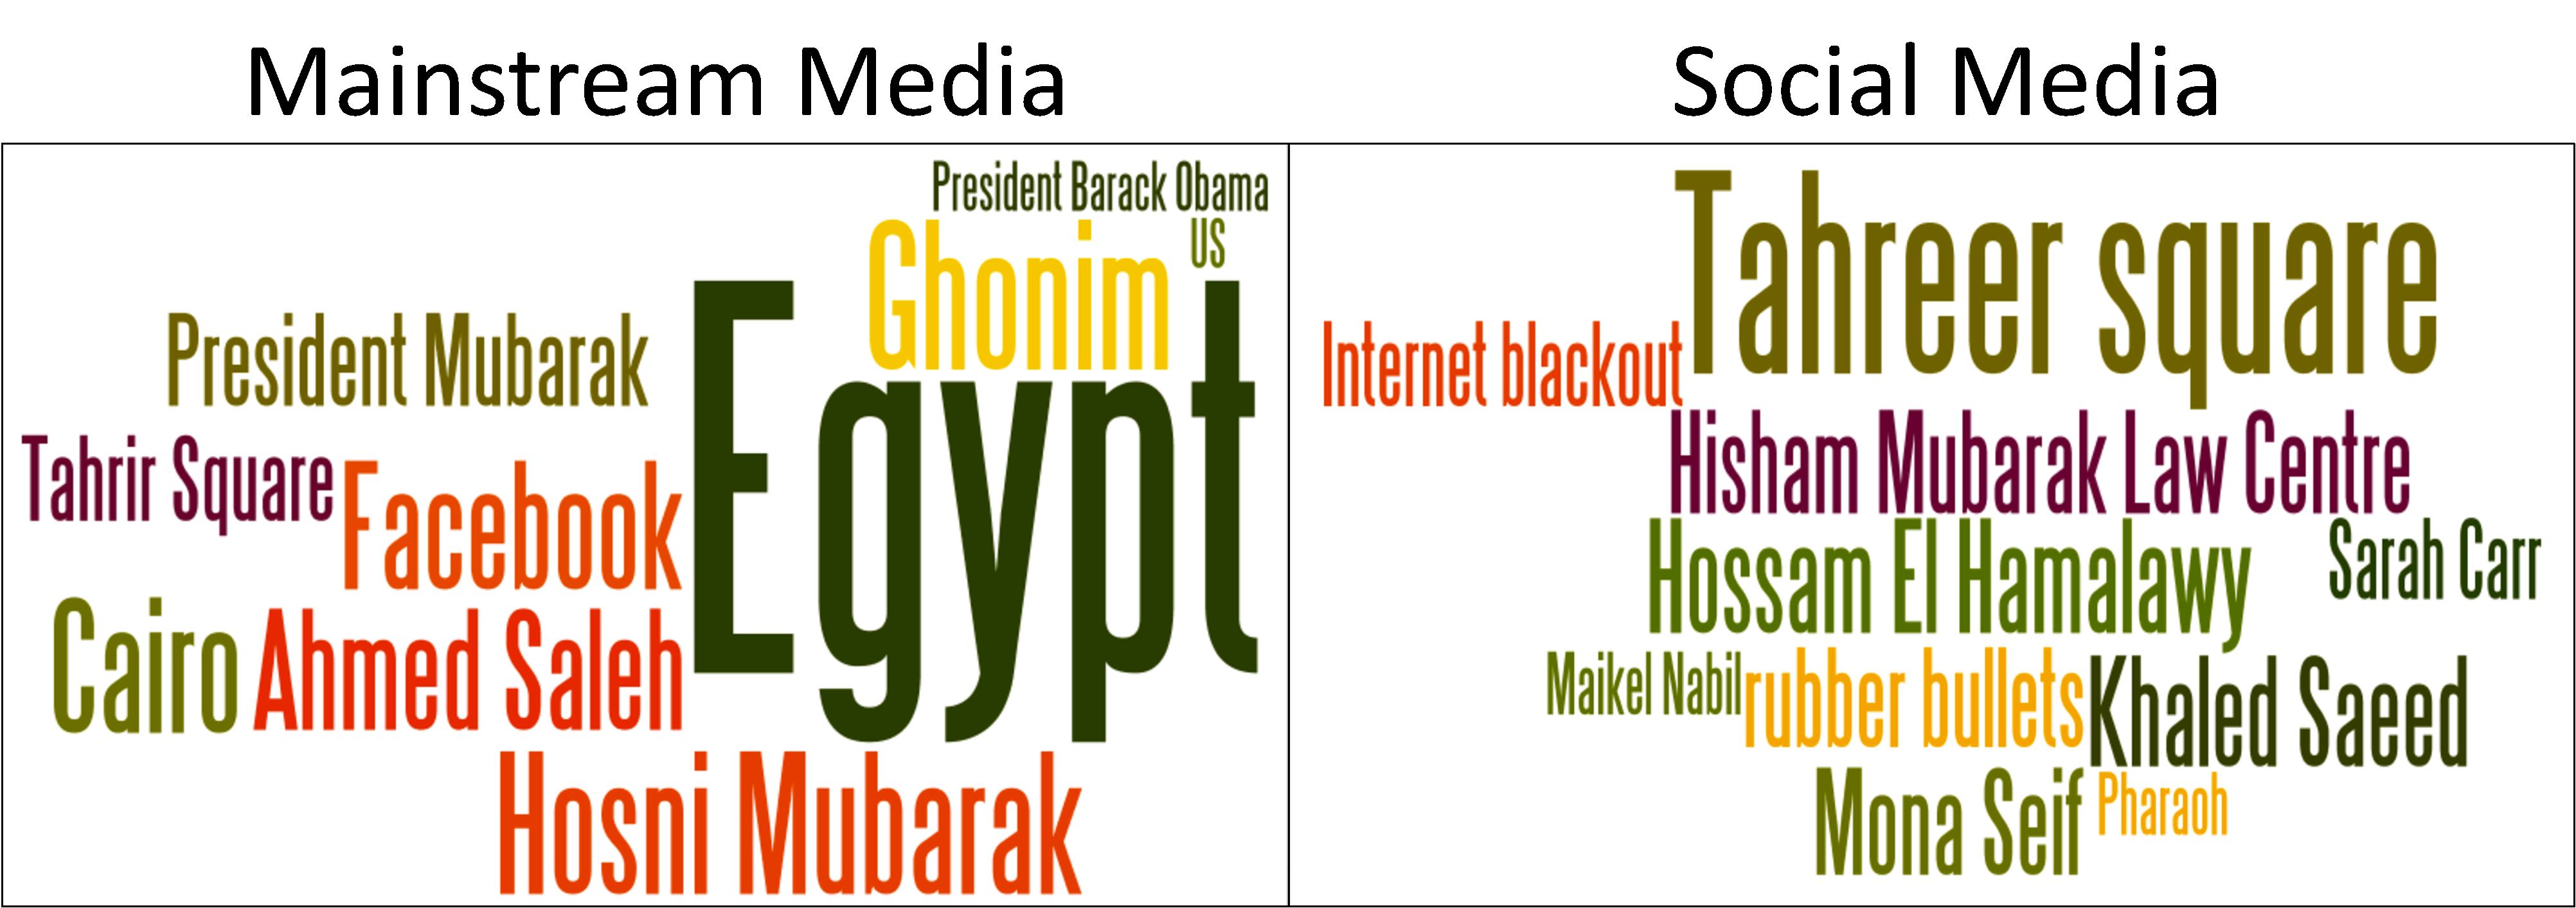
\includegraphics[height=2in,width=4.5in]{Figures/Chapter3Figures/comp.pdf}
\caption{Top 10 entities from mainstream media and blogs.}
\label{fg:comp}
\end{figure}

\noindent \textbf{\textit{Motivation:}} An initial analysis of the top 10 entities obtained from the top 10 search results related to ``Egyptian Revolution'' from two mainstream media channels (BBC and CNN), and from blogs during the time of the revolution is shown in Fig~\ref{fg:comp}. The top entities from the mainstream media channels are generic and are quiet obvious for the event. In contrast, the top entities from the blogs are very specific to the event. The activists like `Mona Seif', `Sarah Carr', `Maikel Nabil' and `Hosam El Hamalwy' were very closely involved, and were responsible for mobilizing the event. The entities like `Internet Blackout' and `Khaleed Saeed' were central to the event. Moreover, the presence of entities like `Facebook' and `Ghonim' (who was responsible for spreading the event in Facebook) among the top mainstream media entities also indicates the significance of social media in the event.

\begin{figure}[htb]
\centering
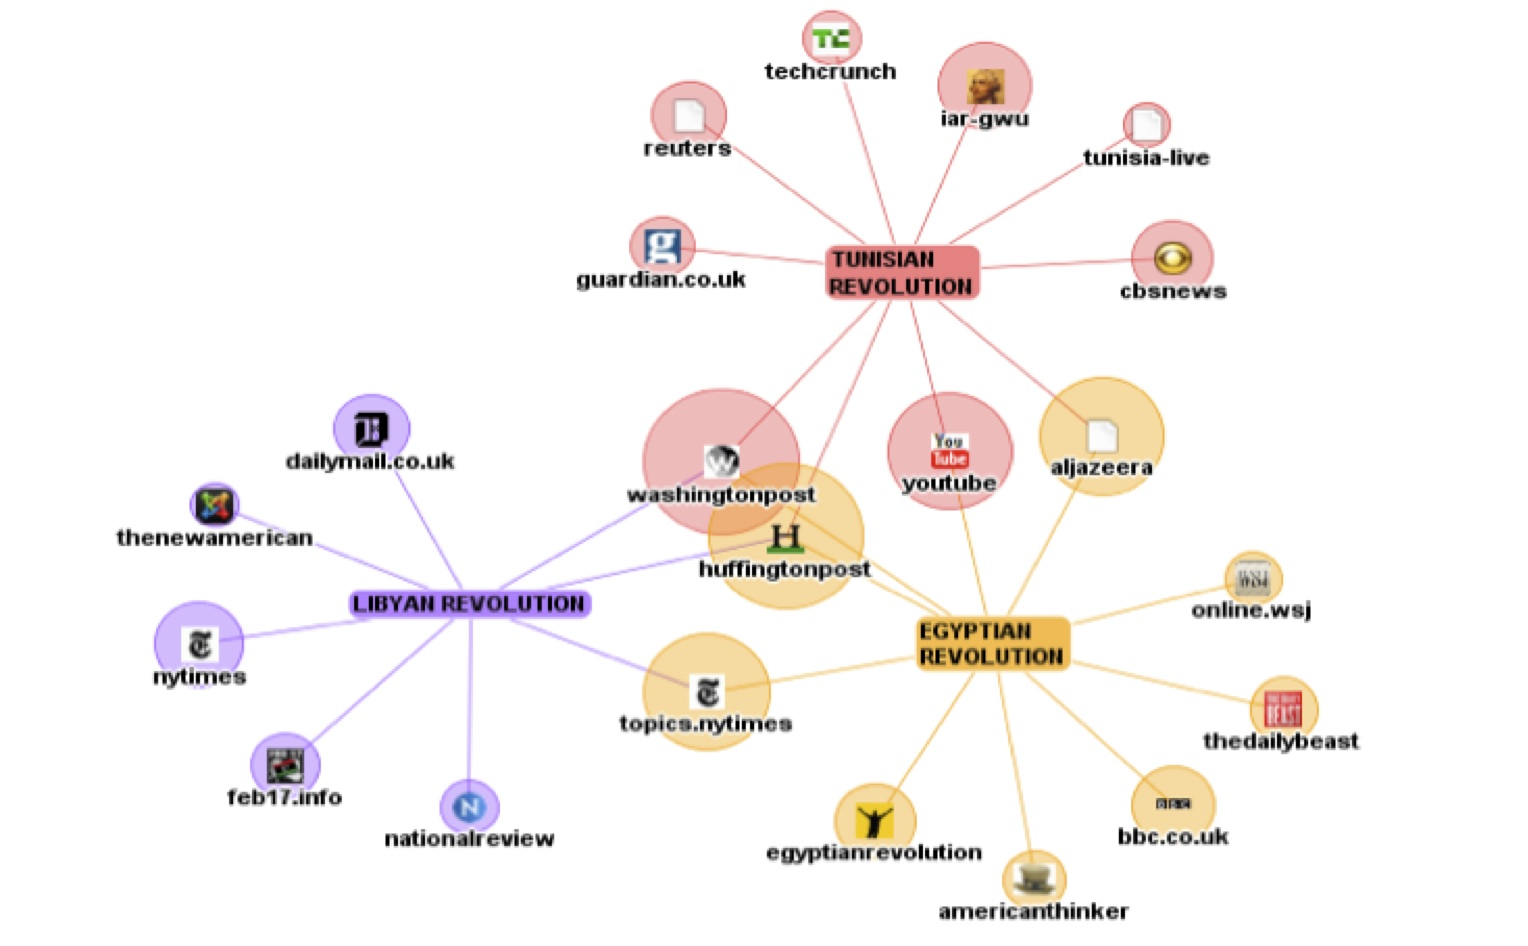
\includegraphics[height=3.5in,width=4.5in]{Figures/Chapter3Figures/touchgraph.jpg} 

\caption{\small Top 10 Google search results for ``Egyptian Revolution'', ``Libyan Revolution'', and ``Tunisian Revolution'', visualized using TouchGraph.}

\label{fg:touchgraph}

\end{figure}

Due to the power law distribution of the Internet \cite{adamic2000power}, and the present search engine technology, the `Short Head' is generally dominated by the mainstream media websites. As illustrated in Fig ~\ref{fg:touchgraph} the top 10 search results for ``Egyptian Revolution", ``Libyan Revolution", and ``Tunisian Revolution" by Google, visualized using Touchgraph\footnote{http://touchgraph.com}, retrieved mainstream media sources. Consequently, the social media sites get buried in the Long Tail \cite{LOmariba} as shown in Fig ~\ref{fg:longvsshort}. However sources from the social media channels, act as hubs of specific information about real-life events \cite{harb2011arab}. Thus, a person interested to analyze an event may miss out the novel and specific information available in social media by relying on the top results from the popular search engines. Moreover, in the words of Chris Anderson \cite{anderson2008long}, \begin{itshape} \small ``With an estimated 15 million bloggers out there, the odds that a few will have something important and insightful to say are good and getting better.'' \end{itshape} This motivated us to look for techniques in this paper, that would help in identifying these otherwise buried sources providing highly specific information related to an event.

\paragraph
\noindent \textbf{\textit{Challenges:}} Identifying highly informative `specific' sources and `close' entities related to a real-life event from social media entails various challenges as follows,
\begin{itemize}
\item \textbf{Sparsity of sources:} Enormous population of the sparsely linked Long Tail social media sources %\cite{agarwal2008identifying}% makes it challenging to identify and collect quality sources. 


\item \textbf{Quality assessment dilemma:} The entities (person, organization, place, etc.) mentioned in the sources act as the atomic units of information. Sources which are `specific' to an event must contain entities `closer' or highly relevant to the event. On the other hand, such `close' entities can be obtained from the `specific' sources. This presents a dilemma in assessing the quality of the sources for event related `specific' information content, and makes it a nontrivial task. 

\item \textbf{Entity extraction:} It is also a challenge, to accurately extract the entities from the social media sources, which are mostly unstructured and have colloquial content. 

\item \textbf{Lack of evaluation measures:} Conventional information retrieval based evaluation measures help in identifying the most relevant and authoritative sources, however, these sources may not be the most novel or offer specific information. Therefore, new evaluation measures are required to estimate the performance of our work.

\end{itemize}


\begin{figure}[htb]
\centering
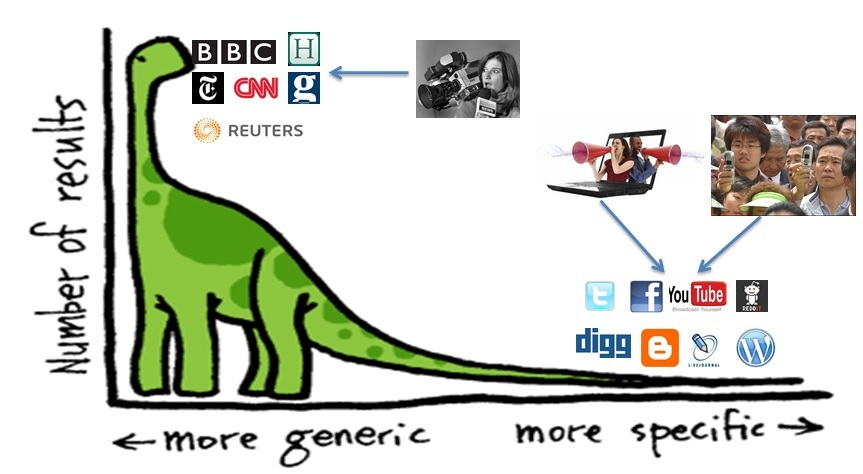
\includegraphics[height=3.3in,width=4.8in]{Figures/Chapter3Figures/LongTailVsShortHead.jpg} 

\caption{\small Short Head Vs Long Tail media sources.}

\label{fg:longvsshort}

\end{figure}

\paragraph
\noindent \textbf{\textit{Contributions:}} We make the following contributions,
\begin{itemize}
\item \textbf{Methodology:} A methodology based on the principle of mutual reinforcement, that helps in identifying highly `specific' sources and `close' entities from social media, and their relationships (Section \ref{mutual}). It ranks the sources and the entities based on their `specific' information content and how `close' they are with respect to a set of events.

\item \textbf{Evaluation Strategy:} Present the methodology, along with an objective evaluation strategy to validate our findings (Section \ref{basecomp}). 

\item \textbf{Experiment on sources related to real-life events:} Perform our experiments on sources and entities related to the events: `Egyptian Revolution', `Libyan Revolution', and `Tunisian Revolution' (Section \ref{exp}). However, the work is extendible to other types of events. 

\item \textbf{Event analysis:} Explore the utility of such a model in analyzing events (Section \ref{explore}) and conclude the work with future directions (Section \ref{future}).
\end{itemize}

Next, we present the related work and compare and contrast  these with the proposed approach, highlighting our contributions to the literature.

\section{\label{sec:related}\textbf{Related Work}}
In this section, we discuss about some of the previous research relevant to our work. We present studies on analyzing real-life events, identifying quality sources related to them and in general from the web.

User-generated data from various social media platforms, related to real-life events, have been studied to perform wide range of analysis. Socio-political inferences were drawn by studying sentiments and opinions of people towards public and political events from Twitter \cite{younus2011average}, as well as blogs \cite{singh2010mining}. Twitter has been extensively used as a source for analyzing information circulated during natural disasters and crisis situations \cite{vieweg2010microblogging,cheong2011social}. Tweets related to events have been extracted, summarized and visualized, in order to have a deeper understanding of the events \cite{marcus2011twitinfo,popescu2011extracting}. 

Our work is different from all such works, and would help in analyzing events from sources and entities, which are highly specific to an event along with the generic ones.

Due to huge number of informal sources in social media it is a difficult task to identify high quality sources related to the real-life events. Researchers have built semantic web models for efficient retrieval of event specific media sources \cite{troncy2010linking}. Event related contents have been found leveraging the tagging and location information associated with the photos shared in Flickr \cite{rattenbury2007towards}. \textit{Becker et al} \cite{becker2011selecting}, studied how to identify events and high quality sources related to them from Twitter. In order to identify the genuine sources of information, credibility and trustworthiness of event related information were studied from Twitter \cite{gupta2012evaluating}. New methods were investigated for filtering and assessing the verity of sources obtained from social media by journalists \cite{diakopoulos2012finding}. 

The work presented in this paper, finds quality sources related to an event from social media, in terms of the `specific' information content of the source, and is quiet different from all such works.

Several methods have been developed in the past for identifying and ranking quality sources from the web. PageRank \cite{brin1998anatomy} took advantage of the link structure of the web for ranking web pages. It was further improved for making it sensitive to topic based search \cite{haveliwala2003topic}. Graph based approaches were used for modeling documents and a set of documents as weighted text graphs, and for computing relative importance of textual units for Natural Language Processing \cite{erkan2004lexrank}. Mutual reinforcement principle was used for identifying Hubs and Authorities from a subset of web pages \cite{kleinberg1999authoritative}. 

Our work is distinct from all such works. The methodology of our work utilizes the relationship between sources and entities related to a real-life event. It then builds upon the principle of mutual reinforcement and modifies it to a evolutionary system for finding `specific' sources and `close' entities w.r.t an event (Subection \ref{mutual}). A comparative analysis with the conventional mutual reinforcement demonstrates a faster convergence and better performance of our evolutionary model (Subsection \ref{compconvevol}). Our framework also has the potential to be used as an apparatus for studying events in terms of the specific sources and close entities identified and ranked by our proposed methodology (Section \ref{explore}). Next, we present the formal problem definition.




\section{\label{problemdef}\textbf{Problem Definition}}

The number of sources related to an event in social media is overwhelming. All these sources may not provide useful information and needs to be processed in order to identify the valuable
sources providing specific information about the concerned event. Provided we have a set of events, a set of sources, and a set of entities related to each of these events, we need to rank these sources and entities from the most specific to the most generic ones, based on their information content.

\begin{figure}[htbp]
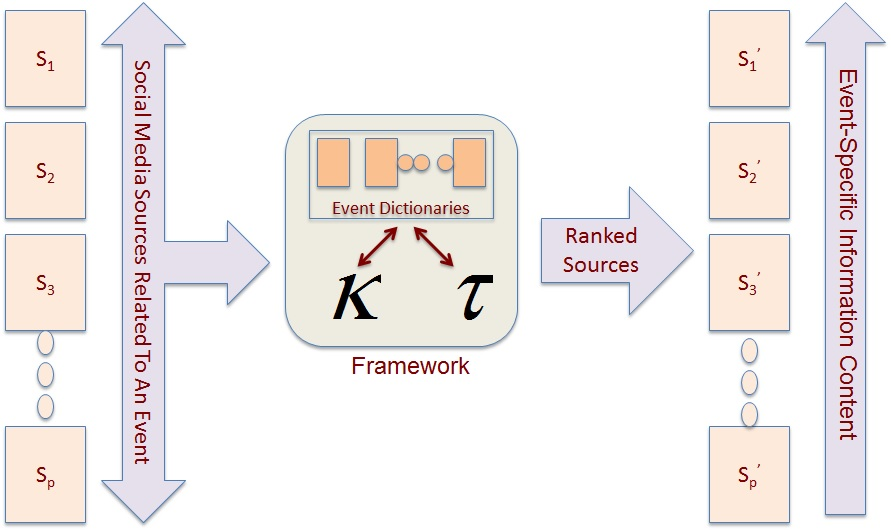
\includegraphics[height=3in,width=4.8in]{Figures/Chapter3Figures/frameworkIllustrated.jpg} 
\caption{\small Black box view of the problem.} 
\label{fg:problem}
\end{figure}

\paragraph
\noindent \textbf{Event:} \begin{itshape}We define an event to be a real-world incident, occurring at any place at any time or over a certain period of time.\end{itshape}

\paragraph
\noindent \textbf{Specificity and Closeness:} \begin{itshape}
\noindent Given a finite set of events $\xi$, we take an event $E_{j} \in \xi$ such that,  $1 \le j \le \mid \xi \mid$ , a set of `p' sources denoted by $\phi_{E_{j}}$, and a set of `q' entities denoted by $\sigma_{E_{j}}$, related to the event $E_{j}$. We define two functions $\kappa$ (\textit{specificity}) and $\tau$ (\textit{closeness}) such that:

\begin{equation}
\label{func1}
\kappa : S_{i} \rightarrow [0,1]
 \end{equation}

\begin{equation}
\label{func2}
\tau : e_{i} \rightarrow [0,1]
\end{equation}

\noindent where, $S_{i} (\in \phi_{E_{j}}$), is the $i^{th}$ source, and $e_{i} (\in \sigma_{E_{j}}$) is the $i^{th}$ entity, so that we can get two ordered sets ($\varphi_{E_{j}}$ and $\varsigma_{E_{j}}$) for the set of sources in $\phi_{E_{j}}$ and entities in $\sigma_{E_{j}}$, such that:

\begin{equation}
\varphi_{E_{j}} = \{S_{1},...,S_{i},S_{j},...,S_{p} \mid \kappa(S_{i}) \ge \kappa(S_{j}), i < j\}
\end{equation}

\begin{equation}
\varsigma_{E_{j}} = \{e_{1},...,e_{i},e_{j},...,e_{q} \mid \tau(e_{i}) \ge \tau(e_{j}), i < j\}
\end{equation}
\end{itshape}

\noindent $\varphi_{E_{j}}$ is ordered in decreasing order of how `specific' $S_{i}$ is w.r.t $E_{j}$. $\varsigma_{E_{j}}$ is ordered in decreasing order of how `close' $e_{i}$ is w.r.t $E_{j}$. 
A black-box view of the problem is shown in Fig ~\ref{fg:problem}.

\section{\label{method}\textbf{Methodology}}

\begin{figure*}[htb]
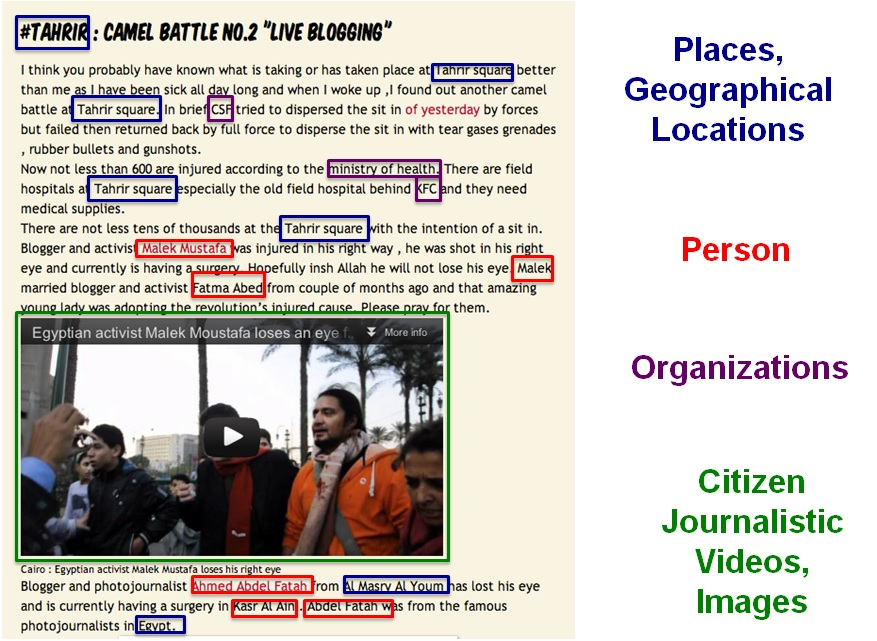
\includegraphics[height=3.8in,width=4.8in]{Figures/Chapter3Figures/entitySources.jpg} 
\caption{\small Entities associated with a social media source.} 
\label{fg:sourceEntities}
\end{figure*}


A real-life event is characterized by a distinct set of close entities (persons, places, organizations, etc.) along with generic ones. The entities act as the basic units of information in these sources as shown in Fig ~\ref{fg:sourceEntities}. Intuitively, specific sources would contain closer entities and one is likely to find closer entities in more specific sources. The relation between specific sources and close entities could then be modeled following the Mutual Reinforcement Principle, which forms the basis of our methodology.

%%%%%%%%%%%%%%%%%%%%%%%%%%%%%%%%%%%%%%%%%%%%%%%%%%%%%%%%%%%%%%%%%%%%
%\begin{quote}
%An entity $e_{i}$ should have high `closeness' score $(\tau(e_{i})_{E_{j}})$  w.r.t an event $E_{j}$ if it appears in many sources $(\in \varphi_{E_{j}})$ with high 'specificity' scores $(\kappa(S_{i})_{E_{j}}$ while a source should have a high 'specificity' score if it contains many entities with high 'closeness' scores.
%\end{quote}
%%%%%%%%%%%%%%%%%%%%%%%%%%%%%%%%%%%%%%%%%%%%%%%%%%%%%%%%%%%%%%%%%%%%

\begin{quote}
An entity should have high `closeness' score if it appears in many sources with high 'specificity' scores while a source should have a high 'specificity' score if it contains many entities with high 'closeness' scores.
\end{quote}

In essence the principle states that the 'closeness' score of an entity is determined by the 'specificity' scores of the sources it appears in, and the 'specificity' score of a source is determined by the 'closeness' scores of the entities it contain. The proposed methodology extends the basic Mutual Reinforcement Principle to consider the evolving knowledge learned about an event. However, the model requires an apriori or seed knowledge about an event, which is provided in terms of an event profile or an event dictionary. Next, we discuss the construction of event dictionaries.

\subsection{\label{eventdict}\textbf{Event Dictionaries}}
Each event $E_{j}$ is profiled by constructing an event dictionary ($\sigma_{E_{j}}$). In order to calculate specificity of a source w.r.t an event, we need to start with an initial set of close entities. At the same time, these close entities are better acquired from the specific sources. To solve this dilemma, we construct event dictionaries, from independent sources which are completely separate from the sources ($\phi_{E_{j}}$) that need to be ranked. 

\paragraph
\noindent \textbf{\textit{Formulation of initial closeness scores:}} We calculate the `closeness' score ($\tau(e_{i})_{E_{j}}$) of each entity ($e_{i}$) for event $E_{j}$  in order to construct the event dictionaries, by using equations \ref{tfidf1} and \ref{tfidf2} based on tf-idf  measure \cite{ramos2003using} , from the information retrieval literature. Let $E_{j} \in \xi$, be the $j^{th}$ event, and `$e_{i}$' be the $i^{th}$ entity extracted from the set of sources selected for constructing the event dictionaries. If the term $f(e_{i}, E_{j})$ denotes the frequency of occurrence of the entity `$e_{i}$' in the set of sources for the event $E_{j}$, and $IE_{j}f(e_{i})$ denotes the inverse event frequency for the entity `$e_{i}$' then closeness score ($\tau(e_{i})_{E_{j}}$) of an entity $e_{i}$ w.r.t the event $E_{j}$ is defined as,

\begin{equation}
\label{tfidf1}
\tau(e_{i})_{E_{j}} = e_{i}f\_IE_{j}f = f(e_{i}, E_{j}) * IE_{j}f(e_{i})
\end{equation}

\begin{equation}
\label{tfidf2}
IE_{j}f(e_{i}) = log(\frac{\mid \xi \mid}{\mid E_{j} \in \xi : e_{i} \in E_{j} \mid})
\end{equation}

\noindent and, $\mid E_{j} \in \xi : e_{i} \in E_{j} \mid$ refers to the number of events in which the entity $e_{i}$ occurs. Since we extract the entities from the sources related to the events, we cannot have an entity that does not belong to any of the events. Therefore, we always have $\mid E_{j} \in \xi : e_{i} \in E_{j} \mid \ > 0$.

We get $\mid \xi \mid$ number of event dictionaries, each corresponding to an event. Following steps are taken to construct the event dictionaries:
\begin{enumerate}
\item \textit{\textbf{Entity Extraction:}} Entities are extracted from all the sources collected from GlobalVoices\footnote{http://globalvoicesonline.org} as explained in Section \ref{data}, using AlchemyAPI\footnote{http://alchemyapi.com} and their corresponding $\tau(e_{i})_{E_{j}}$ values are calculated using equation \ref{tfidf1}. We choose GlobalVoices for obtaining the seed sources for constructing the initial event dictionaries, as it is a portal where bloggers and translators work together to make reports of various real-life events, from blogs and citizen media everywhere.This makes it a reliable source for finding specific information content from social media. Due to colloquial nature of the sources as discussed in the challenges, some of the entities occur in several forms. For example, the entity `Tahrir Square' occur as `Tahreer', `El-Tahrir', etc. We resolve such multiple representation of the same entity by applying pattern matching\footnote{http://docs.python.org/2/library/difflib.html}. Given two entities represented as strings we accept them to be the same if their patterns match by 80\% or more. We would like to use the standard entity resolution algorithms in our future work.


\item \textit{\textbf{Closeness Score Computation:}} For each event $E_{j}$, we calculate $\tau(e_{i})_{E_{j}}$ scores for the set of entities for that event using equations \ref{tfidf1} and \ref{tfidf2}. An entity may occur in multiple events and hence can be present in multiple event dictionaries with different $\tau(e_{i})_{E_{j}}$ scores.
\item \textit{\textbf{Ranking:}} The higher the $\tau(e_{i})_{E_{j}}$ score of an entity the closer it is to the event. The entities are then ranked according to the descending $\tau(e_{i})_{E_{j}}$ scores.
\item \textit{\textbf{Normalization:}} Since the range of closeness scores are different for each event, we normalize $\tau(e_{i})_{E_{j}}$ scores w.r.t an event between 0 and 1. The normalization enables an assessment of relative closeness of an entity across multiple events. 
%affords a relative closeness assessment of an entity across multiple events.
\end{enumerate}

The dictionaries thus obtained from the above mentioned procedure are static and serve as a good source of apriori knowledge about the event. However, as we discover new knowledge from specific sources, it is desirable to update the event dictionaries. However, the method applied for constructing the initial event dictionaries require a set of events. This is a drawback of the current method and we plan to improve it in a future work. Next, we discuss how the dictionaries help in identifying specific sources, which in turn help in improving the dictionary.

\subsection{\label{mutual}\textbf{Mutually Reinforcing Sources and Entities}}

Given an event $E_{j} \in \xi$, a set of sources ($\phi_{E_{j}}$) and entities ($\sigma_{E_{j}}$), related to the event, we define two column vectors: \textbf{\textit{`Specificity'}} ($\mathbf{\kappa_{E_{j}}}$) and \textbf{\textit{`Closeness'} ($\mathbf{\tau_{E_{j}}}$)}.

\begin{equation}
\mathbf{\kappa_{E_{j}}} = <\kappa(S_{1})_{E_{j}},\kappa(S_{2})_{E_{j}},...,\kappa(S_{p})_{E_{j}} >^{T}
\end{equation}

\begin{equation}
\mathbf{\tau_{E_{j}}} = <\tau(e_{1})_{E_{j}},\tau(e_{2})_{E_{j}},...,\tau(e_{q})_{E_{j}} >^{T}
\end{equation}

\noindent where, $\kappa(S_{i})_{E_{j}}$ ($\in range(\kappa)$, from equation \ref{func1}) represents the \textit{`specificity'} score of $i^{th}$ source $S_{i} (\in \phi_{E_{j}})$, for $1 \le i \le p$ and $\tau(e_{i})_{E_{j}}$ ($\in range(\tau)$, from equation \ref{func2}) represents the \textit{`closeness'} score of $i^{th}$ entity $e_{i} (\in \sigma_{E_{j}})$, for $1 \le i \le q$. Each source $S_{i}$ may contain related as well as unrelated information about various events. If we consider the set of events $\xi$, then each $\kappa(S_{i})_{E_{j}}$ is itself a vector of `specificity' values of the source $S_{i}$ w.r.t the events $(\in E_{j})$ as expressed in equation \ref{specificity}.

\begin{equation}
\label{specificity}
\kappa(S_{i})_{E_{j}} = <\kappa(S_{i})_{E_{1}},\kappa(S_{i})_{E_{2}},...,\kappa(S_{i})_{E_{\mid \xi \mid}}>
\end{equation}

\noindent Similarly, each entity  $e_{i}$ may be related to various events. If we consider the set of events $\xi$, then each $\tau(e_{i})_{E_{j}}$ is itself a vector of `closeness' values of the entity $e_{i}$ w.r.t the events $(\in E_{j})$ as expressed in equation \ref{closeness}.

\begin{equation}
\label{closeness}
\tau(e_{i})_{E_{j}} = <\tau(e_{i})_{E_{1}},\tau(e_{i})_{E_{2}},...,\tau(e_{i})_{E_{\mid \xi \mid}}>
\end{equation}

\noindent However, while representing $\kappa(S_{i})_{E_{j}}$ and $\tau(e_{i})_{E_{j}}$ as an element of the vectors $\mathbf{\kappa_{E_{j}}}$ and $\mathbf{\tau_{E_{j}}}$, respectively, we only choose the entry for the $j^{th}$ event under consideration.

\begin{figure*}[htb]
\center
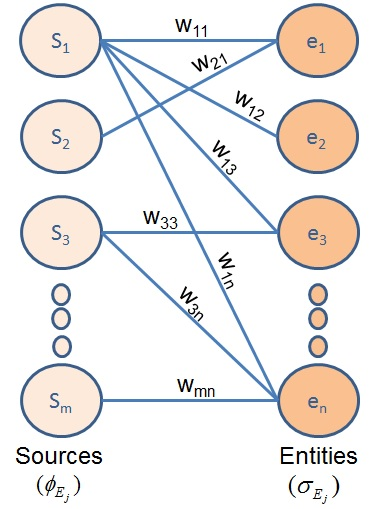
\includegraphics[height=4in,width=2.8in]{Figures/Chapter3Figures/graphnew.jpg} 
\caption{\small Bipartite graph G representing the mutual relationship between the sources and the entities.} 
\label{fg:graph}
\end{figure*}

We construct a bipartite graph $G = (V, U)$ (Figure~\ref{fg:graph}) representing the mutual relationship between the sources and the entities, where $V \in \phi_{E_{j}}, \sigma_{E_{j}}$, is the set of vertices for $G$, and $U$ is the set of undirected edges. The sources without entities are discarded during this process.

The presence of an entity in a source is not sufficient to determine its specificity. In order to express the specificity of a source w.r.t an event, we need to consider the closeness value of the entities present in the source. Given the closeness $\tau(e_{n})_{E_{j}}$ of an entity $e_{n}$ w.r.t an event $E_{j}$, obtained from the event dictionary, a weight $w_{mn}$ is assigned to the edges of the graph, which expresses the magnitude by which an entity is related to a source $S_{m}$.  

The significance of an entity $e_{n}$ in a source $S_{m}$ is expressed as,
\begin{equation}
\frac{f(e_{n}, S_{m})}{\displaystyle\sum\limits_{n=0}^{q} {f(e_{n}, S_{m})} }
\end{equation}

\noindent where, $f(e_{n}, S_{m})$ is the frequency of occurrence of the entity $e_{n}$ in the source $S_{m}$. Therefore mathematically,
\begin{equation}
w_{mn} = \frac{\tau(e_{n})_{E_{j}}\ast f(e_{n}, S_{m}) }{\displaystyle\sum\limits_{n=0}^{q} f(e_{n}, S_{m}) }
\end{equation}

The adjacency matrix of the bipartite graph G is denoted by L, and is defined as follows:

\[
L_{mn} = \left\{ \begin{array}{ccc}
w_{mn} & ~~ & if\  (m,n)\in U \\\\
0 & ~~ & otherwise \end{array} \right.
\]

%\noindent where, \textit($w_{mn}$) is the edge weight connecting source m and entity n. Mathematically,
%
%\begin{equation}
%w_{mn} = \frac{\tau_{E_{je_{n}}}\ast e{f_{mn}}}{\displaystyle\sum\limits_{n=0}^{q} e{f_{mn}} }
%\end{equation}
%
%\noindent where, $\tau_{E_{je_{n}}}$ is the closeness score of the entity $e_{n}$, obtained from the event dictionary (Section \ref{eventdict}) for the event $E_{j}$. . $\tau_{E_{je_{n}}}$ measures the significance of the entity w.r.t the event $E_{j}$ and the portion $\frac$



%\framebox{


%\squeezeup
%\begin{figure}[htbp]
%\begin{center}
%
%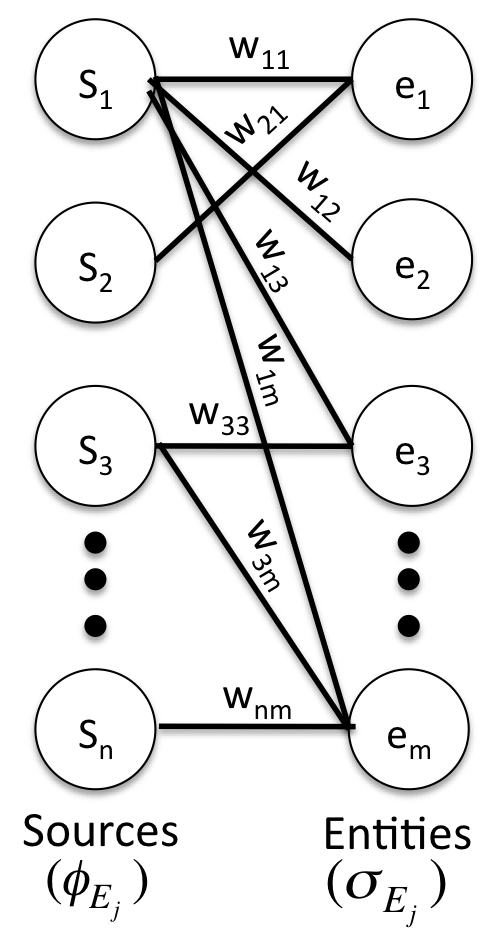
\includegraphics[height=3in,width=1.5in]{Figures/graph.jpg} 
%\caption{\small Source-entity graph for event $E_{j}$.} 
%\label{fg:figure1}
%
%\end{center}
%\end{figure}

\begin{figure}[htb]
\begin{center}

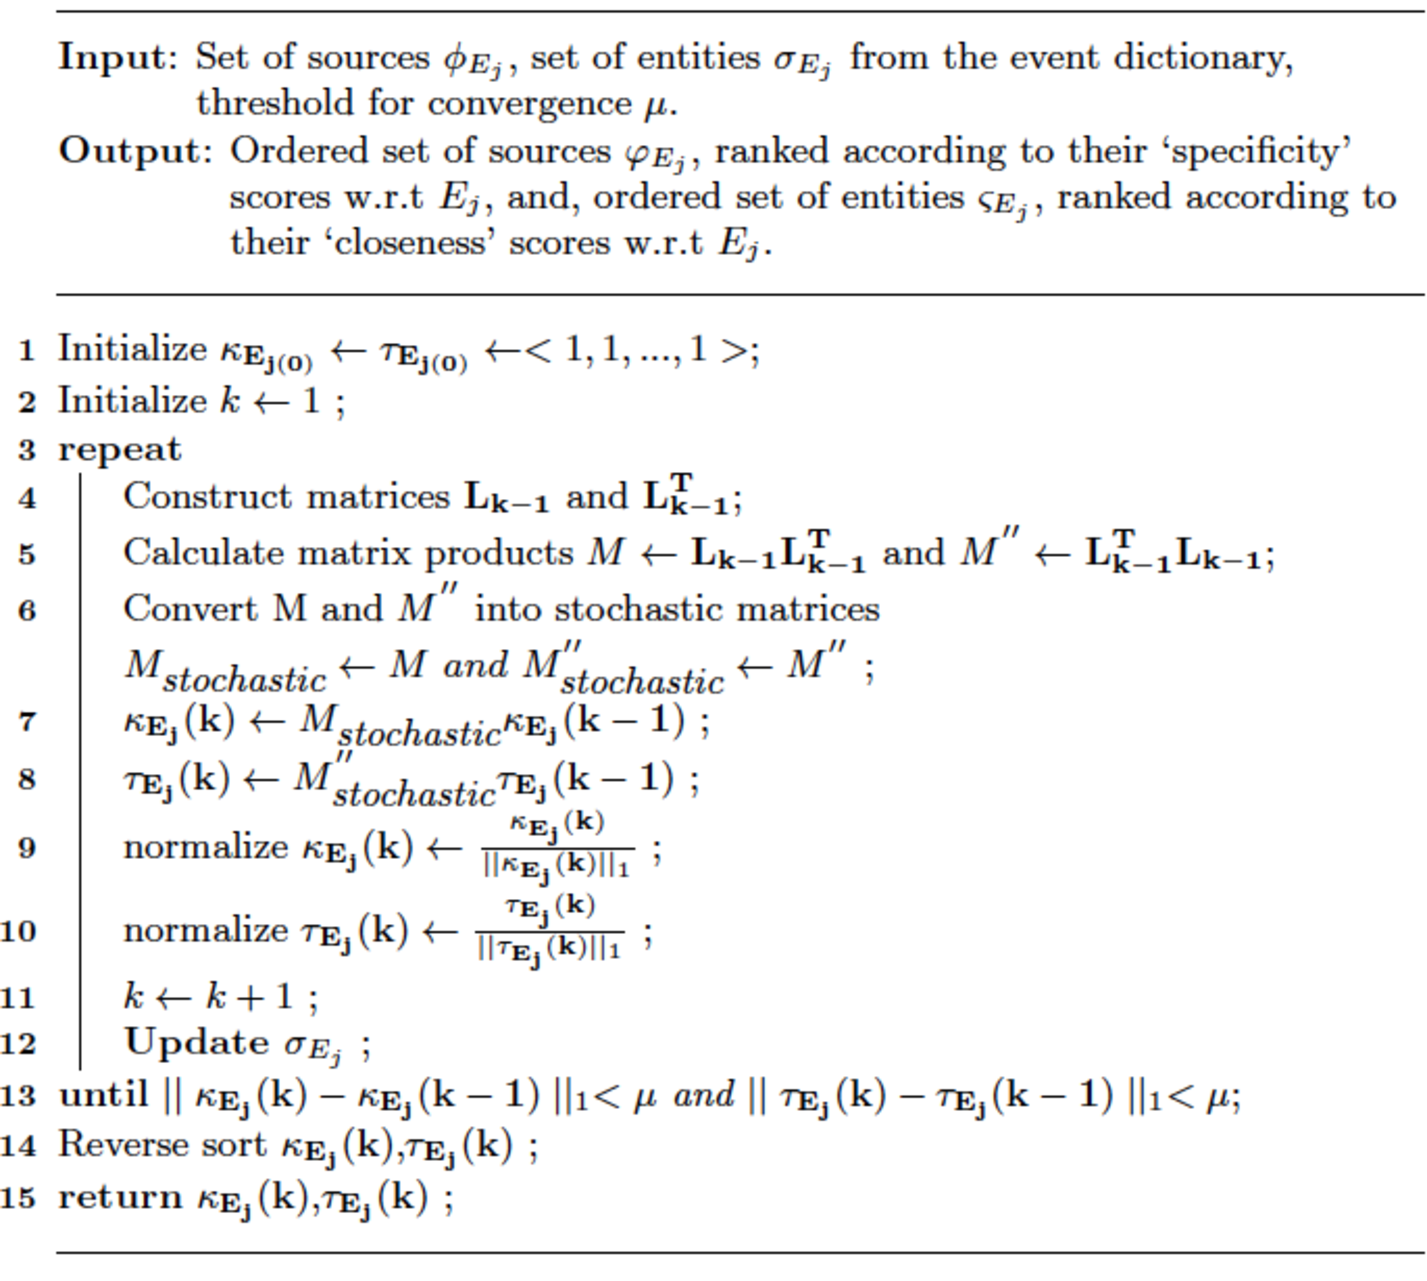
\includegraphics[height=4in,width=4.5in]{Figures/Chapter3Figures/algo.pdf} 
\caption{\small Algorithm for calculating `specificity' and `closeness'.} 
\label{fg:algo}
\end{center}
\end{figure}




Following the Mutual Reinforcement Principle the relationships between specificity scores of sources and closeness scores of entities for event $E_{j}$ can be denoted as follows,
\begin{equation}
\label{eq3}
\mathbf{\kappa_{E_{j}}} = \mathbf{L}\mathbf{\tau_{E_{j}}} 
\end{equation}


\begin{equation}
\label{eq4}
\mathbf{\tau_{E_{j}}} = \mathbf{L^{T}}\mathbf{\kappa_{E_{j}}}
\end{equation}

\noindent Substituting the values for $\mathbf{\kappa_{E_{j}}}$ and $\mathbf{\tau_{E_{j}}}$, we derive the following equations,
\begin{equation}
\label{eq5}
\mathbf{\kappa_{E_{j}}} = \mathbf{LL^{T}}\mathbf{\kappa_{E_{j}}} 
\end{equation}

\begin{equation}
\label{eq6}
\mathbf{\tau_{E_{j}}} = \mathbf{L^{T}L}\mathbf{\tau_{E_{j}}}
\end{equation}

\noindent Equations \ref{eq5} and \ref{eq6} are characteristic equations of an eigensystem, where the solutions to $\mathbf{\kappa_{E_{j}}}$  and $\mathbf{\tau_{E_{j}}}$ are the respective eigen vectors with the corresponding eigenvalue of 1. 

To emphasize the relationship between the sources and the entities, we make a major contribution by modifying the way the equations \ref{eq5} and \ref{eq6} are solved. We make the matrices $\mathbf{LL^{T}}$ and $\mathbf{L^{T}L}$ evolutionary while solving the equations. Since each of the equations is a circular definition, the final specificity and closeness scores are computed using the power iteration method \cite{golub1996matrix}. Each iteration improves specificity and closeness scores reflecting their mutual relationship. As we move towards getting the specific sources and close entities in each iteration, we update the weights $(w_{mn})$ assigned to the edges between the sources and the entities by the newly calculated closeness scores for the entities. This results in renewed reinforcement of the relationship at every iteration  by getting closer entities from better sources and vice-versa. This essentially helps the model incorporate the newly discovered knowledge about the events. More precisely, the improved understanding of the relationship between the source and the entities vis-a-vis an event is incorporated into the model.



The updation of the edge weights and the matrices with $k^{th}$ iteration is represented as follows,

\begin{equation}
w_{mn(k)} = \frac{\tau(e_{n\mathbf{(k-1)}})_{E_{j}}\ast f(e_{n}, S_{m})}{\displaystyle\sum\limits_{n=0}^q f(e_{n}, S_{m})} 
\end{equation}


\[
L_{mn(k)} = \left\{ \begin{array}{ccc}
w_{mn(k)} & ~~ & if\  (m,n) \in U \\\\
0 & ~~ & otherwise \end{array} \right.
\]

\noindent where, $L_{mn(k)}$ represents the adjacency matrix for graph G, and $w_{mn(k)}$ denotes the edge weight for the edge between $m^{th}$ source and $n^{th}$ entity at the $k^{th}$ iteration. $\tau(e_{n\mathbf{(k-1)}})_{E_{j}}$ represents the closeness score of the entity $e_{n} $ w.r.t the event $E_{j} (\in \xi)$, obtained from the evolving event dictionary for event $E_{j}$ at $(k-1)^{th}$ iteration.

If, $\mathbf{\kappa_{E_{j}}(k)}$ and $\mathbf{\tau_{E_{j}}(k)}$ be the specificity and the closeness scores, at the $k^{th}$ iteration, the iterative process for generating the final solution are,

\begin{equation}
\label{eq1}
\mathbf{\kappa_{E_{j}}(k)} = \mathbf{L_{k-1}L^{T}_{k-1}}\mathbf{\kappa_{E_{j}}(k-1)} 
\end{equation}

\begin{equation}
\label{eq2}
\mathbf{\tau_{E_{j}}(k)} = \mathbf{L^{T}_{k-1}L_{k-1}}\mathbf{\tau_{E_{j}}(k-1)}
\end{equation}

In order to get 1 as the largest eigenvalue and, $\mathbf{\kappa_{E_{j}}} $ and $\mathbf{\tau_{E_{j}}}$ as the principal eigen vectors, the matrices $\mathbf{L_{k-1}L^{T}_{k-1}}$ and $\mathbf{L^{T}_{k-1}L_{k-1}}$ needs to be stochastic and irreducible \cite{langville2004deeper} at every step of our evolutionary process.  In the present case, since the graph G is a bipartite graph, matrices $\mathbf{L_{k-1}L^{T}_{k-1}}$ and $\mathbf{L^{T}_{k-1}L_{k-1}}$ are already irreducible.



%If the matrices $\mathbf{LL^{T}}$ and $\mathbf{L^{T}L}$ are stochastic and irreducible \cite{langville2004deeper} then 1 would be the largest eigenvalue and the  vectors $\mathbf{\kappa_{E_{j}}} $ and $\mathbf{\tau_{E_{j}}}$ would be the principal eigen vectors respectively. In the present case, since the graph G is a bipartite graph, matrices $\mathbf{\kappa_{E_{j}}} $ and $\mathbf{\tau_{E_{j}}}$ are already irreducible.




In order to make the matrices $\mathbf{L_{k-1}L^{T}_{k-1}}$ and $\mathbf{L^{T}_{k-1}L_{k-1}}$ stochastic, we take the following steps at each iteration,


\begin{itemize}
  \item Dividing the non-zero entries of the matrices  $\mathbf{L_{k-1}L^{T}_{k-1}}$ and $\mathbf{L^{T}_{k-1}L_{k-1}}$ by the summation of all the entries in a row. 


  \item Assigning $1/n$ to the zero entries of $\mathbf{L_{k-1}L^{T}_{k-1}}$ and $1/m$ to the zero entries of $\mathbf{L^{T}_{k-1}L_{k-1}}$, respectively.
\end{itemize}

\noindent The whole process is presented as an algorithm as shown in Fig \ref{fg:algo}.

\noindent 
We also perform our study using conventional binary static matrices represented as follows,


\[
L_{mn} = \left\{ \begin{array}{ccc}
1 & ~~ & if\  (m,n) \in U \\\\
0 & ~~ & otherwise \end{array} \right.
\]

The proposed evolutionary model outperforms the static model as validated by the results discussed in Section \ref{exp}.


%\begin{equation}
%\frac{\tau_{E_{je_{n\mathbf{(k)}}}}\ast e{f_{mn}}}{\displaystyle\sum\limits_{n=0}^q e{f_{mn}} } = \frac{\tau_{E_{je_{n\mathbf{(k-1)}}}}\ast e{f_{mn}}}{\displaystyle\sum\limits_{n=0}^q e{f_{mn}} } 
%\end{equation}

%\begin{equation}
%\mathbf{w_{(k)}} = \mathbf{w_{(k-1)}}
%\end{equation}







\section{\label{data} \textbf{Data Collection}}
\noindent \textbf{\textit{Motivation behind source selection:}} For many people blogs have become popular social media sources for satisfying interpersonal communication needs. Blogs act as a platform for masses to share their likes and dislikes, voice their opinions, provide suggestions and report news. Over the years blogging has matured from personal diaries to citizen journalistic sources providing live coverage of events beyond the professional newsrooms. Often mainstream media rely on blogs for reporting first-hand accounts of an event \cite{ekdale2007expression}. Other social media platforms like microblogs, social networks etc., also promote such activities. But, these platforms have very little scope to elaborately discuss about the events due to the limitations in the length of content allowed to be posted. However, these alternative platforms act as good sources for studying and tracking dissemination of information during real-life events. This motivated us to perform our experiments on sources collected from the blogging platforms instead of other social media websites.

\begin{table}[htbp]
\centering
\caption{Details of Data Collected.}
\label{tab:table1}
\begin{tabular}{|c|c|c| }
\hline
\textbf{Service Used} & \textbf{Event} & \textbf{Number of Blog Posts} \\ [0.5ex]
\hline
GlobalVoices & Egyptian Revolution & 234 \\
&Libyan Revolution & 86 \\
&Tunisian Revolution & 77\\
\hline 
Google Blogger & Egyptian Revolution & 579 \\
&Libyan Revolution & 600 \\
&Tunisian Revolution & 484 \\
\hline
Icerocket Blog Search & Egyptian Revolution & 5900 \\ 
&Libyan Revolution & 2198 \\
&Tunisian Revolution & 1220 \\
\hline
\end{tabular}
\end{table}

%The blog writers, also known as bloggers, loosely form their special interest communities where they debate and discuss issues, spread awareness, gather support, organize and mobilize campaigns - utilizing and in many ways demonstrating the democratic nature of the Internet. 


\paragraph
\noindent \textit{\textbf{Sources:}} Blog posts from GlobalVoices, Blogger\footnote{http://blogger.com} and Icerocket Blog Search\footnote{http://icerocket.com} respectively, are collected for the study. The details of the dataset used is given in Table ~\ref{tab:table1}. The dataset includes 11,378 blog posts from various blogging platforms like blogspot.com, wordpress.com, livejournal.com, typepad.com, etc. We also filter out the non-english blogs. The data from GlobalVoices is used for constructing event dictionaries ($\sigma_{E_{j}}$), as explained in Section \ref{method}. We collect blog posts related to the three events from Blogger using Google Search, and from other blogging platforms using Icerocket blog search. We perform our experiments on the sources ($\phi_{E_{j}}$) retrieved by the search engines due to the lack of ground truth and take the sources along with the ranks assigned to them by the search engines as our baseline (explained in Subsection \ref{basecomp}) The collected blog posts are parsed for extracting various information. However, we use the following information for our study: \textit{URL} of the blog and blogpost), \textit{blog text}, \textit{entities}, \textit{language}, and \textit{rank} of the post in the respective search engines used for collecting it. We use AlchemyAPI in order to extract entities. These datasets would be made available on request.













\section{\label{exp}\textbf{Experiment and Analysis}}



In this section, we describe the experiments performed. First, we discuss the experimental setup, followed by the comparative analysis between the proposed evolutionary mutual reinforcement model and conventional mutual reinforcement model. We then, introduce a novel evaluation strategy comparing the proposed model with two baseline models.
\subsection{\textbf{Experimental Setup}}
The methodology discussed earlier is implemented on the collected datasets. We take the following steps in order to perform the experiment,

\begin{itemize}
\item \textit{\textbf{Constructing the Event Dictionaries:}} We take $\xi$ = \{``Egyptian Revolution", ``Libyan Revolution", ``Tunisian Revolution"\} as our set of events. We construct the event dictionaries ($\sigma_{E_{j}}$) by using the sources from GlobalVoices (explained in Event Dictionary subsection). 

%\item The sources related to each of these events are collected from Google and Icerocket as explained in Data Collection section.

%The $\tau(e_{i})_{E_{j}}$ values of the entities are calculated. The distribution of $\tau(e_{i})_{E_{j}}$ scores of entities for the set of events is presented in Figure 6. The threshold values ($\alpha_{E_{j}}$) for each event $E_{j} \in \xi$ are decided after careful manual inspection for constructing the event specific-dictionaries.

\item \textit{\textbf{Implementing the Proposed Evolutionary Mutual Reinforcement Model:}} The algorithm, as presented in Figure \ref{fg:algo}, is implemented on the set of sources ($\phi_{E_{j}}$) from Blogger and Icerocket related to each event respectively, and the set of entities ($\sigma_{E_{j}}$) from the event dictionary corresponding to each event $E_{j}$. The threshold value for convergence $\mu$ is set to 1e-08.

%
% We perform our experiment on the sources retrieved by the search engines due to the lack of baselines (explained in the Baseline Comparisons subsection). 

\item \textit{\textbf{Obtaining Specific Sources and Close Entities:}} With the termination of the algorithm we get a ranked set of sources ($\varphi_{E_{j}}$) ordered in terms of their specific information content and entities ($\varsigma_{E_{j}}$) ordered in terms of how closely related they are to the event. 

\item \textit{\textbf{Conventional Mutual Reinforcement Model Approach:}} We also implement the conventional mutual reinforcement model on $\phi_{E_{j}}$ and $\sigma_{E_{j}}$ without considering the evolving matrices (explained in Subsection \ref{mutual}).

\end{itemize}



%We have $\xi$ = \{``Egyptian Revolution", ``Libyan Revolution", ``Tunisian Revolution"\} as our set of events under study. Algorithm \ref{fg:algo} is implemented on the set of sources related to each event, and the set of entities from the event dictionary constructed in Section \ref{eventdict}. The threshold value for convergence $\mu$ is set to a very small value of 1e-08. We also implement algorithm \ref{fg:algo} without considering the evolving matrices, as explained in Section.
%
%With the termination of the algorithm we get a ranked set of sources ordered in terms of its specific information content and entities ordered in terms of how closely it is related to the event, as explained in Section 4. We further analyze the ranking of the top K specific sources as identified by our methodology and observe the difference in their rankings as assigned by the search engines and as assigned by our model. Figure \ref{fg:figure22} shows ranks assigned by Google and Icerocket for the top 10 sources for each event, ranked according to our framework. We conclude, that  our framework could identify the sources, which often gets buried in the Long Tail and has the potential for presenting valuable information about the event.





%\begin{figure*}[htbp]
%\begin{center}$
%\begin{array}{ccc}
%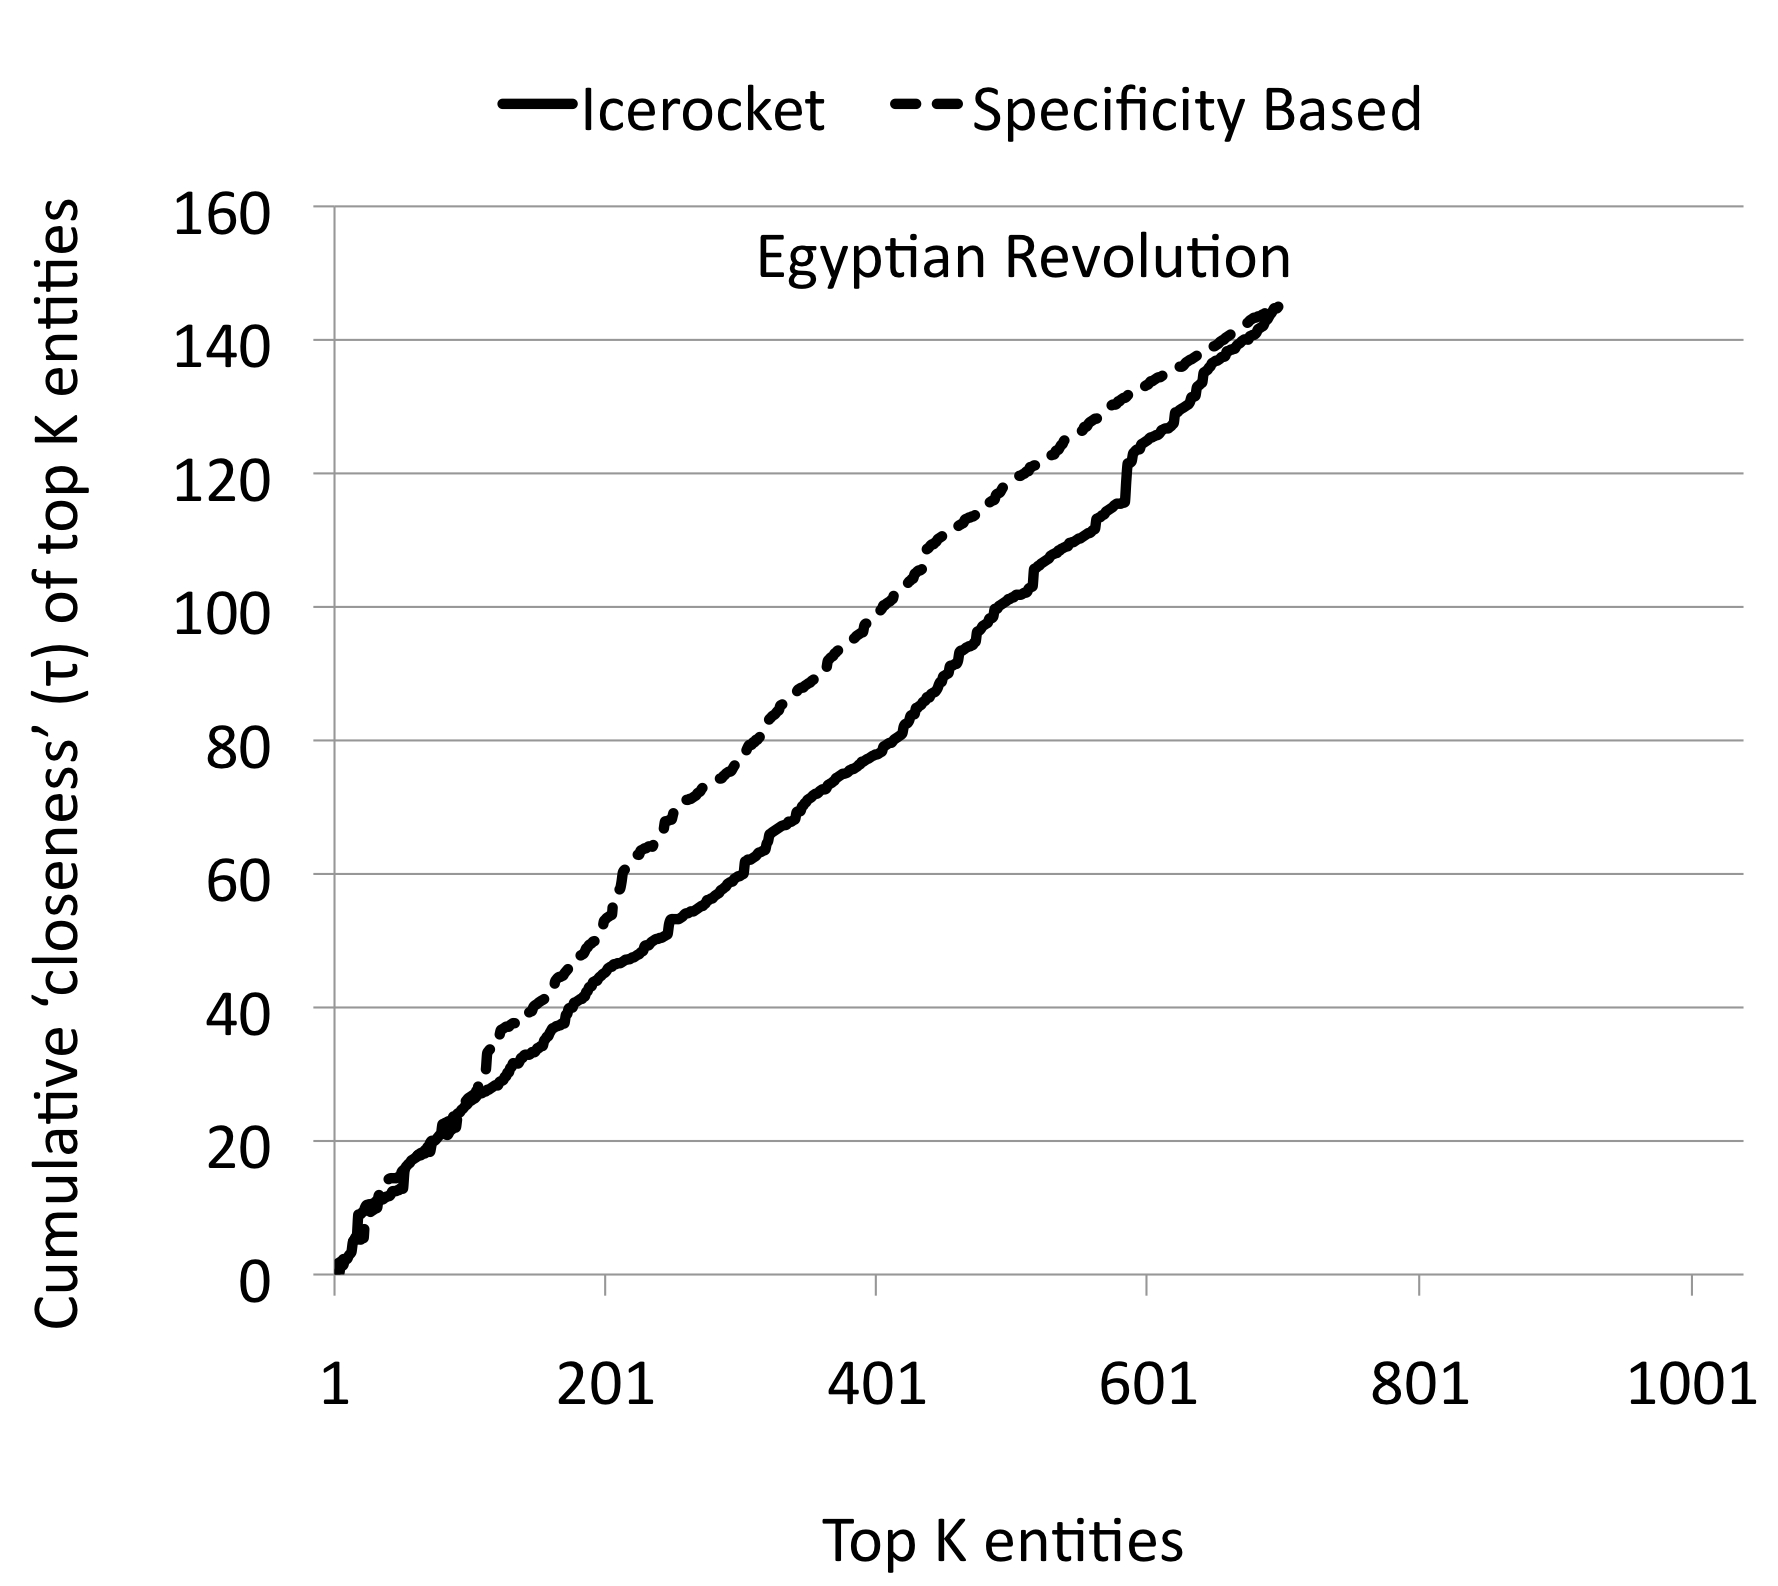
\includegraphics[height=2in,width=2in]{Figures/EgyptCumulativeIcerocket.jpg} &
%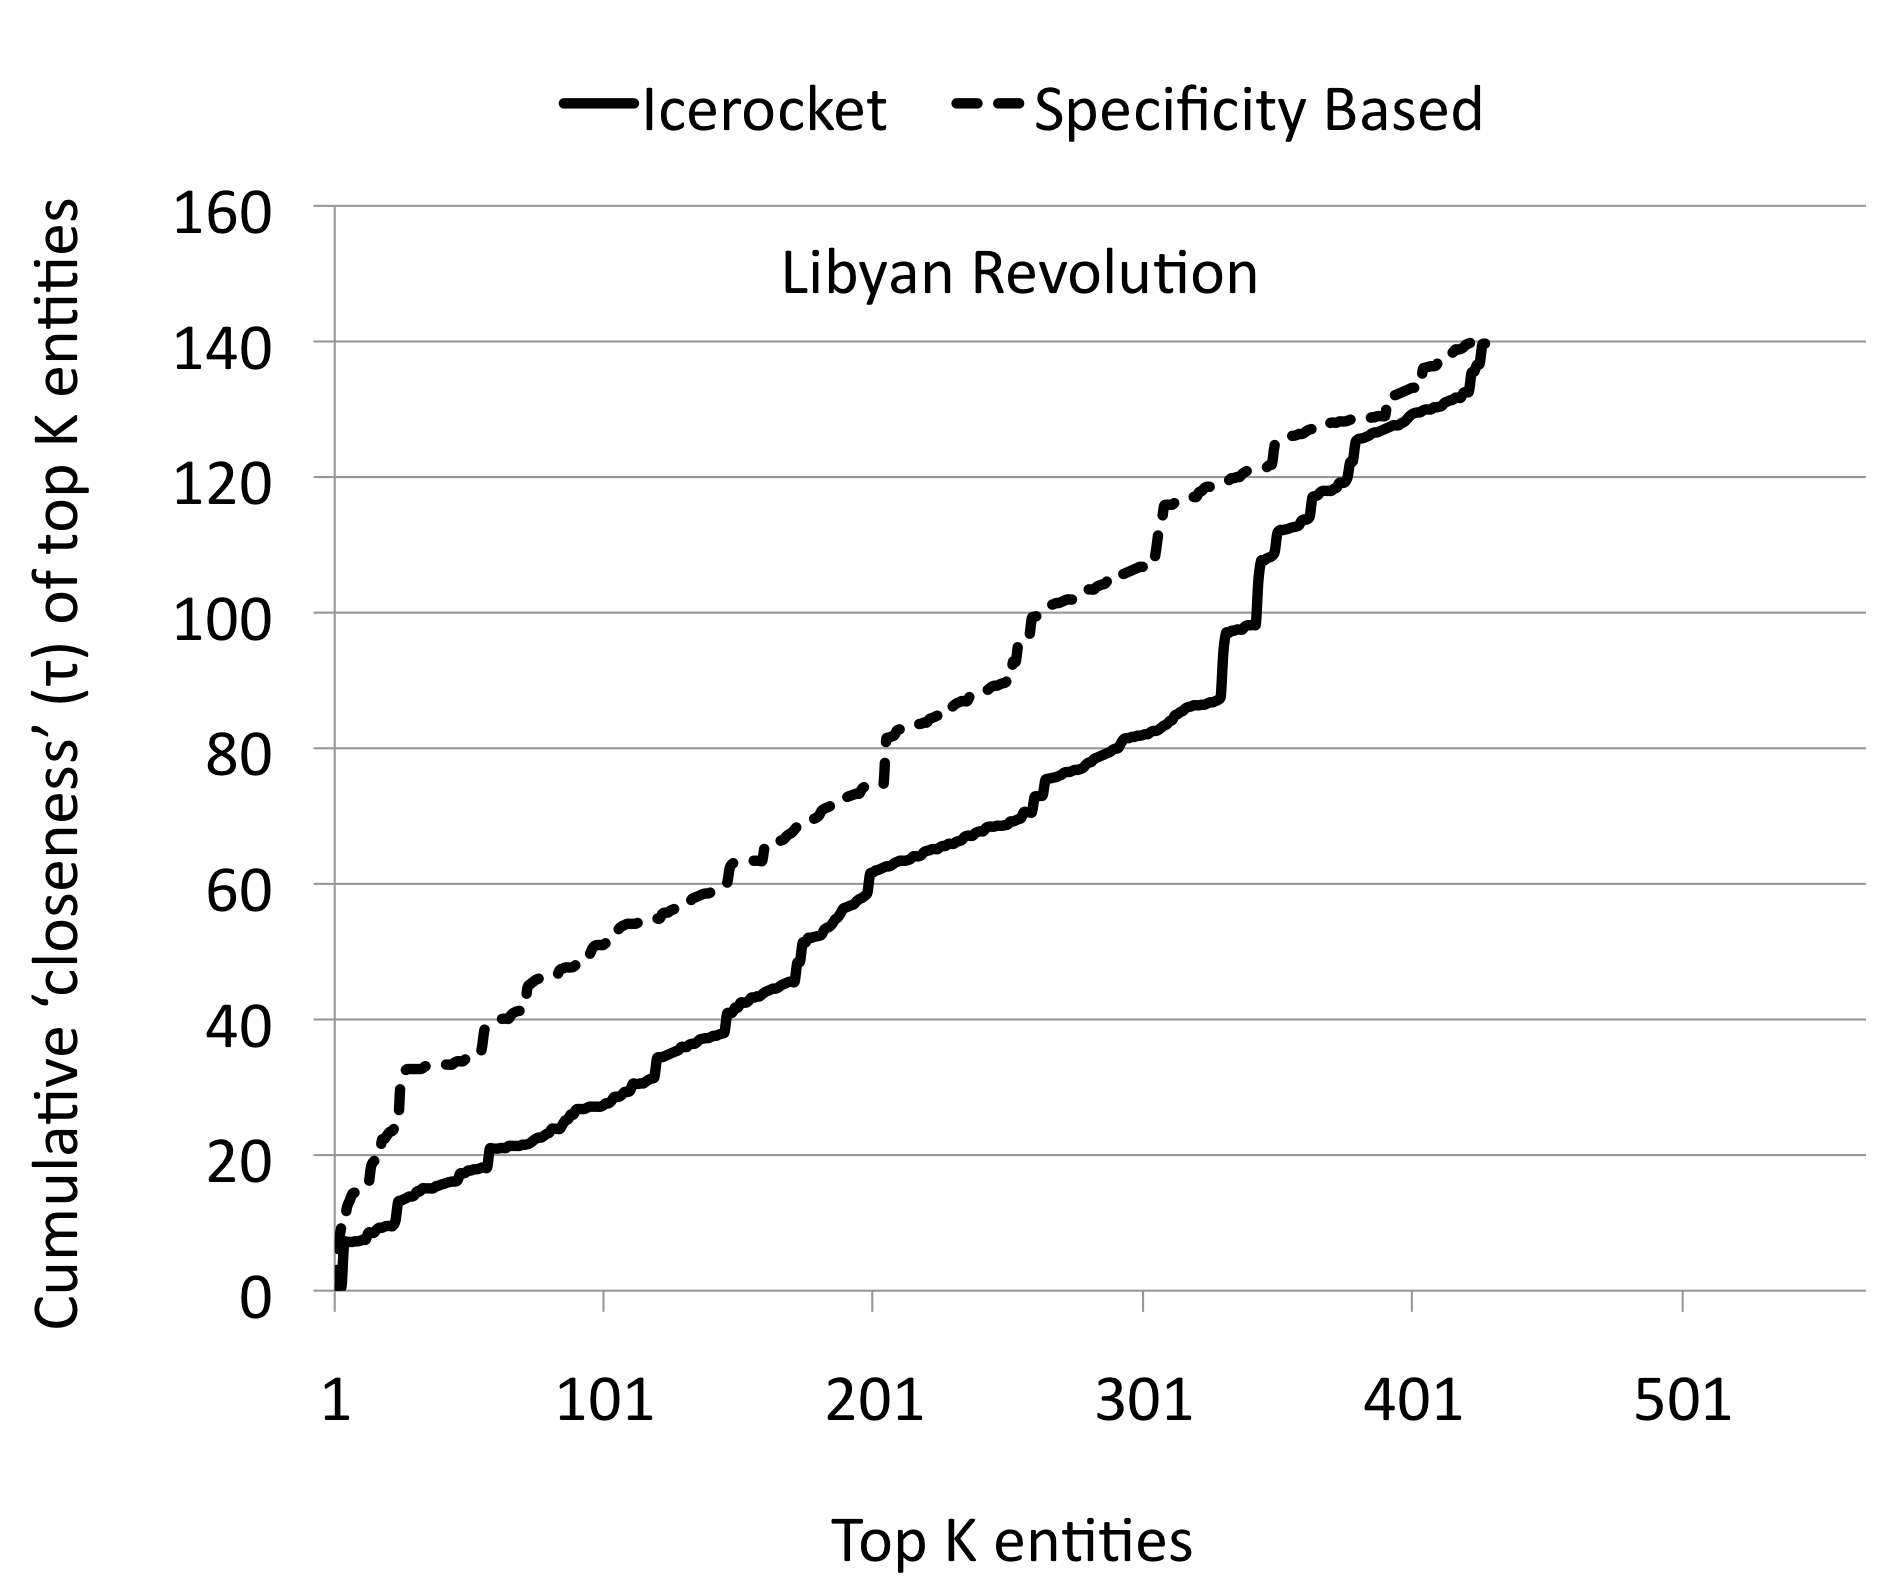
\includegraphics[height=2in,width=2in]{Figures/LibyaCumulativeIcerocket.jpg} &
%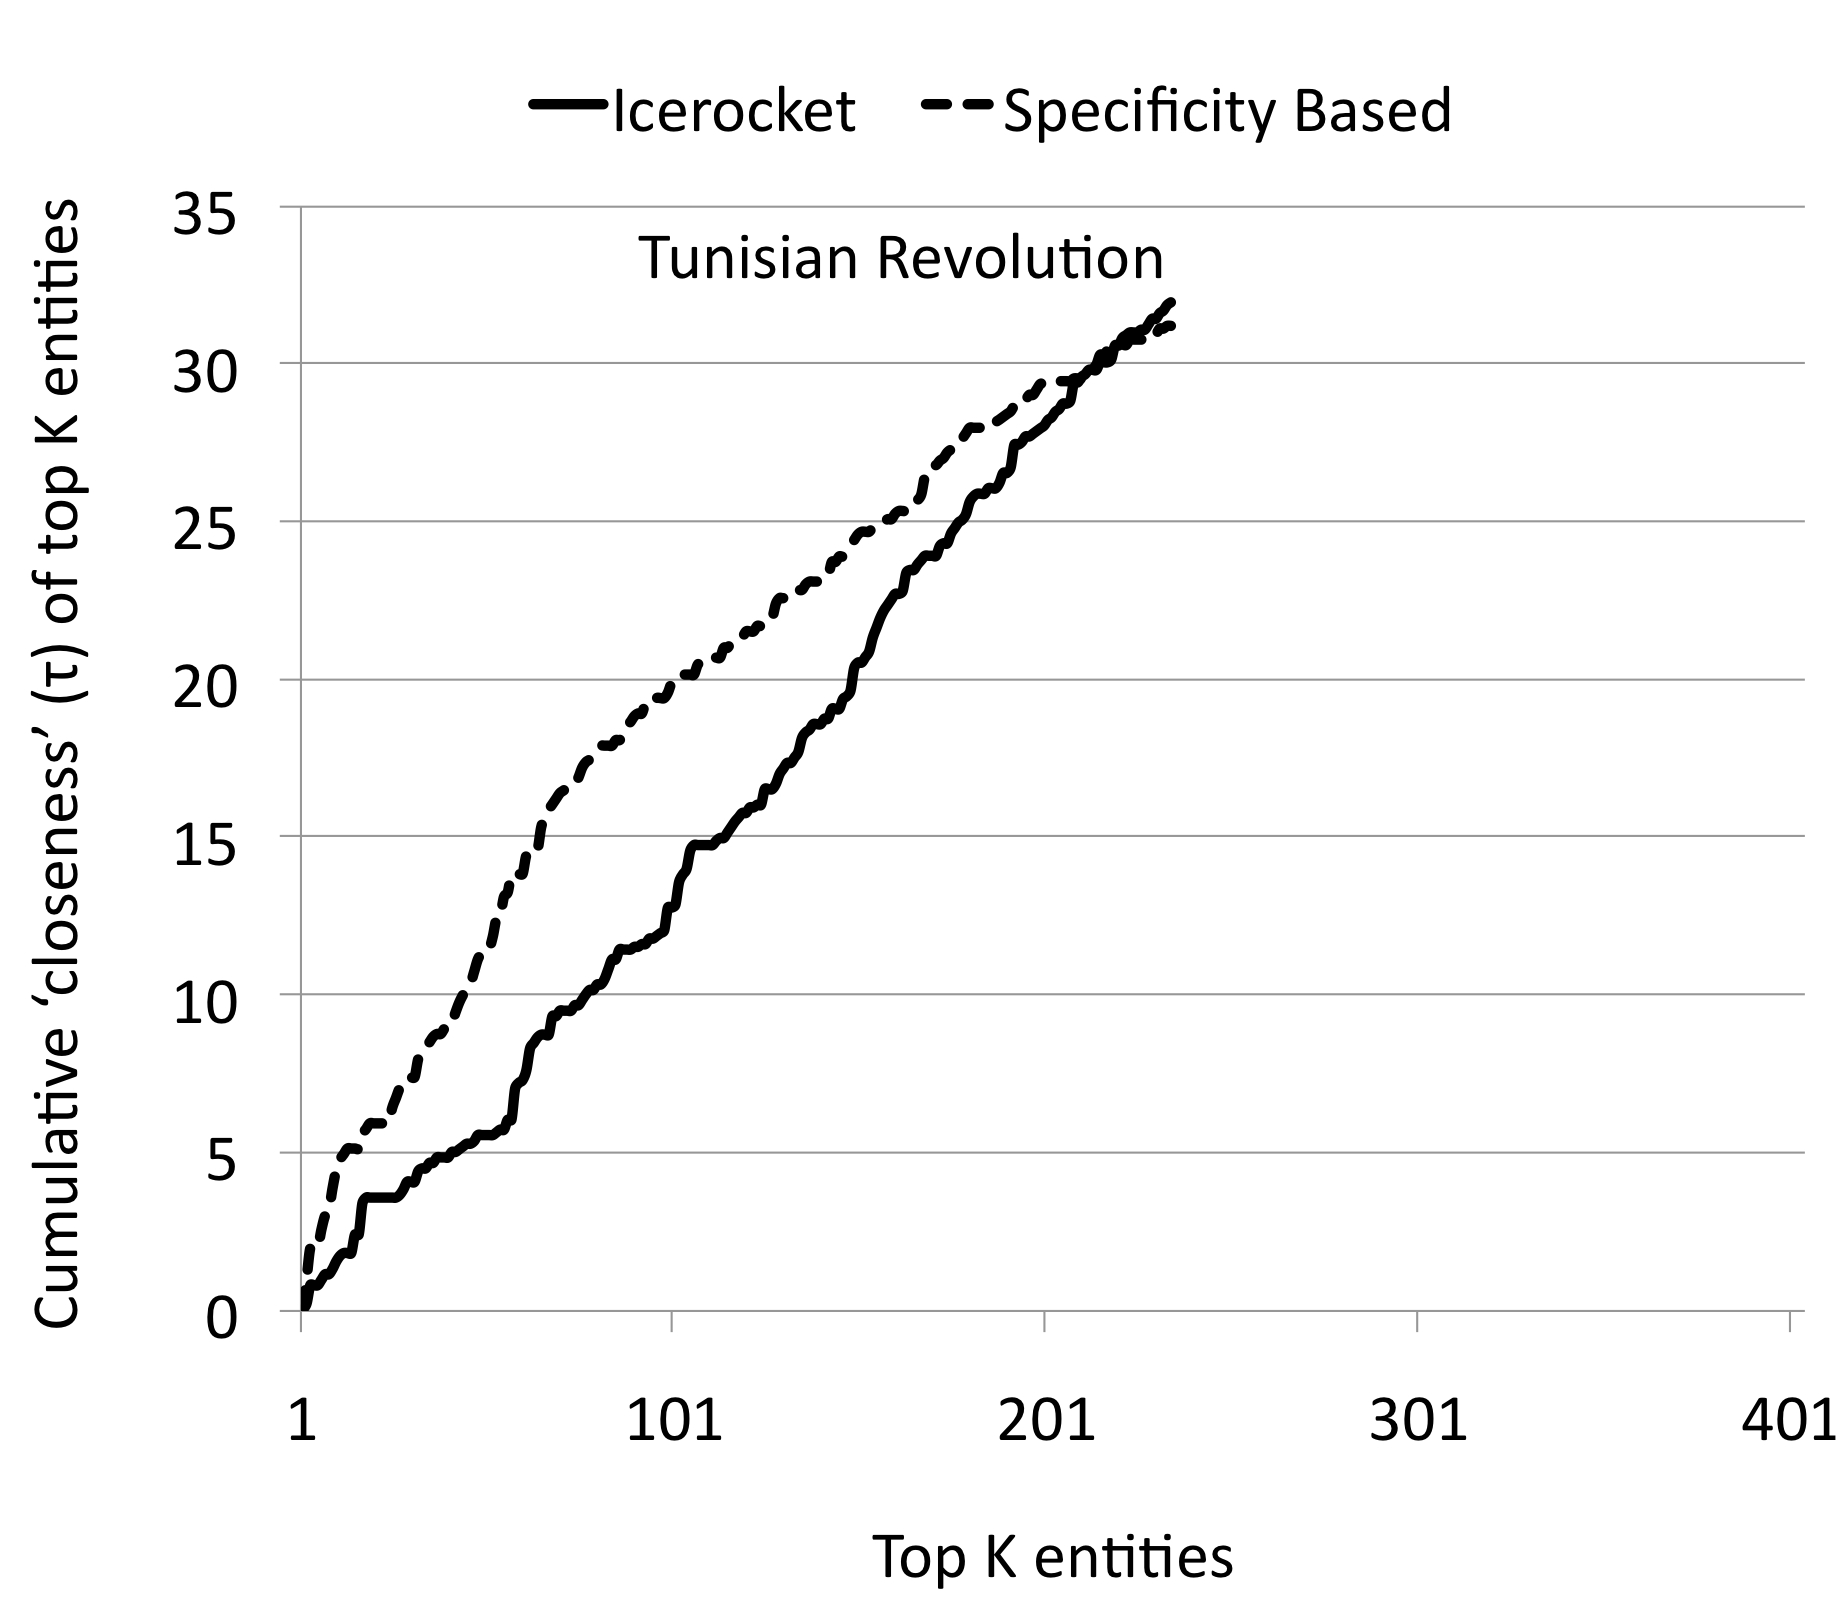
\includegraphics[height=2.2in,width=2in]{Figures/TunisiaCumulativeIcerocket.jpg}
%\end{array}$
%\end{center}
%\caption{Validating`specificity' $(\kappa)$ for sources from Icerocket Blog Search.}
%\label{fg:figure4}
%\end{figure*}


%\begin{table}[htbp]
%
%\caption{\small Top 5 entities in the event specific and the event class dictionaries constructed for the set of events $\xi$.}
%\label{tab:table2}
%\centering
%\begin{tabular}{|l|p{9cm}|}
%\hline
%\textbf{Egyptian Revolution Specific Dictionary} & Tahrir Square, Egyptian government, Gigi Ibrahim, Alexandria, Wael Abbas. \\
%\hline
%\textbf{Libyan Revolution Specific Dictionary} & Tripoli, Muammar Al Gaddafi, North Atlantic Treaty Organization, Chad, United Kingdom \\ 
%\hline
%\textbf{Tunisian Revolution Specific Dictionary} & Tunisian government, Lin Ben Mhenni, Samir Feriani, Kasbah Square, RCD \\ 
%\hline
%\textbf{Socio-Political event dictionary} & Twitter, Iranian Government, Tear gas devices, Facebook, Big Social network \\ 
%\hline
%
%\end{tabular}
%\end{table}



\subsection{\label{compconvevol}\textbf{Comparing Conventional and Evolutionary Mutual Reinforcement Models}}


In order to compare the efficiency of the proposed evolutionary mutual reinforcement model with the conventional mutual reinforcement model we combine the sources collected for an event $E_{j}$ from Google search and Icerocket search. After that we run the proposed evolutionary mutual reinforcement model and conventional mutual reinforcement model on the combined set of sources and event dictionary ($\sigma_{E_{j}}$) for each event. The number of iterations taken by the power iteration method to converge in each case is analyzed in Figure \ref{fg:figure12}. It is observed that the number of iterations taken by the power iteration method is lesser, when we employ the evolutionary mutual reinforcement model. Hence, we observe a marked improvement in the performance of our evolutionary mutual reinforcement model over the conventional static mutual reinforcement model.

\begin{figure}[htbp]
\centering
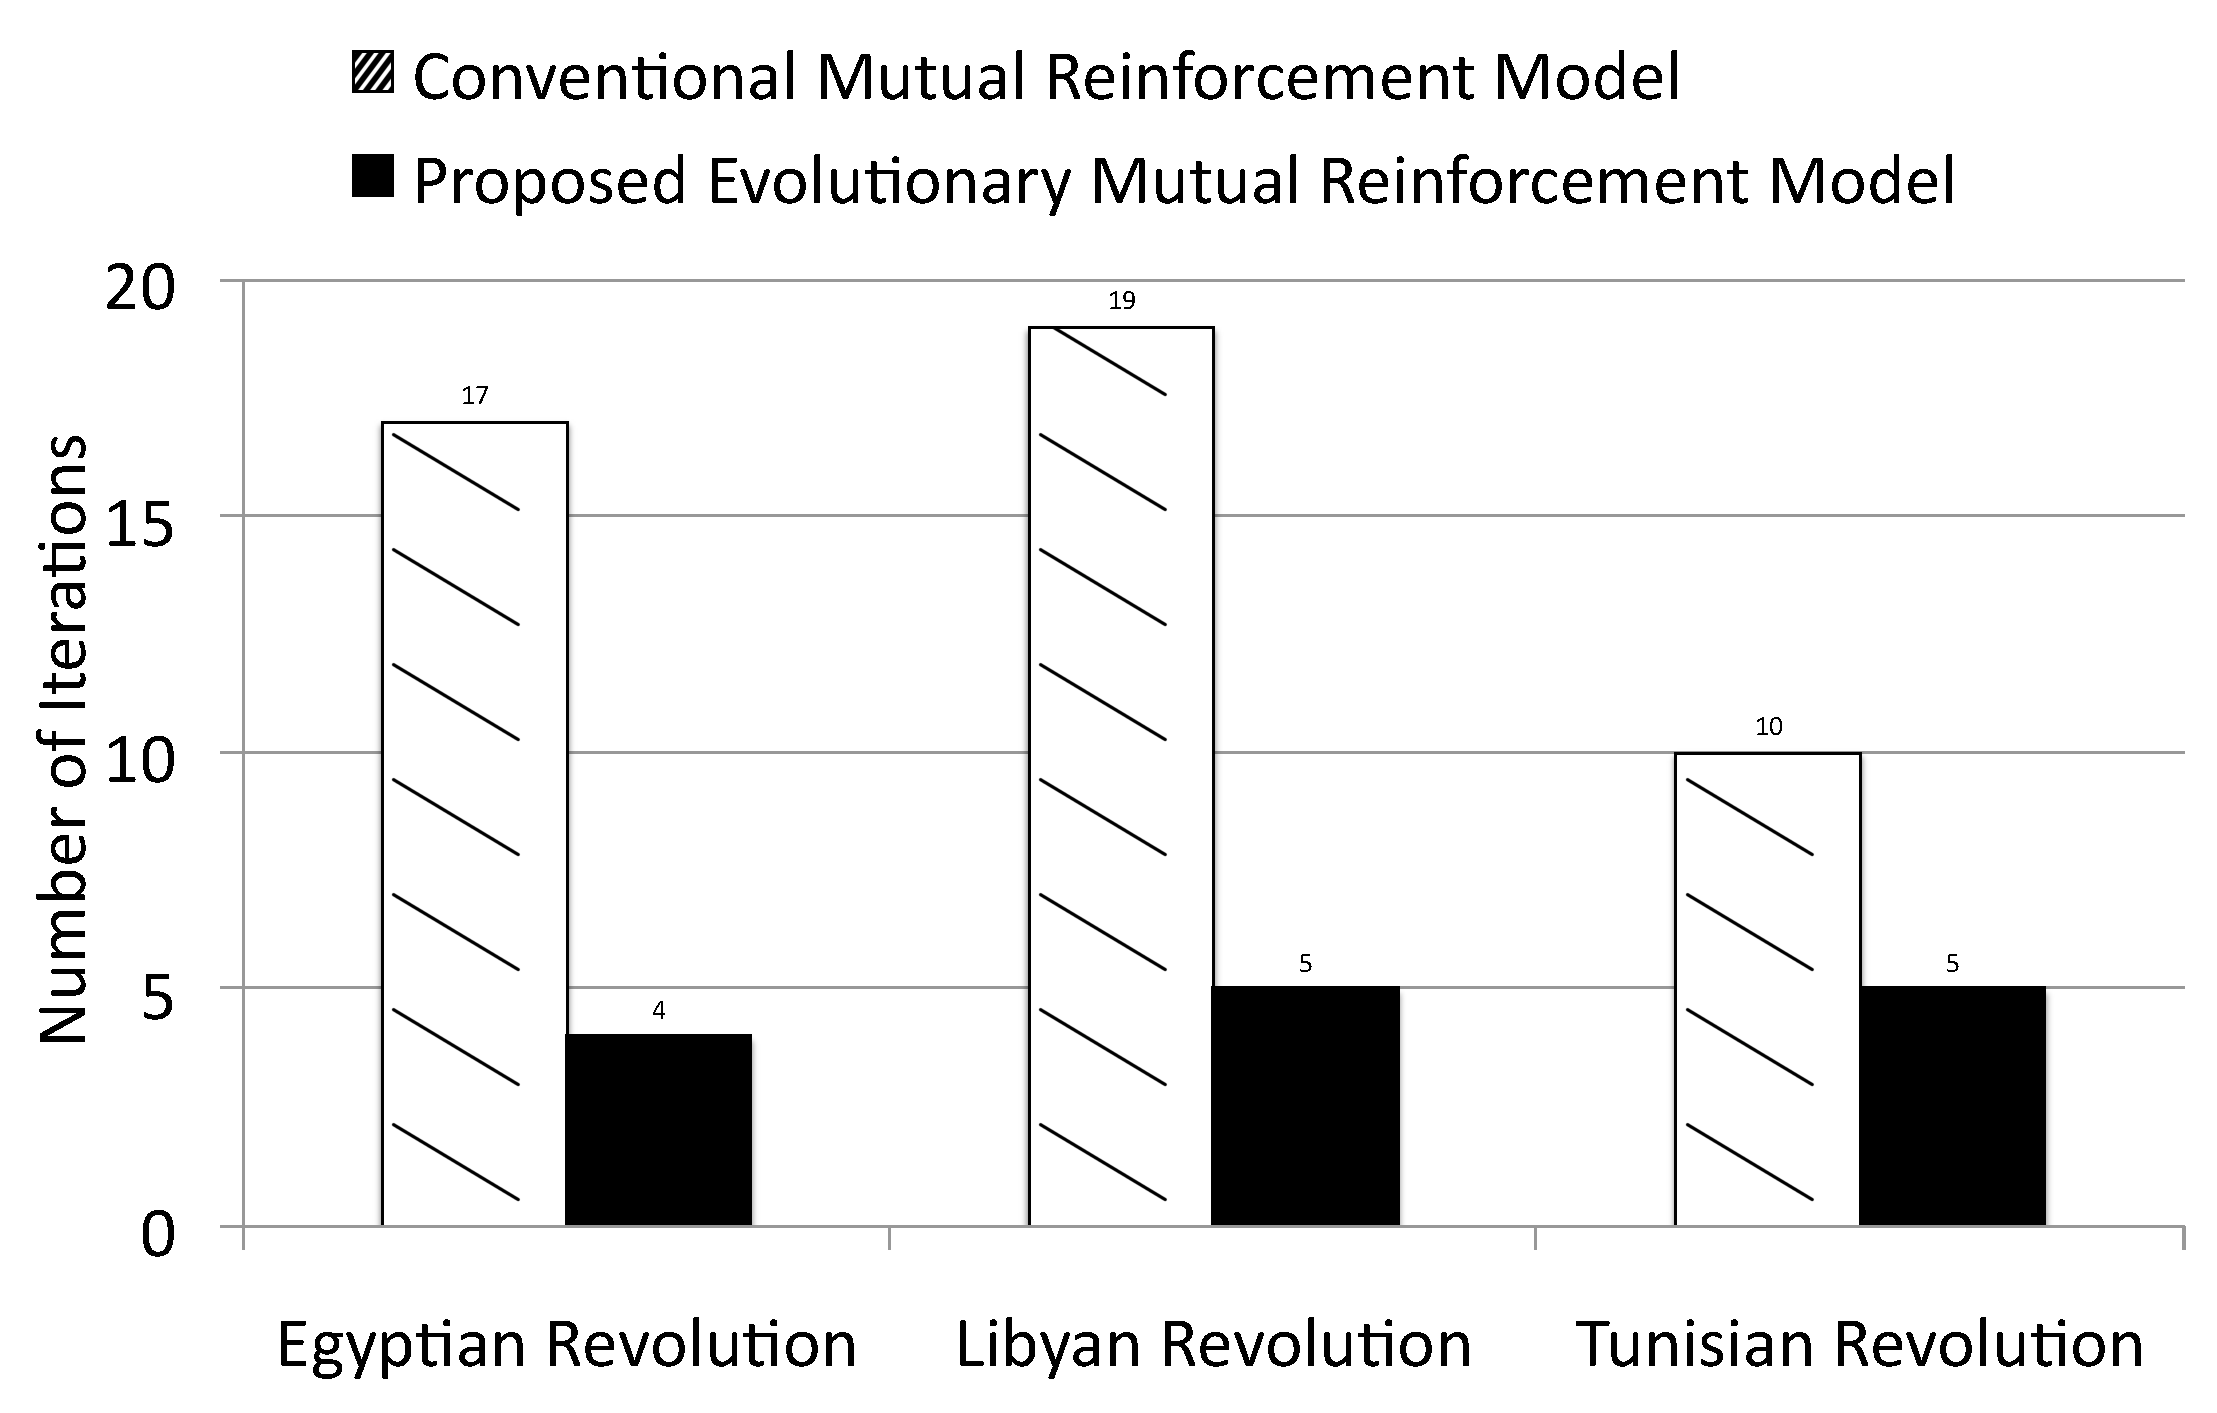
\includegraphics[height=2.5in,width=3in]{Figures/Chapter3Figures/Iteration.pdf}

\caption{\small Comparison of number of iterations taken by the power iteration method to converge, for the set of sources related to events in $\xi$, with the proposed evolutionary mutual reinforcement model and the conventional static mutual reinforcement model.}
\label{fg:figure12}

\end{figure}

\noindent \textit{\textbf{Explanation for the improvement:}} The lesser number of iterations in the proposed evolutionary mutual reinforcement model can be explained by the introduction of the evolutionary weights assigned to the relationship between the sources and the entities. The improved closeness scores ($\tau(e_{i},E_{j}$)) at each iteration of the evolutionary model and the renewed reinforcement of the relationship between the entities and the sources decreases the number of iterations taken by the proposed evolutionary model to converge in comparison to the static conventional model. Next, we compare the performance of the proposed evolutionary model with the baselines and the conventional mutual reinforcement model in terms of how quickly the models help in identifying valuable information about the events.

\begin{figure*}[htb]
\centering$
\begin{array}{c}
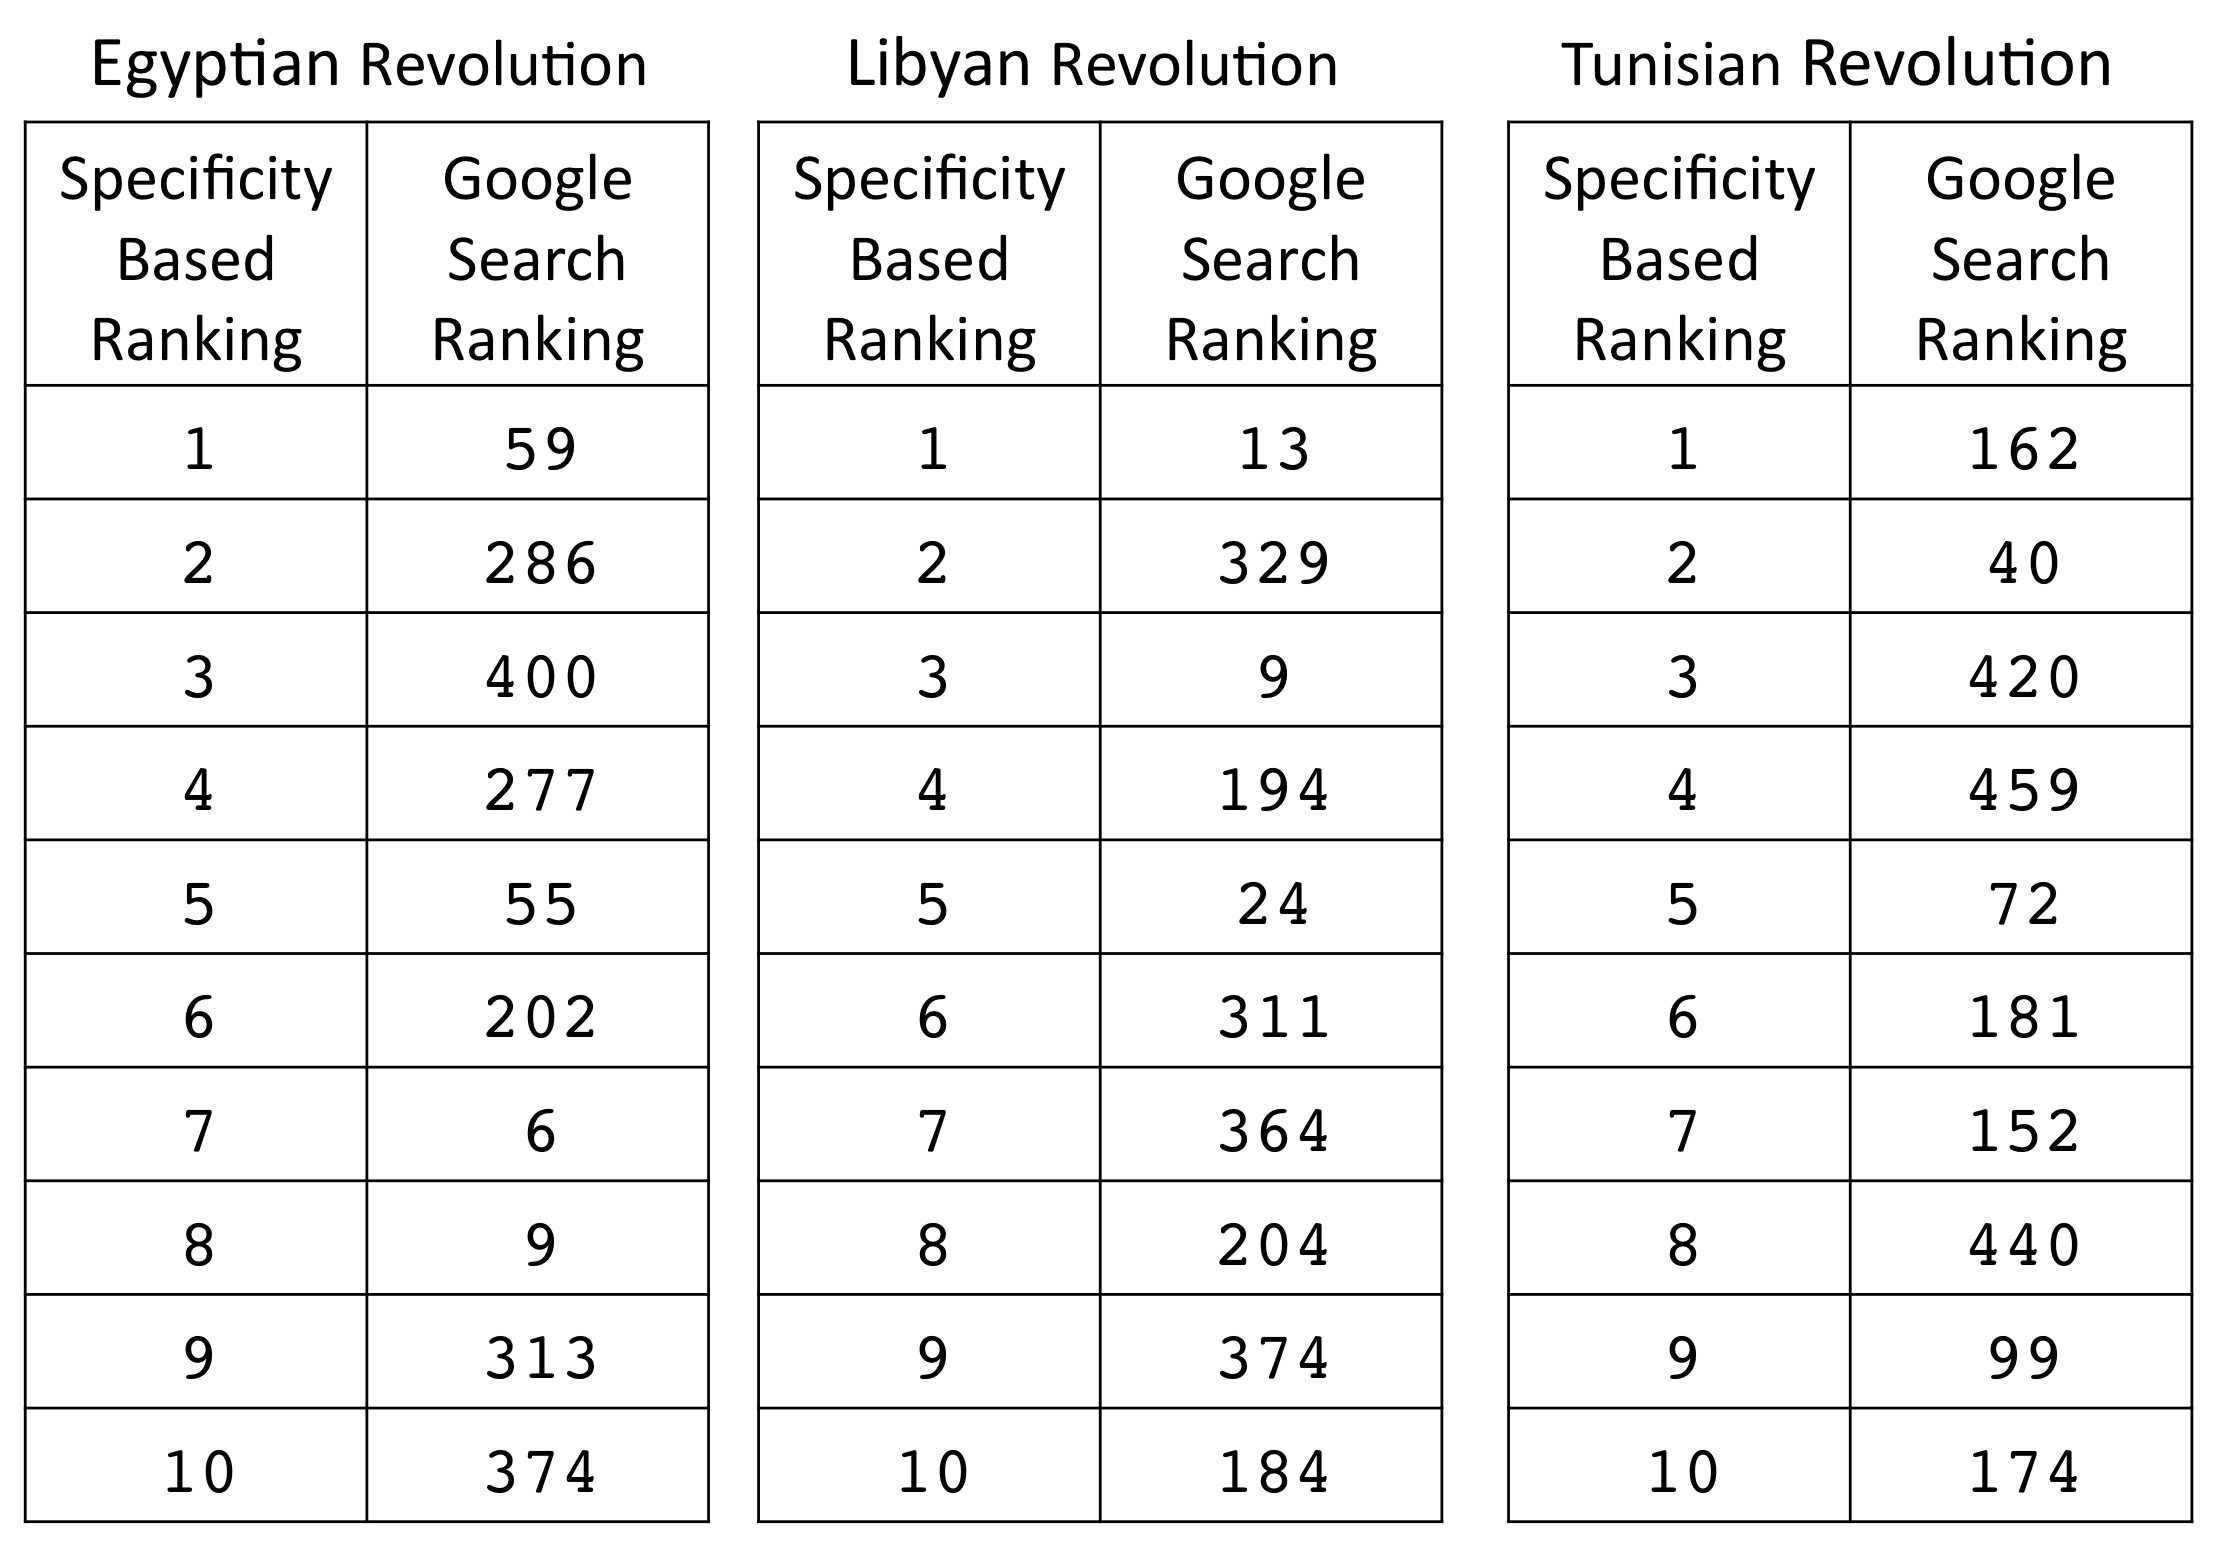
\includegraphics[height=2in,width=3.5in]{Figures/Chapter3Figures/RankDistGoogle.jpg} \\
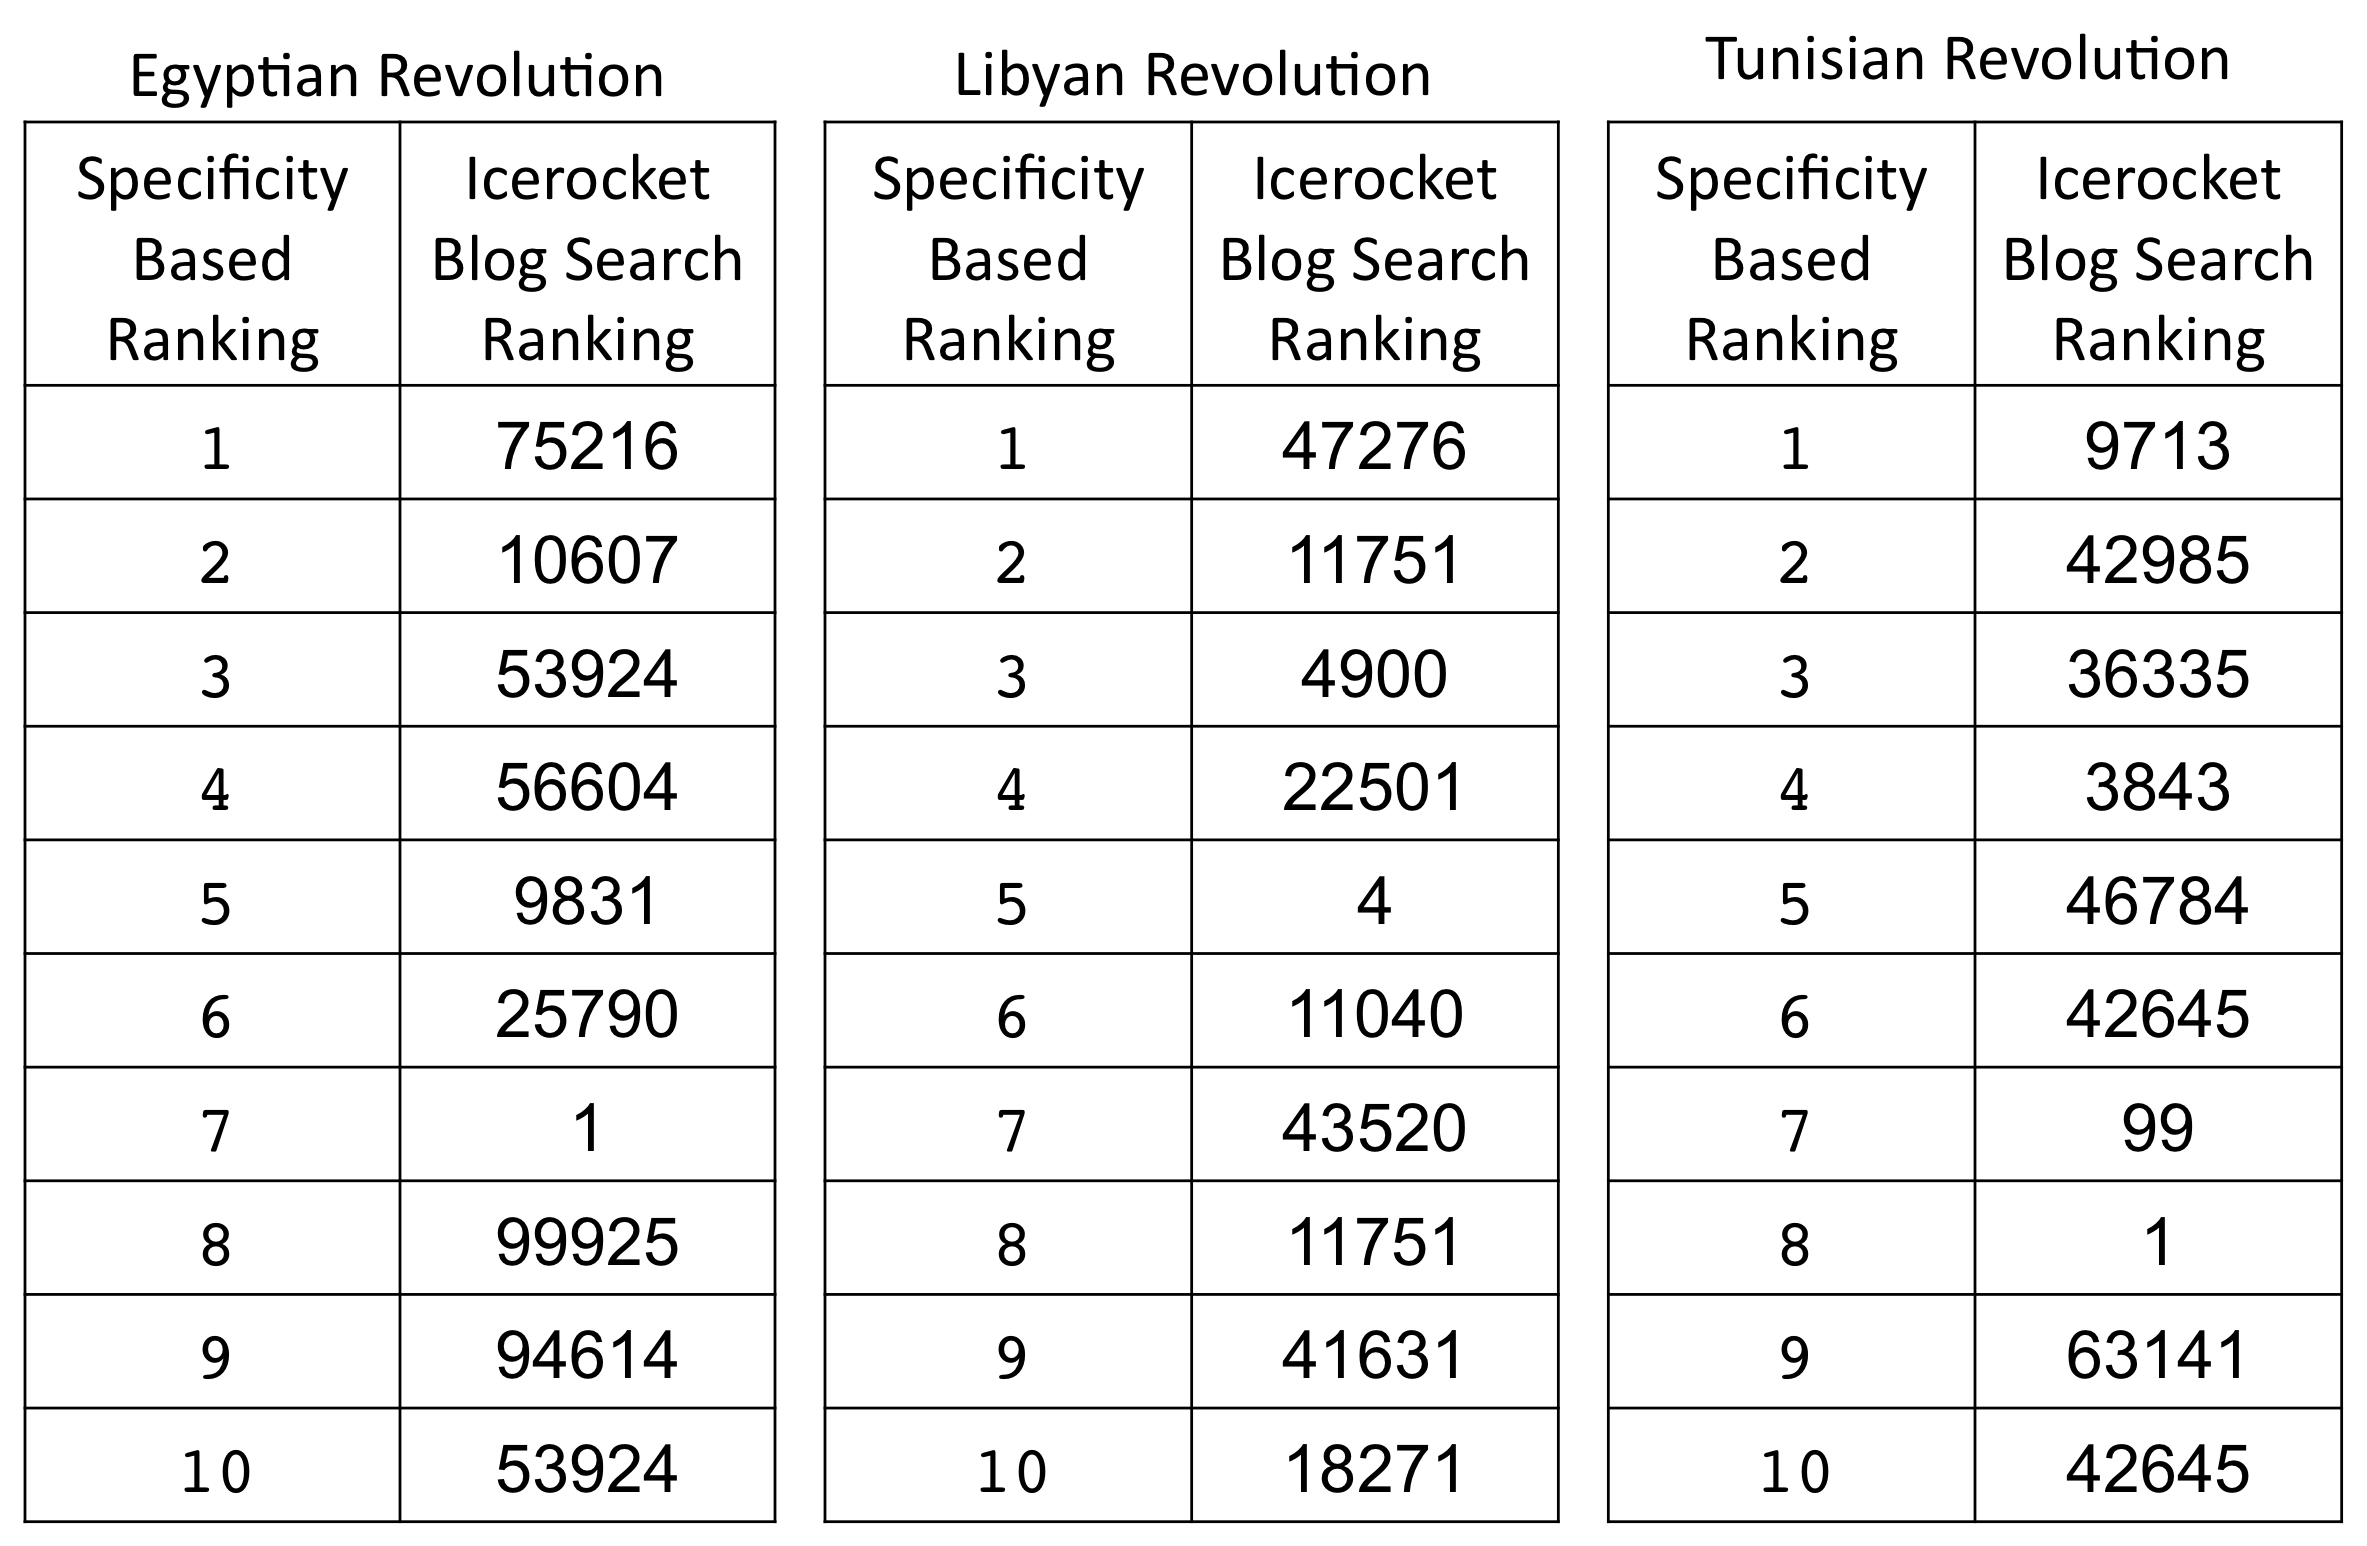
\includegraphics[height=2in,width=3.5in]{Figures/Chapter3Figures/RankDistIceRocket.jpg} 

\end{array}$
\caption{Rankings of the sources from Google Blogger and Icerocket based on `specificity' $(\kappa)$ values obtained from our model and the rankings assigned by Google Search and Icerocket Blog Search.}
\label{fg:figure22}
\end{figure*}

\begin{figure*}[htbp]
\centering$
\begin{array}{cc}
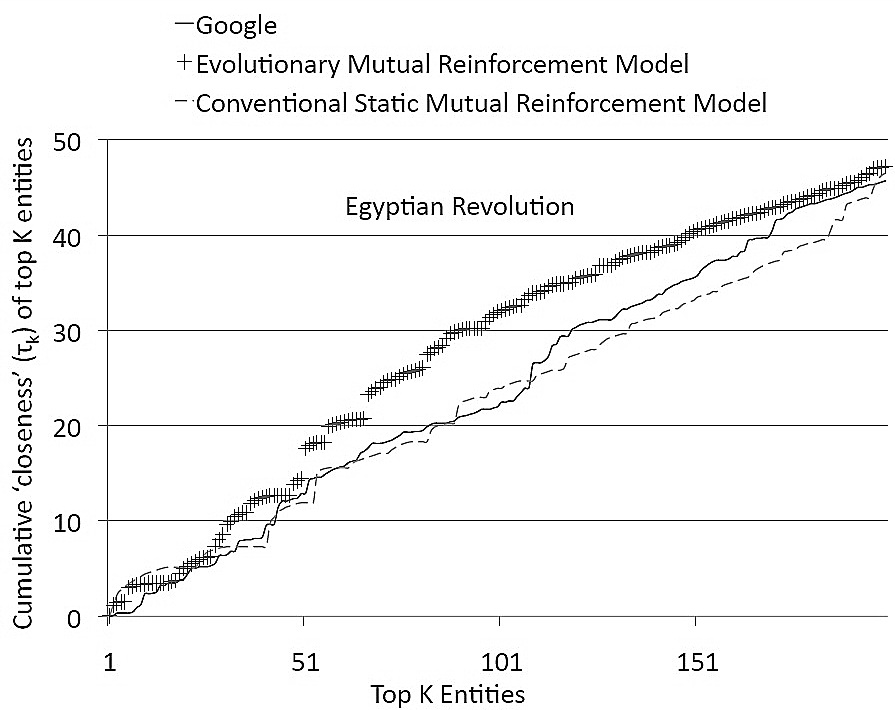
\includegraphics[height=2.3in,width=2.3in]{Figures/Chapter3Figures/GrayedImages/googleEgyptCumulative.jpg} &
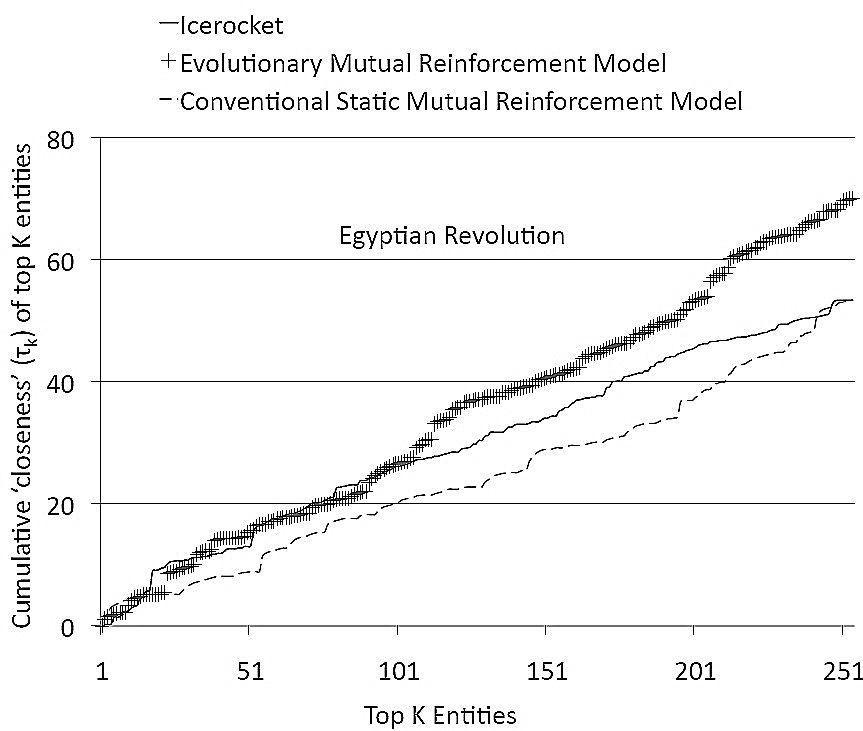
\includegraphics[height=2.3in,width=2.5in]{Figures/Chapter3Figures/GrayedImages/icerocketEgyptCumulative.jpg} \\
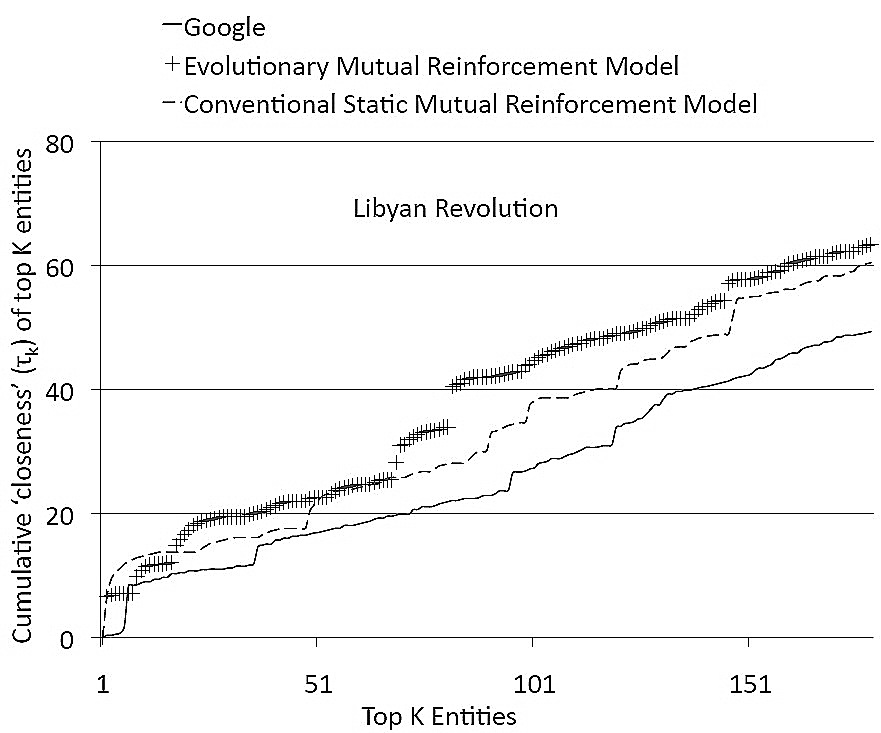
\includegraphics[height=2.3in,width=2.3in]{Figures/Chapter3Figures/GrayedImages/googleLibyaCumulative.jpg} &
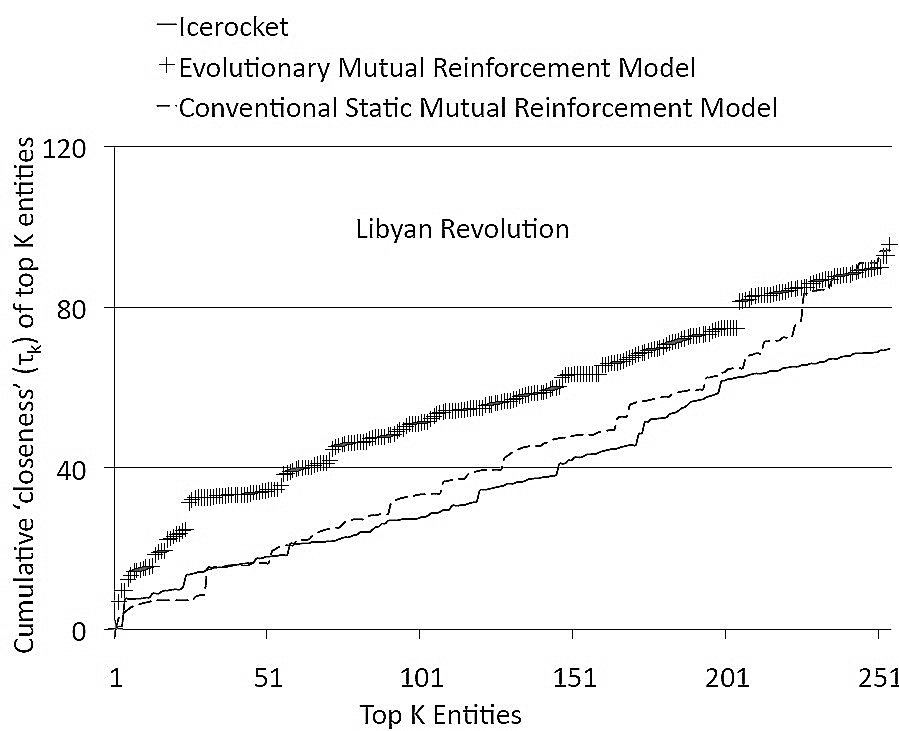
\includegraphics[height=2.3in,width=2.3in]{Figures/Chapter3Figures/GrayedImages/icerocketLibyaCumulative.jpg} \\
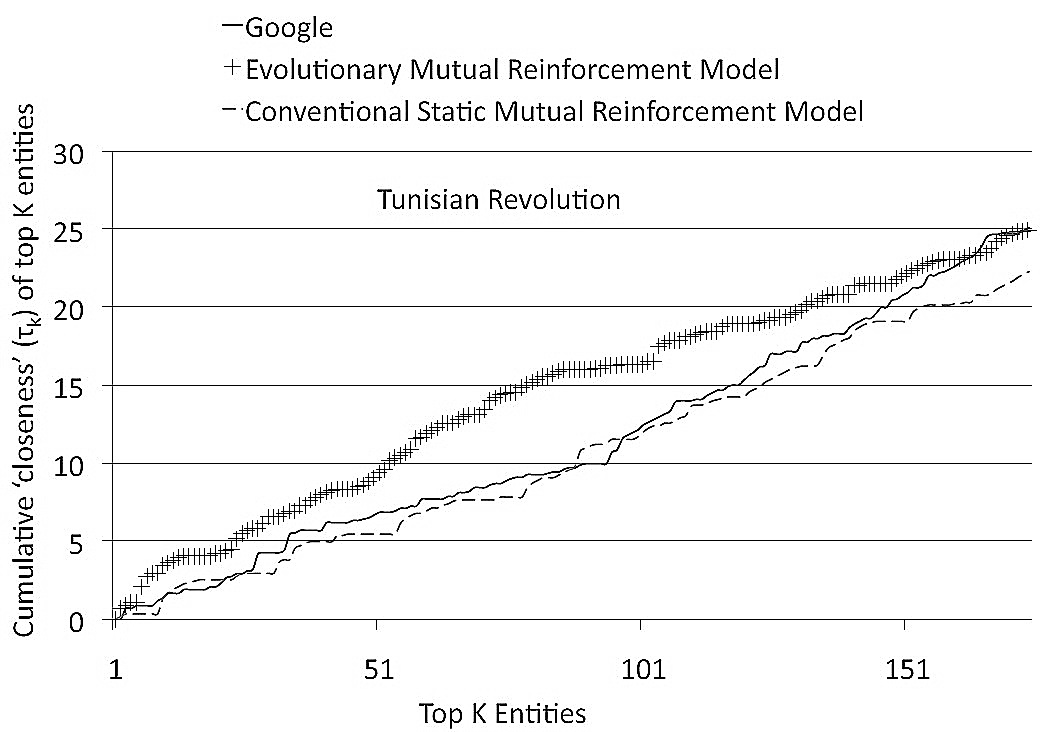
\includegraphics[height=2.3in,width=2.3in]{Figures/Chapter3Figures/GrayedImages/googleTunisiaCumulative.jpg} &
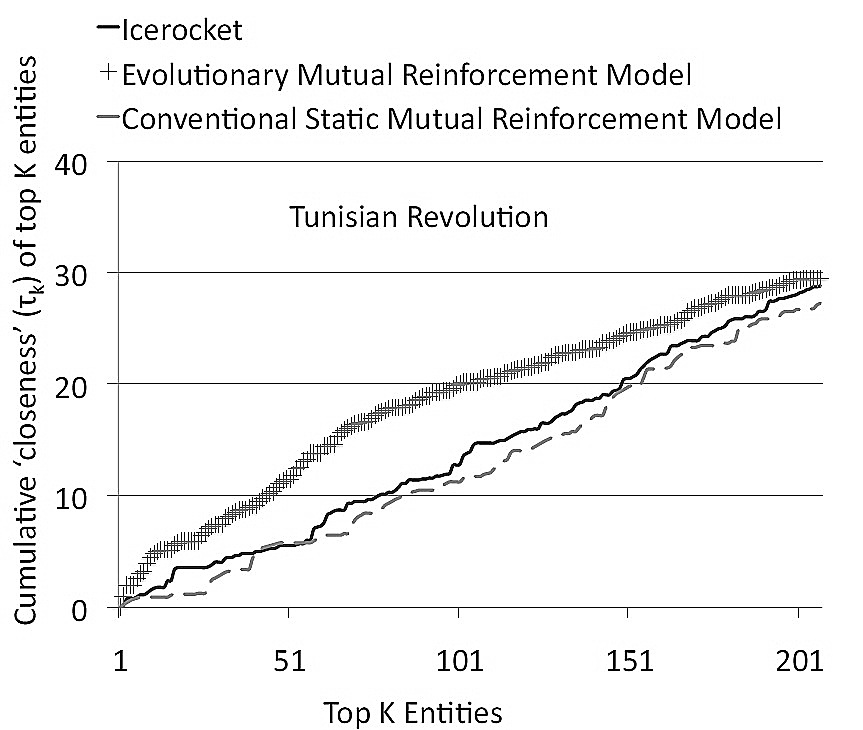
\includegraphics[height=2.3in,width=2.3in]{Figures/Chapter3Figures/GrayedImages/icerocketTunisiaCumulatice.jpg}
\end{array}$

\caption{Validating specific sources obtained from our model.}
\label{fg:figure3}
\end{figure*}






\subsection{\label{basecomp}\textbf{Baseline Comparisons}}

\noindent \textit{\textbf{Selecting the Baselines:}} Due to lack of benchmark datasets we use the search results obtained from Google and Icerocket Blog Search as baselines for validation. Standard information retrieval measures for evaluation (DCG, NDCG, MAP, MAP@10) could not be used due to the absence of ground truth. We also consider the sources ranked according to the conventional static mutual reinforcement model and show the effectiveness of our model in quickly gaining information about an event. We further analyze the ranking of the top K specific sources as identified by our methodology and observe the difference in their rankings as assigned by the search engines and as assigned by our model. Figure \ref{fg:figure22} shows ranks assigned by Google and Icerocket for the top 10 sources for each event, ranked according to our framework. We conclude, that  our framework could identify the sources that often gets buried in the Long Tail and has the potential for presenting valuable information about the event. Next, we propose a novel strategy to demonstrate the effectiveness of the specific sources ranked by our evolutionary mutual reinforcement model in identifying highly informative sources.


\noindent \textit{\textbf{Rationale Behind The Strategy:}} Search engines are designed to give the most relevant sources containing the close entities, related to a query for a given event. As these close entities have a very high probability to be associated with the event, we expect to gain valuable information about the event from these entities making the highly ranked sources very specific to the event. We use this notion to propose a novel evaluation strategy, showing that when sources related to an event are ranked according to our model, they provide more valuable information than the ranking order given by the search engines and the conventional mutual reinforcement model for the same set of sources.


\noindent \textit{\textbf{Implementation of The Strategy:}} We compare closeness ($\tau(e_{i})_{E_{j}}$) values of the entities obtained from the sources ranked according to the search engines, the conventional model  and our model respectively. Following steps are taken,
\begin{itemize}

\item \noindent \textit{\textbf{Preparing the Ranked Lists of Entities:}} From the three differently ranked lists (search engine, our evolutionary model and conventional static model), each source is visited and the entities are extracted from them. The `$\tau(e_{i})_{E_{j}}$' values are assigned to these entities by referring to the respective final event dictionary ($\varsigma_{E_{j}}$) and they are ranked in descending order. 

\item \noindent \textit{\textbf{Measuring the Information Gain:}} As we traverse the three list of sources, we obtain three list of same entities, arranged in different orders depending upon the ranking of the sources. In order to show the comparison  in the gain of information from the three lists we take the top `K' entities from each list and calculate the sum of their `$\tau(e_{i})_{E_{j}}$' values and plot them against the value of `K' in Figure \ref{fg:figure3}. We start from K=1 and go on increasing its value till the number of entities are exhausted in all the three lists. It is evident from Figures \ref{fg:figure3}, that the curves based on specificity ($\kappa(S_{i})_{E_{j}})$ quickly gains over the curves based on the search engines and the conventional model. 

%\vspace{-3pt}
\item \noindent \textit{\textbf{Analysis:}} Figure \ref{fg:figure3} shows that information about the event is gained quicker using our model, which could identify specific sources earlier than the search engines as well as the conventional model. We measure the maximum percentage gain of information in each set of sources related to the three events. There is a maximum gain of information (130.4\%) in case of sources obtained from Icerocket search related to `Tunisian Revolution', and a minimum gain of information (25.97\%) in case of the sources obtained from Icerocket search related to `Egyptian Revolution'. Also when the sources are ranked according to our methodology they gain the maximum percentage of information at the $9^{th}$ source in case of sources obtained from Google related to `Libyan Revolution'. This in turn implies that the sources ranked higher by our model are more specific than the ones ranked by the search engines and the conventional model. These highly specific sources are also very informative. When presented earlier they also help in learning useful information about the event due to the presence of close entities in them. As we already observed earlier that these sources are often Long Tail sources, we can conclude that Long Tail sources that are ranked lower by the search engines, when identified are often more specific than the highly ranked short head sources. 

\end{itemize}



%Apart from giving better results, our evolutionary model also showed faster convergence than the conventional static mutual reinforcement model. The number of iterations taken by the power iteration method to converge in each case is analyzed in Figure \ref{fg:figure12}. It is observed that the number of iterations taken by the power iteration method is lesser, whenever we employ our evolutionary mutual reinforcement model. 
\begin{table*}[htbp]

\caption{\small Top 5 entities in the event specific and the event class dictionaries constructed for the set of events $\xi$.}
\label{tab:table2}
\centering
\begin{tabular}{|l|p{5cm}|}
\hline
\textbf{Egyptian Revolution Specific Dictionary} & Tahrir Square, Egyptian government, Gigi Ibrahim, Alexandria, Wael Abbas. \\
\hline
\textbf{Libyan Revolution Specific Dictionary} & Tripoli, Muammar Al Gaddafi, North Atlantic Treaty Organization, Chad, United Kingdom \\ 
\hline
\textbf{Tunisian Revolution Specific Dictionary} & Tunisian government, Lin Ben Mhenni, Samir Feriani, Kasbah Square, RCD \\ 
\hline
\textbf{Socio-Political event dictionary} & Twitter, Iranian Government, Tear gas devices, Facebook, Big Social network \\ 
\hline
\end{tabular}
\end{table*}
\vspace{-3pt}

\section{\label{explore}\textbf{Further Exploration}}

\begin{figure}[htbp]
\centering$
\begin{array}{c}
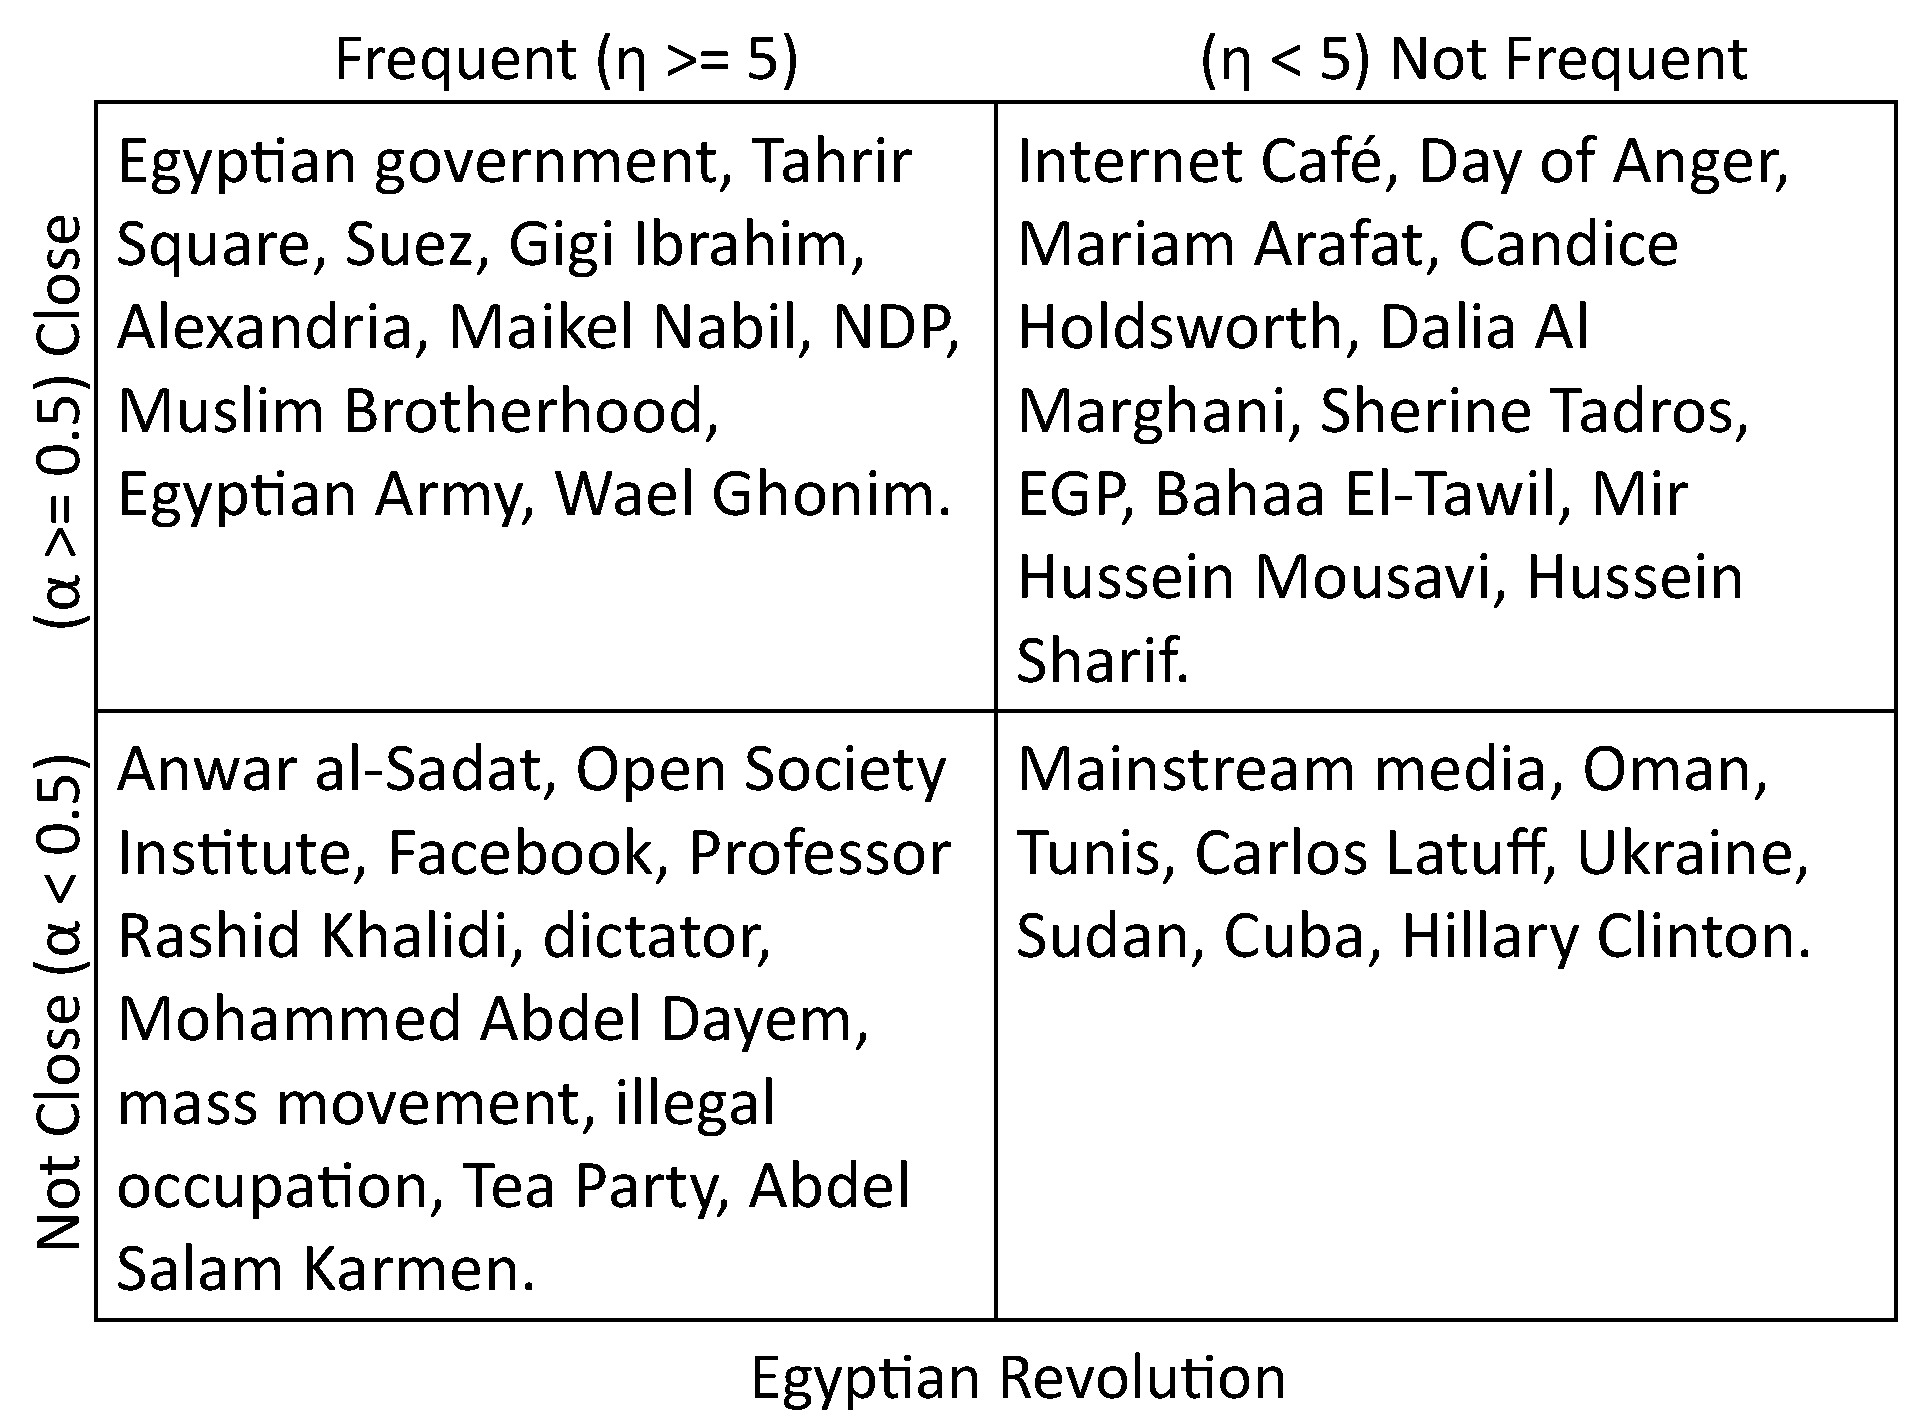
\includegraphics[height=3in,width=4in]{Figures/Chapter3Figures/confusionMatrixEgypt.pdf} \\
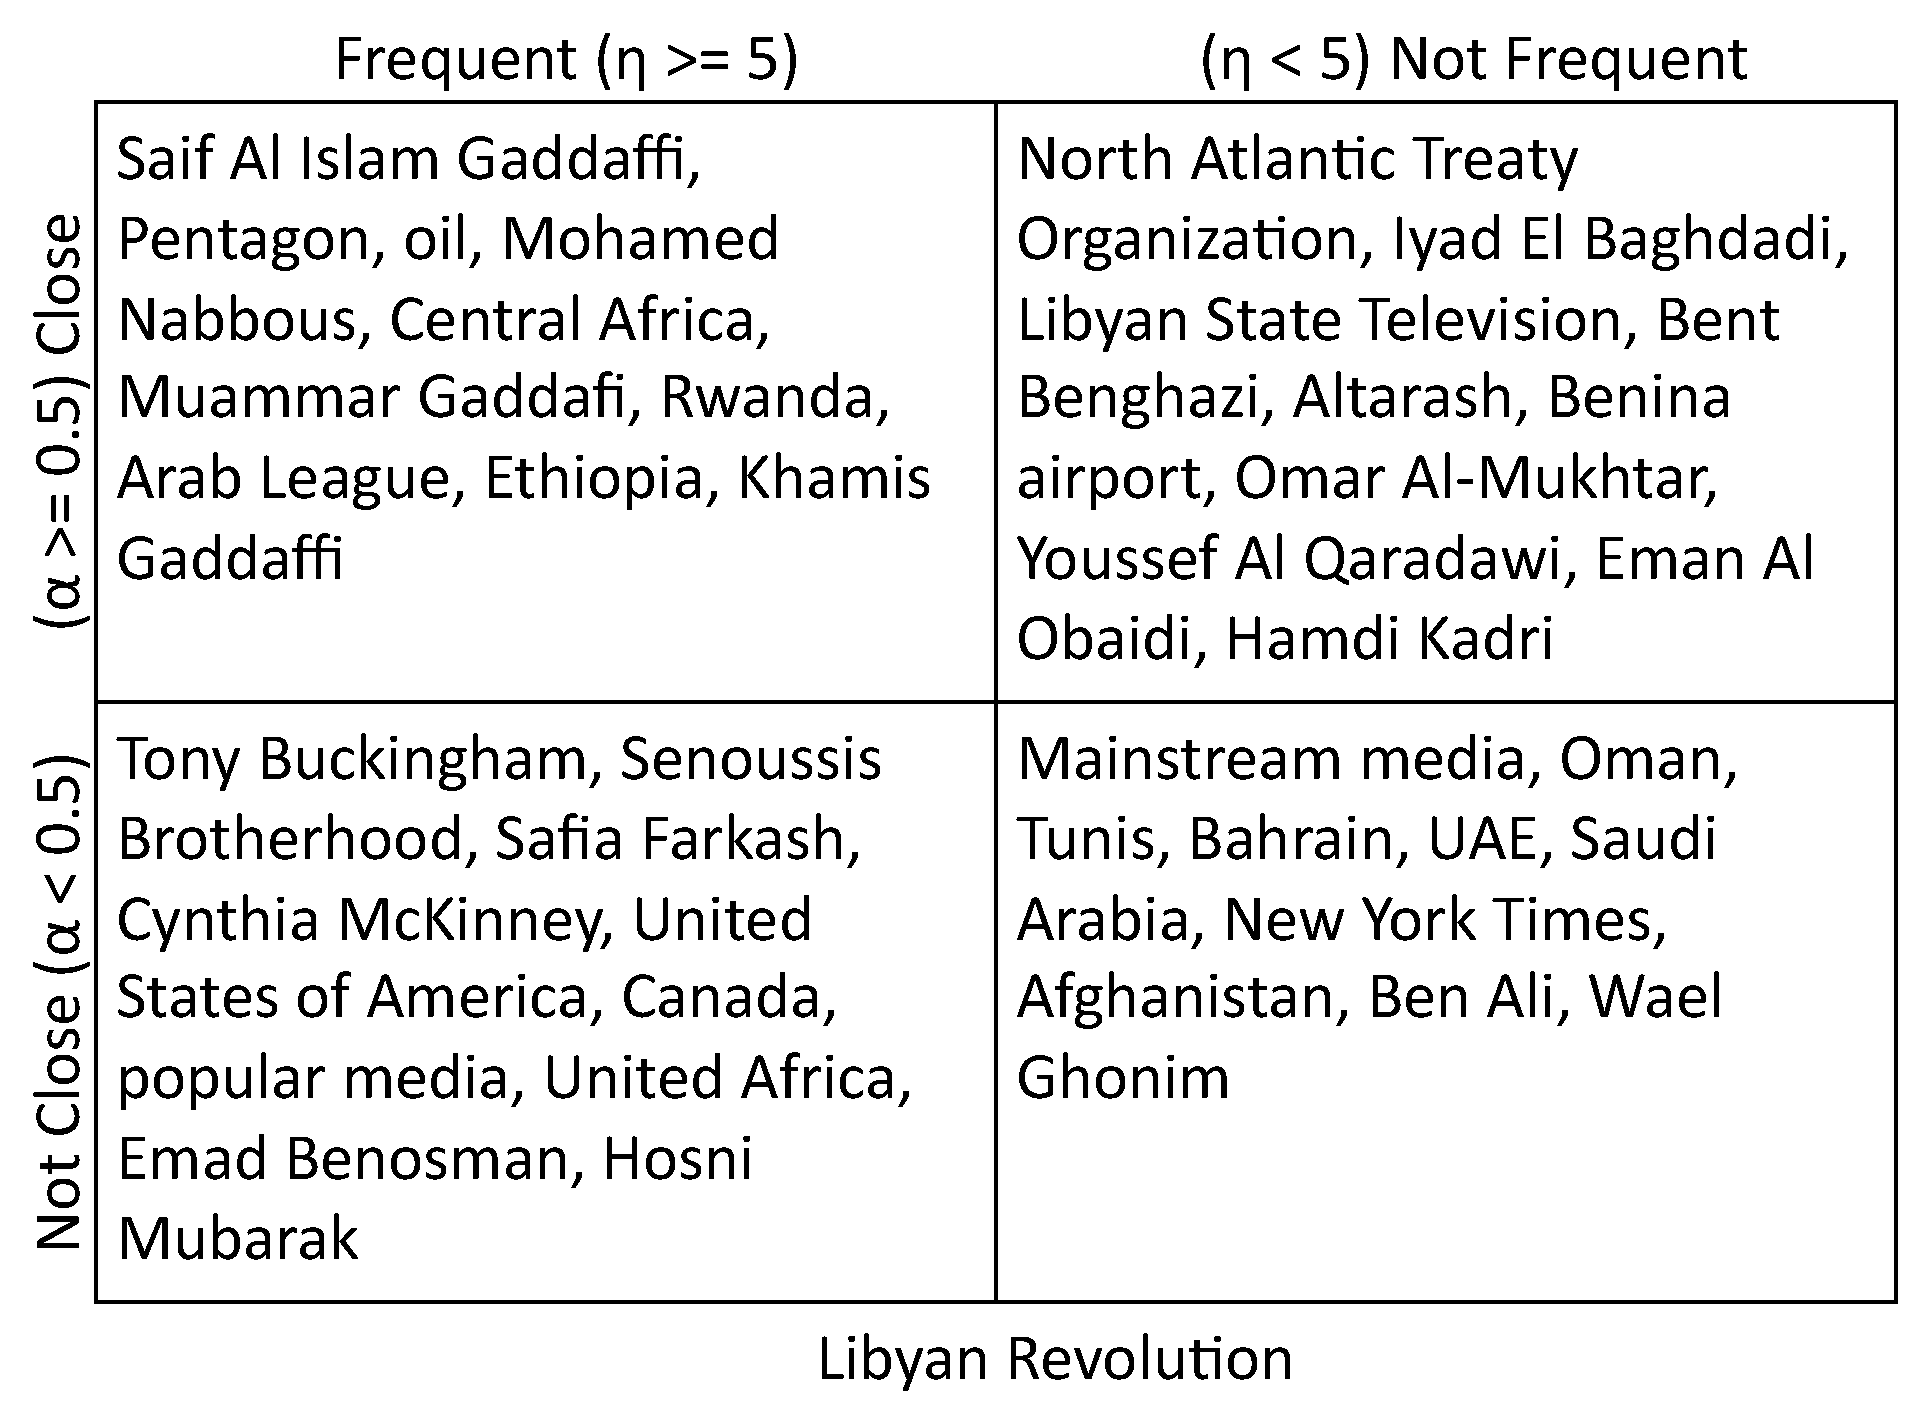
\includegraphics[height=3in,width=4in]{Figures/Chapter3Figures/confusionMatrixLibya.pdf} \\
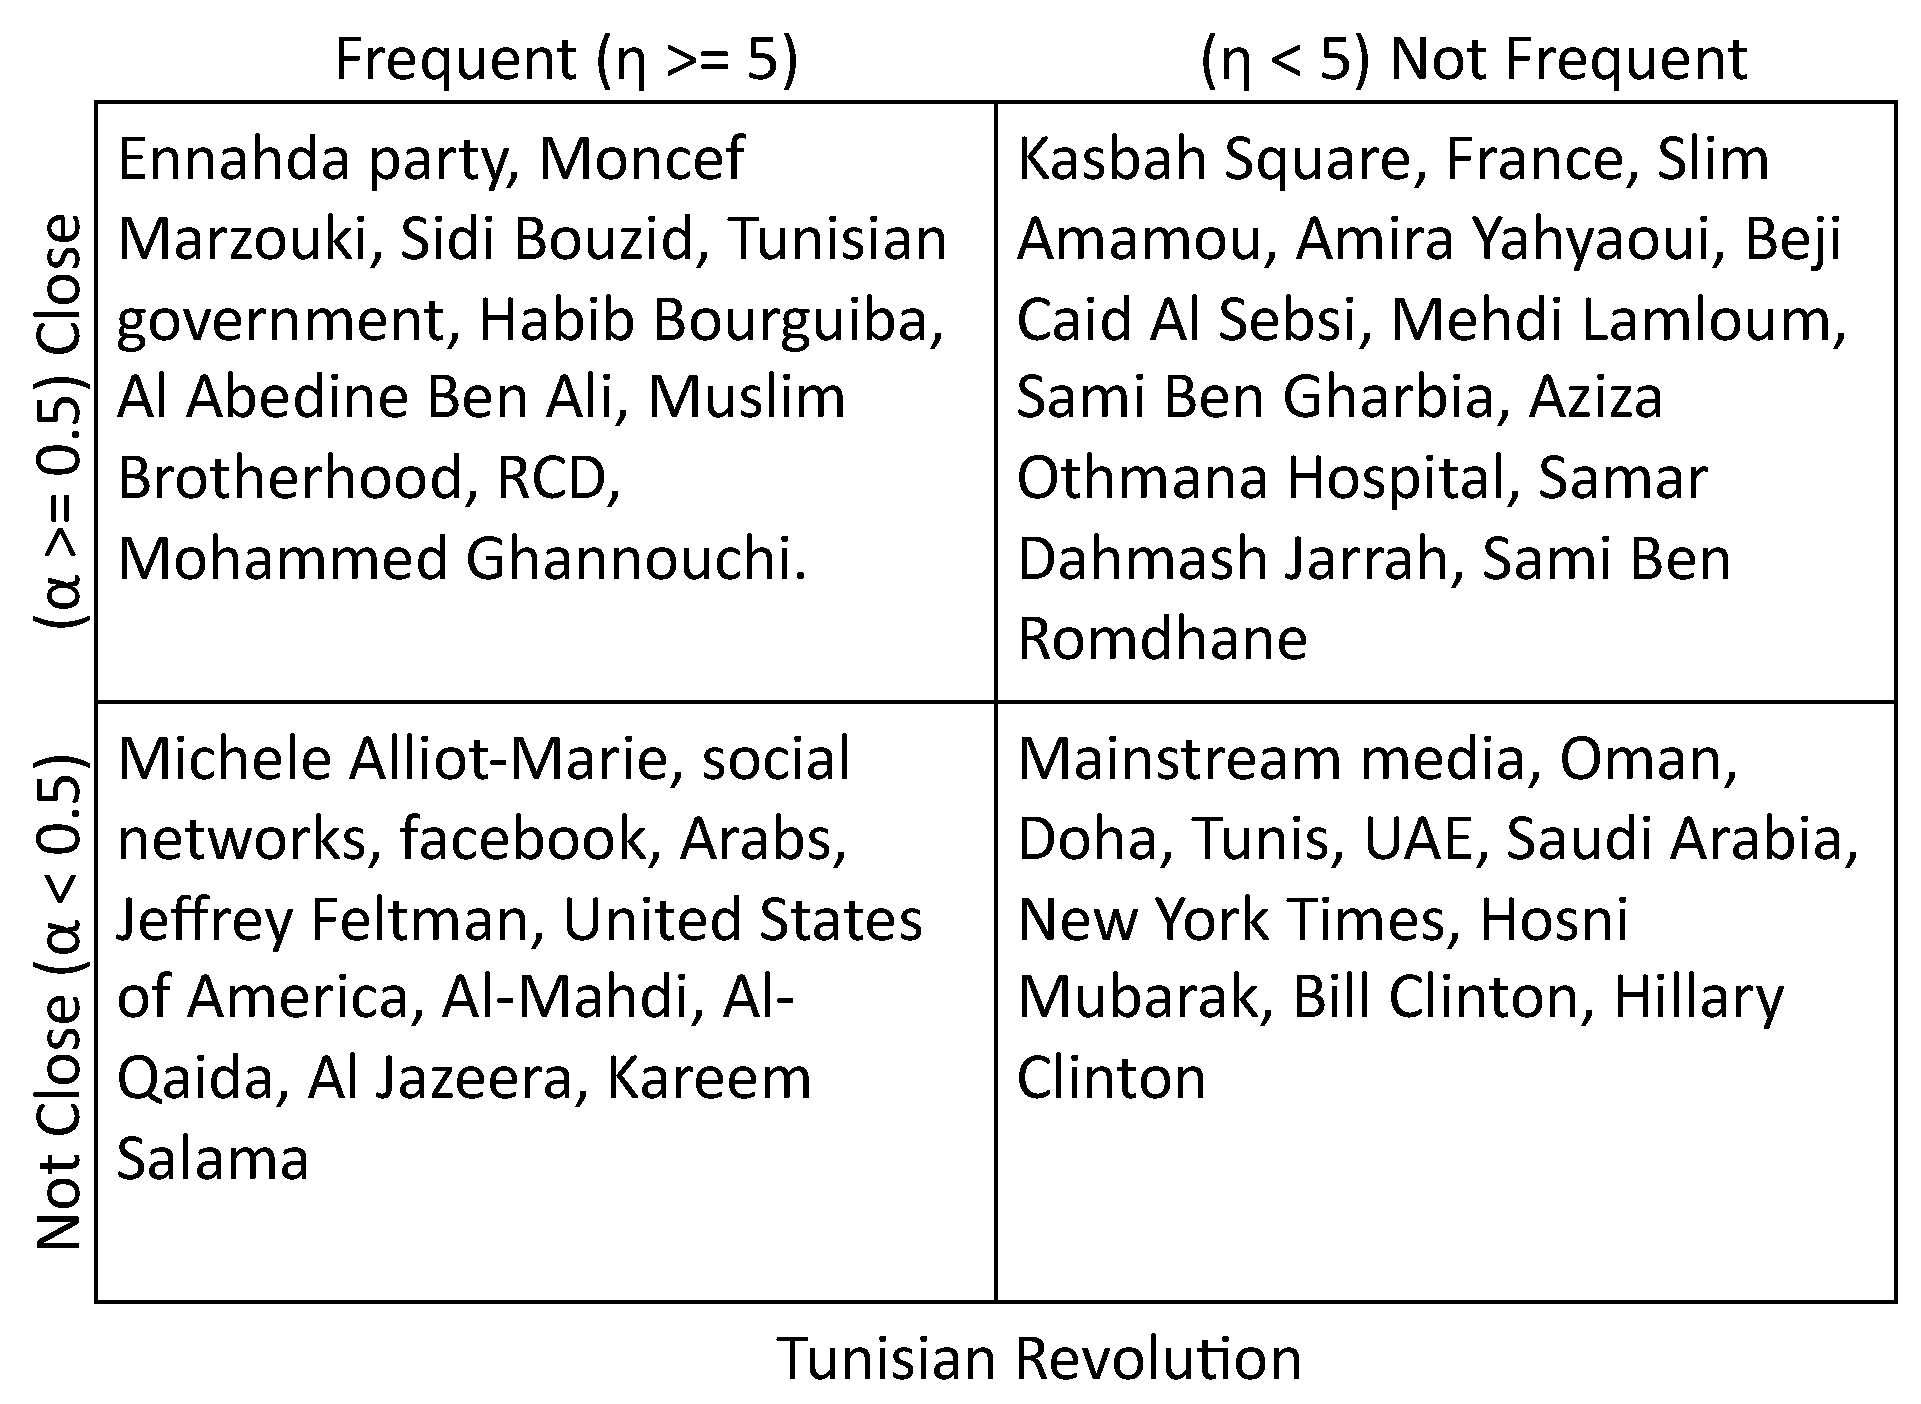
\includegraphics[height=3in,width=4in]{Figures/Chapter3Figures/confusionMatrixTunisia.pdf}


\end{array}$

\caption{Different categories of entities for the events.}
\label{fg:figure5}
\end{figure}

%The proposed model helps in identifying closer entities and specific sources related to an event. 

We use the proposed framework developed by us as an apparatus to further explore event characteristics and show its utility in analyzing events. We show the potential of the final event dictionaries ($\varsigma_{E_{j}}$) obtained for each event $E_{j}$ for gaining valuable information about the event and to identify the generic entities related to the class of events. 

The entities in the final event dictionaries ($\varsigma_{E_{j}}$) are examined further. Based on their frequency $f(e_{i},E_{j})$ and closeness $(\tau(e_{i})_{E_{j}})$ scores, we categorize the entities into the following categories: a. \textit{Close and Frequent}, b. \textit{Close but Not Frequent}, c. \textit{Not Close but Frequent}, and d. \textit{Neither Close nor Frequent} as shown in Figure 7. We categorize an entity in each event dictionary as `frequent' if it occurs more than a threshold value $\eta$ i.e $f(e_{i},E_{j}) \ge \eta$, and `close' if it has   a closeness score more than a threshold value $\alpha$ i.e $\alpha \ge \tau(e_{i},E_{j})$. After careful manual inspection we decided the values of $\eta$ and $\alpha$ to be 5 and 0.5 respectively. The values of $\eta$ and $\alpha$ is same for all the events $E_{j} \in \xi$. However, different thresholds could be examined in the future though. Each entry in a matrix, consists of top 10 entities that satisfy the thresholds for the corresponding row and column category. We further examine  these entities in the context of each of these events and report interesting observations. We present the observations for ``Egyptian Revolution'', next, however similar observations were made for other events.



%The classification of entities helped us to analyze the event dictionaries from different perspectives as explained in the following subsections.
\subsection{\textbf{Event-specific Popular and Close Entities}}
We analyze the entities in the \textit{Close and Frequent}, and \textit{Close but Not Frequent} categories. We find that \textit{Close and Frequent} entities are not only frequent but are also closely related to the event. In other words these are very popular entities related to the event. For example, the occurrence of `Tahrir Square' and `Egyptian government' in this category, is inevitable, as Tahrir Square is the place where the protest started against the Egyptian Government. These are also the entities that anyone comes to know about from the top search results given by the search engines as well as from mainstream media sources. 

%So we further classify them as \textit{event-specific popular} entities. 

On the other hand, \textit{Close but Not Frequent} category primarily consists of entities that add novel and useful insights to the events. The occurrence of `Internet Cafe' in this category clearly shows how the local people in Egypt used Internet Cafes for accessing various social media websites in order to coordinate and participate in the revolution. It is also the place where `Khaled Said', a 28 year old computer-wiz was arrested by the Egyptian police. He was brutally tortured to death, triggering the anger among the people of Egypt for a mass uprising against the dictatorial government.  January 25, 2011 is also known as `The Day of Anger' in the Egyptian Revolution, as it is the day that marked the start of a series of protests and riots in Egypt. So the occurrence of the entity, `Day of Anger' in this category is reasonable. 

%So we further classify them as \textit{event-specific local} entities. 

Drawing upon the differences between the two categories our findings suggests that although the category of \textit{Close and Frequent} entities give a lot of information about an event, it is also necessary to know about the entities of \textit{Close but Not Frequent} category. The entities belonging to \textit{Close but Not Frequent} category provides in-depth information about the event from the grass root level. The \textit{Close but Not Frequent} entities are likely to be found buried in the Long Tail sources. In order to gain maximum information about an event it is necessary to identify the entities from both the categories. They point to the key persons, places and organizations related to the event. In other words, these entities when present in a source makes it highly specific to the event. Both these categories of entities can prove to be vital sources of information about the event. 



\subsection{\textbf{Event-specific and Event-class specific dictionaries}}
Based on the categorization and the analysis conducted in the previous subsection we divide the final event dictionaries ($\varsigma_{E_{j}}$) for each event into \textit{event-specific} and \textit{event-class specific} dictionaries. The \textit{event-specific} dictionaries are comprised of the entities categorized as \textit{Close and Frequent}, and \textit{Close but Not Frequent} for each event $E_{j} \in \xi$ respectively. Whereas, the \textit{event-class specific} dictionary is comprised of the entities found in the \textit{Not Close but Frequent} and \textit{Neither Close nor Frequent} categories for all the events $E_{j} \in \xi$.

Table \ref{tab:table2} shows the top five entities in the \textit{event specific} dictionaries for each event $E_{j}$ and a socio-political event dictionary for the set of events $\xi$ under study. The entities in the \textit{event specific} dictionaries, when present in a source makes it highly specific to that particular event and contributes in gaining information about it. These entities can also help in conducting micro-analysis of an event by identifying precise details about the event. On the other hand, the entities of the \textit{event-class specific} dictionary provides shallow information about a specific event, and are useful in learning about a category of events, in this case, socio-political uprisings in the middle east. These entities can help in conducting macro-analysis of an event by classifying the event into a certain category (like socio-political, crisis, entertainment, economic, etc.) and point out the general characteristics of the event. However, the analysis requires a set of known events, which could be a perceiveable constraint. We plan to address this in the future work. 

%Next, we present the related work and compare and contrast  these with the proposed approach, highlighting our contributions to the literature.

%Thus we conclude that, the first two categories of entities are very helpful in conducting a micro analysis and in knowing precise details about the events. When present in a source they make it highly ‘specific’. The other two categories are helpful for macro analysis. Although they provide shallow information about a specific event, they are useful in learning about a category of events, in this case, socio-political uprisings.



%\subsection{Analyzing the dictionary}



%The event dictionaries finally obtained enable us to further conduct micro (related to very specific) and macro (related to generic) analysis of the events. The entities in the event dictionaries are examined further. Based on their frequency and closeness $(\tau(e_{i})_{E_{j}})$ values, we create confusion matrices of entities for each of the events as shown in Figure 9., categorizing the entities into the following categories: a. Close and Frequent, b. Close but Not Frequent, c. Not Close but Frequent, and d. Neither Close nor Frequent. After studying the frequency distribution and `$\tau$' values of the entities in the event dictionaries we decided to classify an entity as `frequent' if it occurs more than five times for the set of sources for that event and `close' if it has a value greater than equal to 0.5 for `$\tau$'.  Each entry in a matrix, consists of top 10 entities that satisfy the conditions for the corresponding row and column category. We further examine  these entities in the context of each of these events and make some interesting observations. We present the observations for ``Egyptian Revolution'', next, however similar observations could be made for other events.

%\begin{itemize}
%\item `\textit{Close and Frequent}' entities are not only popular but are also closely related to the event. For example, the occurrence of `Tahrir Square' and `Egyptian government' in this category, is inevitable, as Tahrir Square is the place where the protest started against the Egyptian Government. 
%
%%\item `\textit{Close but Not Frequent}' category primarily consists of `local' entities. These entities add useful insights to the events. The occurrence of `Internet Cafe' in this category clearly shows how the local people in Egypt used Internet Cafes for accessing various social media websites in order to coordinate and participate the revolution. It is also the place where Khaled Said, a 28 year old computer-wiz was arrested by the Egyptian police. He was brutally tortured to death, triggering the anger among the people of Egypt for a mass uprising against the dictatorial government.  January 25, 2011 is also known as `The Day of Anger' in the Egyptian Revolution, as it is the day that marked the start of a series of protests and riots in Egypt. So the occurrence of the entity, `Day of Anger' in this category is reasonable.
%
%\item `\textit{Not Close but Frequent}' and `\textit{Neither Close nor Frequent}' entities do not contribute much in gaining `specific' information about the events. Entities like `Facebook', `United States of America' , `New York Times', etc are popular in their own rights. They may not be important in the context of the indiividual events and provides very generic information about the set of events under analysis.
%
%\end{itemize} 
%Thus we conclude that, the first two categories of entities are very helpful in conducting a micro analysis and in knowing precise details about the events. When present in a source they make it highly ‘specific’. The other two categories are helpful for macro analysis. Although they provide shallow information about a specific event, they are useful in learning about a category of events, in this case, socio-political uprisings.

 



\section{\label{future}\textbf{Conclusions And Future Work}}

In this paper, we highlighted the need for exploring the social media sources to study an event that are often buried in the Long Tail. We demonstrated that social media sources have the capability to provide very specific and novel information. However, the sheer volume of social media sources and the Long Tail characteristics (e.g., link sparsity, colloquial language, etc.) make it extremely challenging to identify the specific sources. Towards this direction, we developed a methodology that utilizes relevant entities as a mechanism to identify specific sources in a mutual reinforcement framework. Further, in order to consider the dynamic relationship between the specific sources and close entities, an evolutionary mutual reinforcement model is developed. Experiments conducted on real-world datasets for the three social movements during the Arab Spring, viz., Egyptian Revolution, Libyan Revolution, and Tunisian Revolution demonstrate faster convergence and better accuracy of the evolutionary mutual reinforcement model over the conventional mutual reinforcement model. Furthermore, the evolutionary mutual reinforcement model outperformed one of the most-widely used search
engines, i.e., Google Blog Search and IceRocket. It was observed that the search engines ranked the specific sources surprisingly low, thereby reducing the chances of their discovery. The poor hyperlink connectivity of these Long Tail social media sources was contemplated to be a big reason behind their low ranks in traditional search engines. By analyzing the close entities identified by our model we also showed the potential of the framework to be utilized for analyzing events. In future, we plan to explore the proposed framework in assessing credibility of the Long Tail social media sources, which are known to disseminate false reports for breaking events. We also plan to use the framework in order to identify users with sustained interest in different events.
 
%% Chapter 5

\chapter{Discovering Event-specific Informative Content from Twitter} % Main chapter title

\label{TwitterStudy} % For referencing the chapter elsewhere, use \ref{Chapter1} 

\lhead{Chapter 5. \emph{Discovering Event-specific Informative Content from Twitter}} % This is for the header on each page - perhaps a shortened title

\section{Twitter and Event Related Content}

\section{Analysis of Informative and Non-informative Content in Tweets}

\section{EventIdentityInfoGraph}

\section{EventIdentityInfoRank}

\section{Experiments}

\subsection{Data Collection}

\subsection{Data Preparation}

\subsection{Baselines}

\subsection{Evaluation}

\subsection{Sample Results} 
%% Chapter 6

\chapter{Potential Applications of the EIIM Framework} % Main chapter title

\label{applications} % For referencing the chapter elsewhere, use \ref{Chapter1} 

\lhead{Chapter 6. \emph{Potential Applications of the EIIM Framework}} % This is for the header on each page - perhaps a shortened title

\section{Event Monitoring and Analysis}
References related to real-life events are extremely abundant in social media. Right from natural disasters such as the `Haiti Earthquake' \cite{gao2011harnessing} to international sporting events like the `Winter Olympics' \cite{walker2013russia} to socio-political \cite{singh2010mining} and socio-economical \cite{bollen2009modeling} events that shook the world such as presidential elections \cite{metzgar2009social}, `Egyptian Revolution' \cite{choudhary2012social}, and recessions were covered, analyzed, extrapolated and informed by social media. This prolific event-specific content in social media makes it a promising ground for performing event analytics. Platforms like Geofeedia\footnote{http://geofeedia.com/}, TwitterStand\footnote{http://twitterstand.umiacs.umd.edu/}, Twitris\footnote{http://twitris.knoesis.org/}, Truthy\footnote{http://truthy.indiana.edu/}, and TweetTracker\footnote{http://tweettracker.fulton.asu.edu/}  have developed techniques to provide analytics related to different local and global real-life events. 

Monitoring social media has become one of the essential activities of national security agencies for predicting potential threats and mass protests \cite{ghannam2011social}. Social media is being used for tracking terrorism activities \cite{oh2011information}, collective actions \cite{agarwal2014online}, and countering cyber-attack threats\footnote{https://www.recordedfuture.com/}. One of the main components of each of these applications is tracking references related to the events. The proposed EIIM model could be an essential component of such systems. It would help in identifying, tracking and analyzing events and its related references in an organized manner over time.



\section{Event Information Retrieval}
Retrieving informative content related to real-life events shared in social media and presenting them in an organized way to the interested users has led to web based services like Seen\footnote{http://seen.co}. It allows users to follow live updates of the events and also aids in witnessing and re-living the events at a later stage from the archives. Showing useful and interesting content to users by filtering out the pointless babbles from social media streams is an important component of such services. Additionally, such systems could get immensely benifitted by identification of event-specific informative hashtags, text units, users and URLs over time as the event proceeds. This would further enable efficient indexing of event-specific terms and hashtags that leads to high quality information, and effective processing of information. It would enhance the user experience, allowing better consumption and summarization of information related to the events, and positively impact triggering of event-specific recommendations. Thus, the proposed EIIM model in this thesis can act as the core component of information retrieval systems retrieving and organizing information related to real-life events from social media. 

\section{Opinion and Review Mining}
Every day millions of people express their opinions in social media about products and companies they like and dislike. Their communications often include thoughts about good and bad experiences with the products and services. This provides a great opportunity for companies to understand its customers and to get unbiased valuable feedback from them about their product offerings without asking them to fill out time consuming outdated surveys. The EIIM framework when used for monitoring references of products/services from social media during product launch events could be useful in mining isightful and informative opinionated content. Combined with sentiment analysis, the invention could be a powerful tool for review analysis. One of the important contributions of the system could be to identify the sources having high chances of containing insightful information and filter them out for further processing. This would make a review mining system more efficient and increase its overall quality. Mining opinions related to entities related to an event could be used in many other contexts like political campaigns, socio-political studies, market behavior analysis, e-commerce applications, etc. Steps are being taken for adding this capability to the EIIM framework. On considering a mix of named entities and unigram opinionated words as text units in the \textit{EventIdentityInfoGraph} we obtained some preliminary encouraging results. A glimpse of the results obtained for a basketball game ''Miami Heats VS Cleveland Cavaliers", played on 25th December, 2014 is as follows:

Top 10 insightful and opinionated tweets for an hour related to the game
\begin{enumerate}

\item	Good win for the Heat tonight against Cavs and Lebron. Great game for Wade and Deng. Just imagine if Bosh were healthy. \#HeatvsCavs

\item	Good work Dwayne Wade. Good work Miami Heat. LeBron is embarrassed. It's all over his face. \#NBA \#heatvscavs

\item	Great game on Christmas Heat Showed up and spoiled Lebron Return to MIA! \#Wade County \#HeatvsCavs \#NBAChristmas

\item	Lebron leaves Miami high and dry and they cheer his return. Some even cheering cavs. Embarrassing bandwagon fan base. \#heatv…

\item	I totally understand LBJ move to Cleveland and like it. But if I'm a \#Miami fan, I would boo LeBron like crazy today. \#heatvscavs \#CLEvsMIA

\item	Stay classy \#Miami. Good game vs. Lebron and; Cavs. \#NBA \#MIAvsCLE \#HeatvsCavs \#Heat \#HeatNation

\item Loul Deng playing both ends of the floor. He's playing good D to LBJ \#heatvscavs

\item	Heat fans ; Cavs fans. Class vs no class. No burning a jersey in Miami \#heatvscavs \#HeatNation

\item	WE FUCKING WON!!!!!! LETS GO HEAT \#HEATgame \#HeatNation \#HeatvsCavs Wade with 31 points 5 assist 5 rebounds! Good shit MIAMI

\item	Kevin Love is overrated. Big fish, small pond in MN and injury prone. \#HeatvsCavs \#NBAXmas

\end{enumerate}

The above tweets point to the reactions of the viewers on the game as well as the players participating in the event.

\section{Recommender Systems}
The EIIM framework can be used for developing event related recommender systems. The ranked list of event identity information can be used for giving useful recommendations. For example following is a refined tweet recommendation for an event obtained from a snapshot of the \textit{EventIdentityInfoGraph} created for the event: “BlackLivesMatter”: Protest movement against the killing of Eric Garner.

\textbf{Original Tweet:}

\begin{itemize}
\item \#BREAKING \#NEWS | New York City Mayor Says, \#BlackLivesMatter \\ http://t.co/qYvp8L8gDh | \#BLACK  \@HCP520
\end{itemize}

\textbf{Recommended Tweets:}

\begin{itemize}

\item New York: What's the plan? Where are the protests happening tonight? \#EricGarner \#BlackLivesMatter \#MichaelBrown \#ICantBreathe

\item Brooklyn District Attorney to Convene Grand Jury in Case of \#AkaiGurley NBC New York http://t.co/mLlYPy39Pa \#BlackLivesMatter

\item New York Today! \#ShutItDown \#economicshutdown \#BlackLivesMatter \#ICantBreathe \#EricGarner \#nojusticenoprofits http://t.co/F0TrZtx2Y5

\end{itemize}

Similarly an user can get other recommended users who are talking on the same topic. Hashtags and topics can also be recommended. It can further lead to clustering of similar content and discovery of communities around different topics related to the event. We wish to work on this in the future.



\section{Event Management and Marketing}
Social media is increasingly being used  by event management practitioners while organizing conferences, seminars, music festivals, fashion shows, fundraisers and various other types of planned events. Tracking and producing useful and informative content before, during and after the events in social media from the perspective of event management has proved to be extremely beneficial \footnote{http://oursocialtimes.com/using-social-media-to-make-your-event-a-dazzling-success-infographic/}. Right from promoting the events, collecting RSVPs, creating communities around topics, announcing important information, getting real-time unbiased feedbacks, to marketing right content to the users creating buzz about the events, social media plays an important role. It also helps in building long term relationships with the communities of users interested in an event and track their related activities. In such a scenario the EIIM life cycle can constantly track and persistently store salient information related to events right from its inception. The \textit{EventIdentityInfoGraph} can aid in identifying event-specific informative content and users producing them, which could further lead to effective targeting of user communities, generating event summaries, mining opinions, broadcasting interesting information, among other things related to an event.


\section{Social Media Data Integration}
Organizations have increasingly started integrating the data available in social media with the enterprise data\footnote{http://www.altimetergroup.com/research/reports/social-data-intelligence}. Social media data is most powerful when it is combined with daily transactional data and the master data to give a comprehensive view of customers, products and business conditions. Customers often openly talk about the products in social media and build communities around hashtags \cite{tsur2012s} related to different topics. The EIIM framework could go a long way in collecting right information about the entities of concern maintained in the enterprise databases and integrate the collected information with the already existing ones. The entity resolution aspect would further help in managing the data quality issues related to data integration. In such conditions the EIIM model proposed could be used for integrating entity information from two distinct domains of enterprise system and social media in order to gain strategic intelligence related to business of an organization. This would further help an organization in marketing, corporate communications, public relations, customer support, product development, advertising, market research, product recommendations and gaining competitive intelligence.
 
%% Chapter 7

\chapter{Literature Review} % Main chapter title

\label{review} % For referencing the chapter elsewhere, use \ref{Chapter1} 

\lhead{Chapter 7. \emph{Literature Review}} % This is for the header on each page - perhaps a shortened title

\section{Event Identification in News Text}

\section{Event Identification in Social Media}

\section{Information Quality in Social Media}

\section{Ranking and Summarization of Short Textual Social Media Posts}

\section{Reference Tracking and Entity Resolution}
 

%----------------------------------------------------------------------------------------
%	THESIS CONTENT - APPENDICES
%----------------------------------------------------------------------------------------

\addtocontents{toc}{\vspace{2em}} % Add a gap in the Contents, for aesthetics

\appendix % Cue to tell LaTeX that the following 'chapters' are Appendices

% Include the appendices of the thesis as separate files from the Appendices folder
% Uncomment the lines as you write the Appendices

% Appendix A

\chapter{Appendix Title Here} % Main appendix title

\label{AppendixA} % For referencing this appendix elsewhere, use \ref{AppendixA}

\lhead{Appendix A. \emph{Appendix Title Here}} % This is for the header on each page - perhaps a shortened title

Write your Appendix content here.
%\input{Appendices/AppendixB}
%\input{Appendices/AppendixC}

\addtocontents{toc}{\vspace{2em}} % Add a gap in the Contents, for aesthetics

\backmatter

%----------------------------------------------------------------------------------------
%	BIBLIOGRAPHY
%----------------------------------------------------------------------------------------

\label{Bibliography}

\lhead{\emph{Bibliography}} % Change the page header to say "Bibliography"

\bibliographystyle{unsrtnat} % Use the "unsrtnat" BibTeX style for formatting the Bibliography

\bibliography{Bibliography} % The references (bibliography) information are stored in the file named "Bibliography.bib"

\end{document}  